% Options for packages loaded elsewhere
\PassOptionsToPackage{unicode}{hyperref}
\PassOptionsToPackage{hyphens}{url}
\PassOptionsToPackage{dvipsnames,svgnames,x11names}{xcolor}
%
\documentclass[
  12pt,
  oneside]{book}
\usepackage{amsmath,amssymb}
\usepackage{lmodern}
\usepackage{iftex}
\ifPDFTeX
  \usepackage[T1]{fontenc}
  \usepackage[utf8]{inputenc}
  \usepackage{textcomp} % provide euro and other symbols
\else % if luatex or xetex
  \usepackage{unicode-math}
  \defaultfontfeatures{Scale=MatchLowercase}
  \defaultfontfeatures[\rmfamily]{Ligatures=TeX,Scale=1}
\fi
% Use upquote if available, for straight quotes in verbatim environments
\IfFileExists{upquote.sty}{\usepackage{upquote}}{}
\IfFileExists{microtype.sty}{% use microtype if available
  \usepackage[]{microtype}
  \UseMicrotypeSet[protrusion]{basicmath} % disable protrusion for tt fonts
}{}
\makeatletter
\@ifundefined{KOMAClassName}{% if non-KOMA class
  \IfFileExists{parskip.sty}{%
    \usepackage{parskip}
  }{% else
    \setlength{\parindent}{0pt}
    \setlength{\parskip}{6pt plus 2pt minus 1pt}}
}{% if KOMA class
  \KOMAoptions{parskip=half}}
\makeatother
\usepackage{xcolor}
\usepackage{longtable,booktabs,array}
\usepackage{calc} % for calculating minipage widths
% Correct order of tables after \paragraph or \subparagraph
\usepackage{etoolbox}
\makeatletter
\patchcmd\longtable{\par}{\if@noskipsec\mbox{}\fi\par}{}{}
\makeatother
% Allow footnotes in longtable head/foot
\IfFileExists{footnotehyper.sty}{\usepackage{footnotehyper}}{\usepackage{footnote}}
\makesavenoteenv{longtable}
\usepackage{graphicx}
\makeatletter
\def\maxwidth{\ifdim\Gin@nat@width>\linewidth\linewidth\else\Gin@nat@width\fi}
\def\maxheight{\ifdim\Gin@nat@height>\textheight\textheight\else\Gin@nat@height\fi}
\makeatother
% Scale images if necessary, so that they will not overflow the page
% margins by default, and it is still possible to overwrite the defaults
% using explicit options in \includegraphics[width, height, ...]{}
\setkeys{Gin}{width=\maxwidth,height=\maxheight,keepaspectratio}
% Set default figure placement to htbp
\makeatletter
\def\fps@figure{htbp}
\makeatother
\usepackage[normalem]{ulem}
\setlength{\emergencystretch}{3em} % prevent overfull lines
\providecommand{\tightlist}{%
  \setlength{\itemsep}{0pt}\setlength{\parskip}{0pt}}
\setcounter{secnumdepth}{5}
\usepackage{booktabs,multirow,color,ulem,eurosym}
\usepackage{amsthm}
\usepackage{multicol}
\usepackage{geometry}
\usepackage[natbibapa]{apacite}
\usepackage{lmodern}
\usepackage{hyperref}

\renewcommand{\texteuro}{\text{\euro}} 
%\hypersetup{colorlinks=false, pdfborderstyle={/S/U/W 1} }

%\geometry{executivepaper}
\geometry{a4paper}
\usepackage{makeidx}
%\usepackage{imakeidx} % Uncomment to get correct page numbers in index
\makeindex




%% Note: Pandoc (which is doing all of the output conversion behind the scenes) does not parse the content of LaTeX environments. This creates problems when you try to include LaTeX commands with curly brackets directly in your Rmd file. E.g. You can't just use `\begin{multicols}{2}` directly in your Rmd file. Luckily, a straightforward workaround is to simply define some new shortcut commands yourself as per the below.
%% See: https://stackoverflow.com/questions/25849814/rstudio-rmarkdown-both-portrait-and-landscape-layout-in-a-single-pdf/27334272#27334272
\newcommand{\btwocol}{\begin{multicols}{2}}
\newcommand{\etwocol}{\end{multicols}}


\usepackage{tikz}
\ifLuaTeX
  \usepackage{selnolig}  % disable illegal ligatures
\fi
\usepackage[]{natbib}
\bibliographystyle{apacite}
\IfFileExists{bookmark.sty}{\usepackage{bookmark}}{\usepackage{hyperref}}
\IfFileExists{xurl.sty}{\usepackage{xurl}}{} % add URL line breaks if available
\urlstyle{same} % disable monospaced font for URLs
\hypersetup{
  pdftitle={Managerial Economics},
  pdfauthor={© Prof.~Dr.~Stephan Huber (Stephan.Huber@hs-fresenius.de)},
  colorlinks=true,
  linkcolor={red},
  filecolor={Maroon},
  citecolor={Blue},
  urlcolor={blue},
  pdfcreator={LaTeX via pandoc}}

\title{Managerial Economics}
\usepackage{etoolbox}
\makeatletter
\providecommand{\subtitle}[1]{% add subtitle to \maketitle
  \apptocmd{\@title}{\par {\large #1 \par}}{}{}
}
\makeatother
\subtitle{Lecture Notes}
\author{© Prof.~Dr.~Stephan Huber (\href{mailto:Stephan.Huber@hs-fresenius.de}{\nolinkurl{Stephan.Huber@hs-fresenius.de}})}
\date{Last compiled on 31 March, 2023}

\usepackage{amsthm}
\newtheorem{theorem}{Theorem}[chapter]
\newtheorem{lemma}{Lemma}[chapter]
\newtheorem{corollary}{Corollary}[chapter]
\newtheorem{proposition}{Proposition}[chapter]
\newtheorem{conjecture}{Conjecture}[chapter]
\theoremstyle{definition}
\newtheorem{definition}{Definition}[chapter]
\theoremstyle{definition}
\newtheorem{example}{Example}[chapter]
\theoremstyle{definition}
\newtheorem{exercise}{Exercise}[chapter]
\theoremstyle{definition}
\newtheorem{hypothesis}{Hypothesis}[chapter]
\theoremstyle{remark}
\newtheorem*{remark}{Remark}
\newtheorem*{solution}{Solution}
\begin{document}
\maketitle

{
\hypersetup{linkcolor=}
\setcounter{tocdepth}{2}
\tableofcontents
}
\hypertarget{preface}{%
\chapter*{Preface}\label{preface}}
\addcontentsline{toc}{chapter}{Preface}

This is work in progress and it will develop during the semester so please check for updates regularly. I appreciate you reading it, and I appreciate any comments, but please do not share this document or quote it without asking me. This script aims to support my lecture at the HS Fresenius. It is incomplete and no substitute
for taking actively part in class. Do not distribute without permission.

\hypertarget{about-the-author}{%
\section*{About the author}\label{about-the-author}}

\begin{figure}
\centering
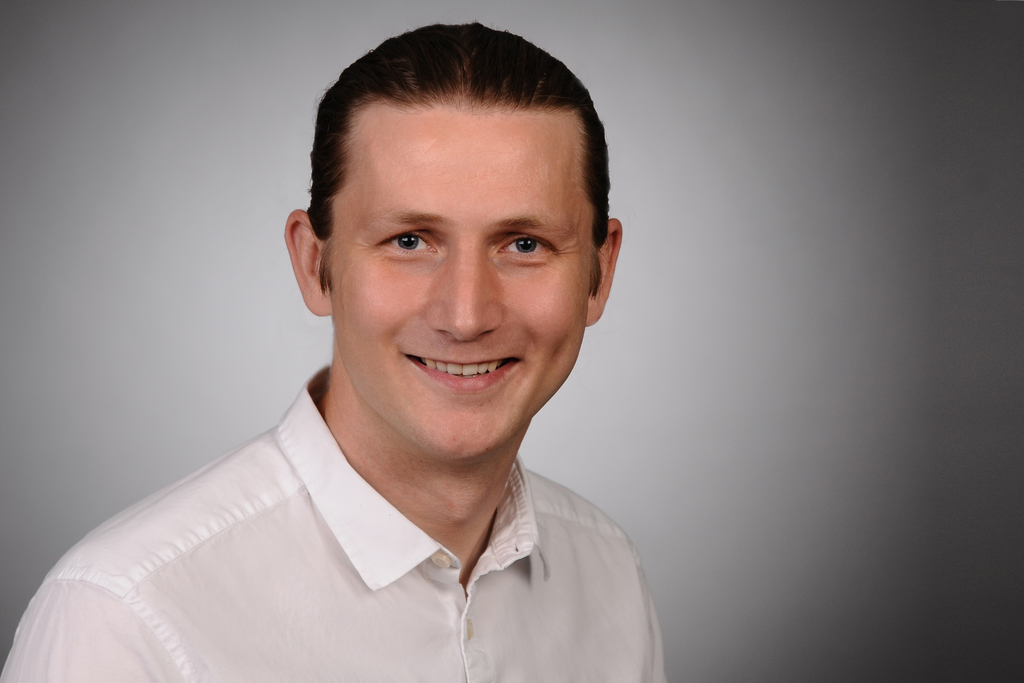
\includegraphics[width=0.25\textwidth,height=\textheight]{fig/huber2.jpeg}
\caption[\label{fig:itsme} Prof.~Dr.~Stephan Huber]{\label{fig:itsme} Prof.~Dr.~Stephan Huber\footnotemark{}}
\end{figure}
\footnotetext{Picture is taken from \url{https://sites.google.com/view/stephanhuber}}

Prof.~Dr.~Stephan Huber is Professor of International Economics and Data Science at \emph{HS Fresenius} and holds a Diploma in Economics from the \emph{University of Regensburg} and a Doctoral Degree (summa cum laude) from the University of Trier. He completed postgraduate studies at the \emph{Interdisciplinary Graduate Center of Excellence at the Institute for Labor Law and Industrial Relations in the European Union (IAAEU)} in Trier. He was a research assistant to Prof.~Dr.~Dr.~h.c. Joachim Möller at the \emph{University of Regensburg}, post-doc at the \emph{Leibniz Institute for East and Southeast European Studies (IOS)} in Regensburg and freelancer at \emph{Charles University} in Prague.

He has worked as a lecturer at various institutions including the \emph{TU Munich}, the \emph{University of Regensburg}, \emph{Saarland University}, and the \emph{Universities of Applied Sciences in Frankfurt and Augsburg}. He has also taught abroad for the \emph{University of Cordoba} in Spain and the \emph{University of Perugia}. Professor Huber has published his work in international journals such as the \emph{Canadian Journal of Economics} and the \emph{Stata Journal}. More on his work can be found on his private homepage \href{https://www.t1p.de/stephanhuber}{www.t1p.de/stephanhuber}.

\textbf{Contact}

\begin{verbatim}
   Hochschule Fresenius für Wirtschaft & Medien GmbH
   Im MediaPark 4c
   50670 Cologne
   
   Office: 4b OG-1 Bü01 (Office hour: Thursday 1-2 p.m.)
   Telefon: +49 221 973199-523
   Mail: stephan.huber@hs-fresenius.de
   Private homepage: www.t1p.de/stephanhuber
\end{verbatim}

\hypertarget{about-this-course}{%
\section*{About this course}\label{about-this-course}}

\textbf{Workload:}
125 h = 42 h (in-class) + 21 h (guided private study hours) - 62 h (private self-study).

\textbf{Assessment}
Students complete this module with a written exam of 90 minutes. A passing grade in this module is achieved when the overall grade is greater than or equal to 4.0.

\textbf{Learning outcomes:}
After successful completion of the module, students are able to:

\begin{itemize}
\tightlist
\item
  describe how tools of standard price theory, location theory, production theory, and the theory of investment decision can be employed to formulate a decision problem,
\item
  evaluate alternative courses of action and choose among alternatives,
\item
  apply economic concepts and techniques in evaluating strategic business decisions taken by firms,
\item
  apply the knowledge of the mechanics of supply and demand to explain the functioning of markets.
\end{itemize}

\textbf{How to prepare for the exam:}
I am convinced that reading the lecture notes, preparing for class, taking actively part in class, and trying to solve the exercises without going straight to the solutions is the best method for students to

\begin{itemize}
\tightlist
\item
  maximize leisure time and minimize the time needed to prepare for the exam, respectively,
\item
  getting long-term benefits out of the course,
\item
  improve grades, and
\item
  have more fun during lecture hours.
\end{itemize}

\textbf{Literature:}
\citet{Bazerman2017Judgement}, \citet{Hoover2020Introduction}, \citet{Parkin2017Economics}, \citet{Wilkinson2022Managerial}, \citet{Bonanno2017Decision}

\textbf{Content:}

\hypertarget{price-theory}{%
\paragraph*{Price theory}\label{price-theory}}
\addcontentsline{toc}{paragraph}{Price theory}

\begin{itemize}
\tightlist
\item
  the market price of an efficient competitive market and sources of inefficiency
\item
  the impact of supply and demand on the market price
\item
  the output and price decision of a profit maximizing monopolist
\item
  regional market power and price setting
\end{itemize}

\hypertarget{production-and-cost-theory}{%
\paragraph*{Production and cost theory}\label{production-and-cost-theory}}
\addcontentsline{toc}{paragraph}{Production and cost theory}

\begin{itemize}
\tightlist
\item
  output and costs of firms in the short and long run
\item
  optimization under constraints (Lagrangian multiplier)
\item
  cost--volume--profit analysis
\end{itemize}

\hypertarget{location-theory}{%
\paragraph*{Location theory}\label{location-theory}}
\addcontentsline{toc}{paragraph}{Location theory}

\begin{itemize}
\tightlist
\item
  Hotelling's location model
\item
  Thünen's model of agricultural land use
\item
  location fundamentals and agglomeration forces (sharing, matching, learning)
\end{itemize}

\hypertarget{strategic-behaviour-of-firms}{%
\paragraph*{Strategic behaviour of firms}\label{strategic-behaviour-of-firms}}
\addcontentsline{toc}{paragraph}{Strategic behaviour of firms}

\begin{itemize}
\tightlist
\item
  nature, scope, and elements of game theory
\item
  static games (Nash, Cournot, and Bertrand equilibrium)
\item
  limitations
\end{itemize}

\hypertarget{investment-decisions}{%
\paragraph*{Investment decisions}\label{investment-decisions}}
\addcontentsline{toc}{paragraph}{Investment decisions}

\begin{itemize}
\tightlist
\item
  net present value
\item
  internal rate of return
\item
  decision-making under risk
\item
  decision-making under uncertainty
\item
  common pitfalls in investment decisions
\end{itemize}

\hypertarget{about-how-to-learn-and-prepare-for-the-exam}{%
\subsection*{About how to learn (and prepare for the exam)}\label{about-how-to-learn-and-prepare-for-the-exam}}

\begin{figure}
\centering
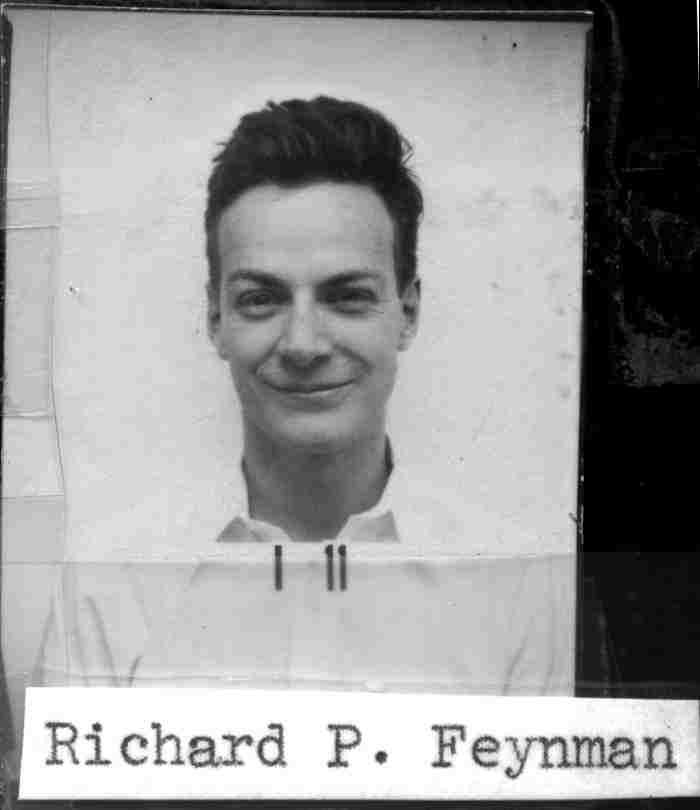
\includegraphics[width=0.25\textwidth,height=\textheight]{fig/Richard-Feynman.jpg}
\caption[\label{fig:feynman} Richard P. Feynman's badge photo from Los Alamos National Laboratory]{\label{fig:feynman} Richard P. Feynman's badge photo from Los Alamos National Laboratory\footnotemark{}}
\end{figure}
\footnotetext{Picture is taken from \url{https://repository.aip.org/islandora/object/nbla\%3A299600}}

Richard P. Feynman:

\begin{quote}
``I don't know what's the matter with people: they don't learn by understanding; they learn by some other way ­ by rote, or something. Their knowledge is so fragile!''
\end{quote}

Stephan Huber:

\begin{quote}
``I agree with Feynman: The key to learning is understanding. However, I believe that there is no understanding without practice, that is, solving problems and exercises by yourself with a pencil and a blank sheet of paper without knowing the solution in advance.''
\end{quote}

\begin{itemize}
\tightlist
\item
  Study the lecture notes, i.e., try to understand the exercises and solve them yourself.
\item
  Study the exercises, i.e., try to understand the logical rules and solve the problems yourself.
\item
  Test yourself with past exams that you will find on ILIAS. The structure of the exam is more or less the same every semester.
\item
  If you have the opportunity to form a group of students to study and prepare for the exam, make use of it. It is great to help each other, and it is very motivating to see that everyone has problems sometimes.
\item
  If you have difficulties with some exercises and the solutions shown do not solve your problem, ask a classmate or contact me. I will do my best to help.
\end{itemize}

\hypertarget{what-is-managerial-economics}{%
\chapter{What is managerial economics?}\label{what-is-managerial-economics}}

\begin{center}\rule{0.5\linewidth}{0.5pt}\end{center}

After successful completion of the module, students are able to:

\begin{itemize}
\tightlist
\item
  Explain what managerial economics is all about.
\item
  Discuss the use of managerial econmics for their private and professional lifes.
\item
  Explain how managerial economics relates to other disciplines of social sciences.
\end{itemize}

\begin{center}\rule{0.5\linewidth}{0.5pt}\end{center}

Well, that's a question that can't be answered definitively. It is whatever you would like it to be. Each instructor may find a slightly different way to define what it is. However, there are some conventions for what many people mean by it. To find out what most people mean by managerial economics, public and general sources like Wikipedia are a good source.\footnote{Usually, it is not a good idea to cite Wikipedia in an academic paper, because everything written down in Wikipedia has to come from some other source. So Wikipedia is usually only a secondary source. However, general definitions of an important topic are sometimes worth citing, as they can be seen as a definition that is at least accepted by a more or less large group of administrators who can make changes to Wikipedia}.

More recent, many people start using ChatGPT for good reasons. \citet{Korinek2023Language} discusses the use of it for academic research. Lets see what ChatGPT and Wikipedia say about managerial economics.

\hypertarget{what-is-managerial-economics-for-chatgpt}{%
\section{What is managerial economics for ChatGPT?}\label{what-is-managerial-economics-for-chatgpt}}

\textbf{Define managerial economics.}

ChatGPT: Managerial economics is the application of economic theories, concepts, and analytical tools to solve managerial problems in business organizations. It involves the study of how economic principles can be applied to make better decisions regarding the allocation of resources, production and consumption of goods and services, pricing strategies, market analysis, and other strategic issues facing firms. The main goal of managerial economics is to provide managers with a framework to analyze business problems and make informed decisions that will maximize the firm's profits and shareholder value. It is an interdisciplinary field that draws from economics, finance, accounting, statistics, and other related fields to help managers understand the economic environment in which they operate and make effective decisions.

\textbf{What distinguishes managerial economics from Microeconomics and Macroeconomics?}

ChatGPT: Managerial economics is closely related to both microeconomics and macroeconomics, but it differs from these two branches of economics in several ways:

\begin{enumerate}
\def\labelenumi{\arabic{enumi}.}
\item
  Scope: Microeconomics focuses on the behavior of individual economic agents, such as households and firms, while macroeconomics focuses on the behavior of the economy as a whole, including variables such as aggregate output, employment, and inflation. Managerial economics, on the other hand, focuses on the decision-making behavior of individual firms, and how they interact with the market and other firms.
\item
  Purpose: The purpose of microeconomics is to study the allocation of resources among different uses and the interactions of individual agents in the market, while macroeconomics is concerned with the overall performance of the economy. Managerial economics, on the other hand, is concerned with applying economic principles to solve managerial problems in business organizations, such as pricing strategies, cost analysis, and production decisions.
\item
  Analysis: Microeconomics uses mathematical and graphical models to analyze the behavior of individual agents in the market, while macroeconomics uses aggregate economic data to study the overall performance of the economy. Managerial economics, however, uses both microeconomic and macroeconomic tools and techniques to analyze and solve specific managerial problems.
\item
  Perspective: Microeconomics takes the perspective of an individual economic agent, while macroeconomics takes the perspective of the entire economy. Managerial economics, on the other hand, takes the perspective of the manager and the firm, and how they can use economic principles to make better decisions.
\end{enumerate}

\emph{In summary, while managerial economics draws from both microeconomics and macroeconomics, it focuses on the specific issues facing firms and their decision-making behavior, making it distinct from these other two branches of economics.}

\hypertarget{what-is-managerial-economics-for-wikipedia}{%
\section{What is managerial economics for Wikipedia?}\label{what-is-managerial-economics-for-wikipedia}}

Read \url{https://en.wikipedia.org/wiki/Managerial_economics}

\hypertarget{simple-definition-of-managerial-economics}{%
\section{Simple definition of managerial economics}\label{simple-definition-of-managerial-economics}}

To me managerial economics is economics for managers. That means, any sort of method, information, and knowledge from economic research that can help managers somehow in making good decisions and achieve their goals can be considered to be part of managerial economics. So, now we can discuss what \emph{economics} is all about and what therein can be helpful to managers.

\hypertarget{what-is-economics}{%
\section{What is economics?}\label{what-is-economics}}

All economic questions arise because we want more than we can get. Our inability to satisfy all our wants is called scarcity and because of scarcity, we must make choices that depend on the incentives we face. An incentive is a reward that encourages or a penalty that discourages an action.

Economics is a social science, and as in all social sciences, many of the terms used in it are poorly defined. The following quotes can demonstrate that:

\begin{quote}
John Maynard Keynes (1883-1946): ``The theory of economics does not furnish a body of settled conclusions immediately applicable to policy. It is a method rather than a doctrine, an apparatus of the mind, a technique of thinking, which helps it possessors to draw correct conclusions.'' \citet{Keynes1921Introduction}
\end{quote}

\begin{quote}
Alfred Marshall (1842-1924): ``Economics is a study of mankind in the ordinary business of life; it examines that part of individual and social action which is most closely connected with the attainment and with the use of the material requisites of wellbeing.'' \citet[p.~1]{Marshall2009Principles}
\end{quote}

\begin{quote}
Gary S. Becker (1930-2014): ``Economics is all about how people make choices. Sociology is about why there isn't any choice to be made.'' \citet[p.~233]{Becker1960Economic}
\end{quote}

\begin{quote}
\citet[p.~4]{Colander2006Economics}: ``Economics is the study of how human beings coordinate their wants and desires, given the decision-making mechanisms, social customs, and political realities of the society.''
\end{quote}

\begin{quote}
\citet[p.~2]{Parkin2012Economics}: ``Economics is the social science that studies the choices that individuals, businesses, governments, and entire societies make as they cope with scarcity and the incentives that influence and reconcile those choices.''
\end{quote}

\begin{quote}
\citet[p.~5.]{Gwartney2006Microeconomics}: ``{[}E{]}conomics is the study of human behavior, with a particular focus on human decision making.''
\end{quote}

\begin{quote}
\citet[p.~222]{Backhouse2009Retrospectives}: ``{[}E{]}conomics is apparently the study of the economy, the study of the coordination process, the study of the effects of scarcity, the science of choice, and the study of human behavior.''
\end{quote}

\begin{quote}
\citet[ch.~1]{Greenlaw2018Principles}: Economics seeks to solve the problem of scarcity, which is when human wants for goods and services exceed the available supply. A modern economy displays a division of labor, in which people earn income by specializing in what they produce and then use that income to purchase the products they need or want. The division of labor allows individuals and firms to specialize and to produce more for several reasons: a) It allows the agents to focus on areas of advantage due to natural factors and skill levels; b) It encourages the agents to learn and invent; c) It allows agents to take advantage of economies of scale. Division and specialization of labor only work when individuals can purchase what they do not produce in markets. Learning about economics helps you understand the major problems facing the world today, prepares you to be a good citizen, and helps you become a well-rounded thinker.
\end{quote}

\begin{quote}
\citet[p.~222]{Backhouse2009Retrospectives}: ``Perhaps the definition of economics is best viewed as a tool for the first day of principles classes but otherwise of little concern to practicing economists.''
\end{quote}

\begin{quote}
Jacob Viner (1892-1970): ``Economics is what economists do.'' \citet[p.~222]{Backhouse2009Retrospectives}
\end{quote}

\begin{quote}
\citet[p.~2]{Parkin2012Economics}: ``Microeconomics is the study of the choices that individuals and businesses make, the way these choices interact in markets, and the influence of governments. {[}\ldots{]} Macroeconomics is the study of the performance of the national economy and the global economy.''
\end{quote}

Although many textbook definitions are quite similar in many ways, the
lack of agreement on a clear-cut definition of economics does not really matter and does not necessarily pose a problem as

\begin{quote}
``{[}E{]}conomists are generally guided by pragmatic considerations of what works or by methodological views emanating from various sources, not by formal definitions.'' \citet[p.~231]{Backhouse2009Retrospectives}
\end{quote}

\textbf{The important questions of economics:}
How do choices end up determining what, where, how, and for whom goods and services get produced? And: When do choices made in the pursuit of self-interest also promote the social interest?

\hypertarget{decision-making-basics}{%
\chapter{Decision making basics}\label{decision-making-basics}}

\begin{center}\rule{0.5\linewidth}{0.5pt}\end{center}

After successful completion of the module, students are able to:

\begin{itemize}
\tightlist
\item
  Make decisions with a great awareness of the nature of the decision and the purpose of making a decision.
\item
  Explain the trade-offs that should be taken into account when making a decision.
\item
  Explain different characteristics of decisions.
\item
  Take advantage of various decision making strategies.
\item
  Explain the rational model of decision making and the concept of the homo economicus.
\item
  Explain the bounded rationality of humans and its implications on their ability to make decisions.
\item
  Apply heuristics to make good decisions.
\end{itemize}

\begin{center}\rule{0.5\linewidth}{0.5pt}\end{center}

\hypertarget{exercises-to-reflect-on-how-we-make-decisions}{%
\section{Exercises to reflect on how we make decisions}\label{exercises-to-reflect-on-how-we-make-decisions}}

\begin{exercise}
\protect\hypertarget{exr:brain-color}{}\label{exr:brain-color}Brain

\begin{figure}
\centering
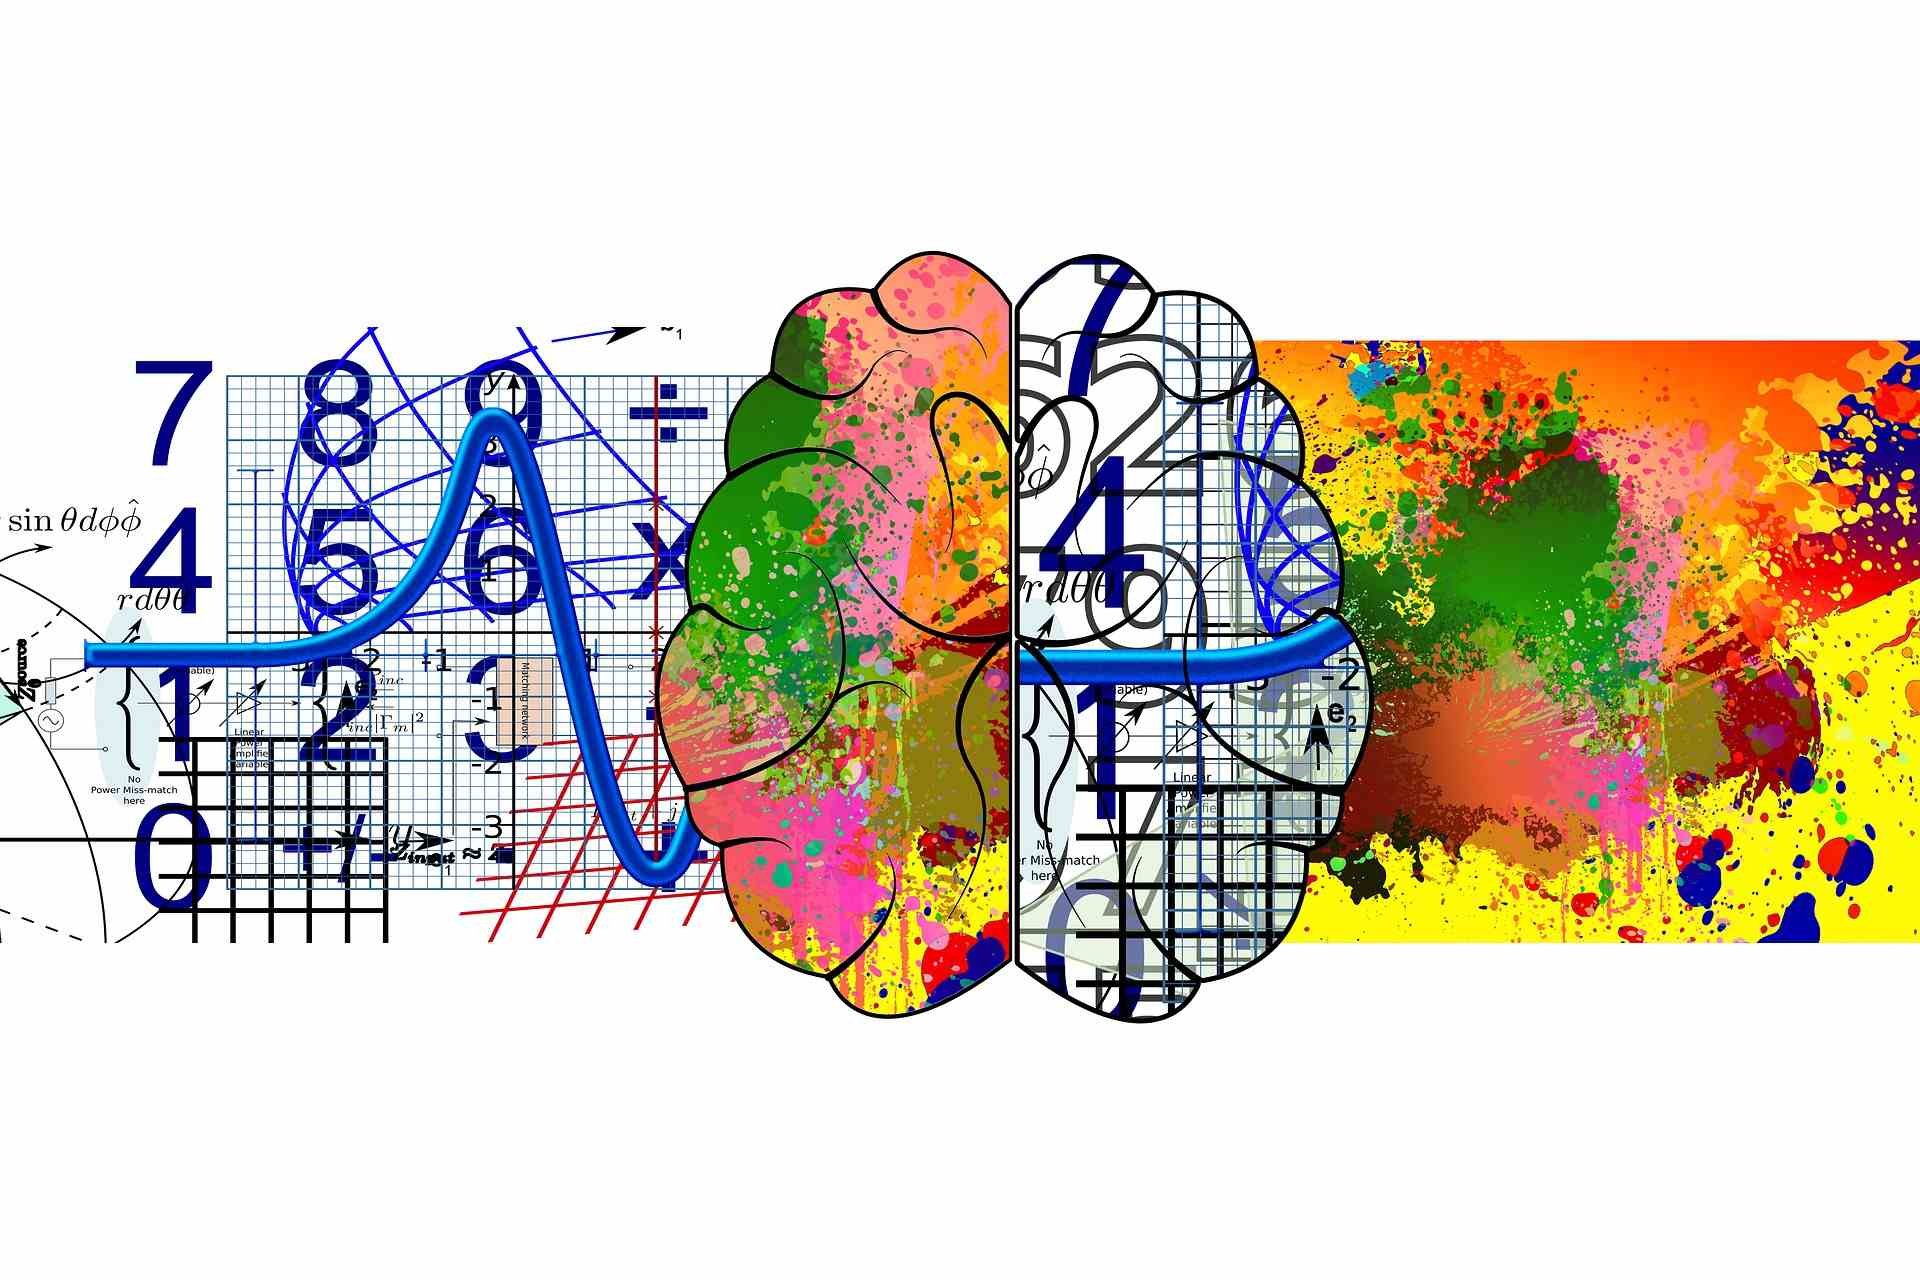
\includegraphics[width=1\textwidth,height=\textheight]{fig/brain-color.jpg}
\caption[\label{fig:brain-color} From data to decision]{\label{fig:brain-color} From data to decision\footnotemark{}}
\end{figure}
\footnotetext{Source: \url{https://pixabay.com/images/id-6671455/}}

Discuss figure \ref{fig:brain-color}. What is the message of the picture?
\end{exercise}

\begin{exercise}
\protect\hypertarget{exr:puzzle}{}\label{exr:puzzle}Solve the puzzles

\begin{enumerate}
\def\labelenumi{\alph{enumi})}
\tightlist
\item
  \textbf{The nine dots problem}
  Connect the dots shown in fugure \ref{fig:9dots} with no more than 4 straight lines without lifting your hand from the paper.
\end{enumerate}

\begin{figure}
\centering

\includegraphics[width=0.15\textwidth,height=\textheight]{fig/9dots.png}
\caption{\label{fig:9dots} The nine dots problem}
\end{figure}

\begin{enumerate}
\def\labelenumi{\alph{enumi})}
\setcounter{enumi}{1}
\tightlist
\item
  \textbf{The tasty cake puzzle} In figure \ref{fig:cake} you see a tasty cake with the nine dots representing strawberries. Cut this cake up with exactly four straight cuts so that each portion of the cake contains just one strawberry on the top.
\end{enumerate}

\begin{figure}
\centering
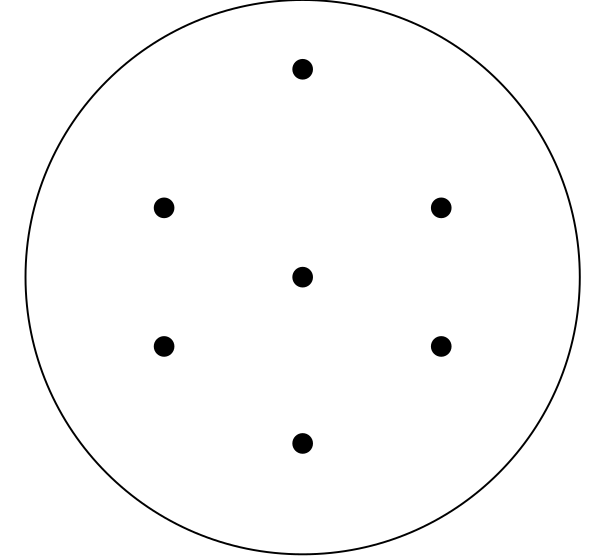
\includegraphics[width=0.25\textwidth,height=\textheight]{fig/cake.png}
\caption{\label{fig:cake} The tasty cake puzzle}
\end{figure}

Reflect on how you tried to solve the puzzles. Did you have a problem solving strategy? How did you come to the right decision? Think of restrictions you imposed on yourself which was not inherent to the problem.
\end{exercise}

\begin{exercise}
\protect\hypertarget{exr:santa}{}\label{exr:santa}What is the house of Santa Claus?

The house of Santa Claus is an old German drawing game. It goes like this: You have to draw a house in one line where you (a) must start at bottom left (point 1), (b) you are not allowed to lift your pencil while drawing and (c) it is forbidden to repeat a line. During drawing you say: ``Das ist das Haus des Nikolaus'\,'. What do you think is the success-rate of kids who play this game for the first time?

\begin{figure}
\centering
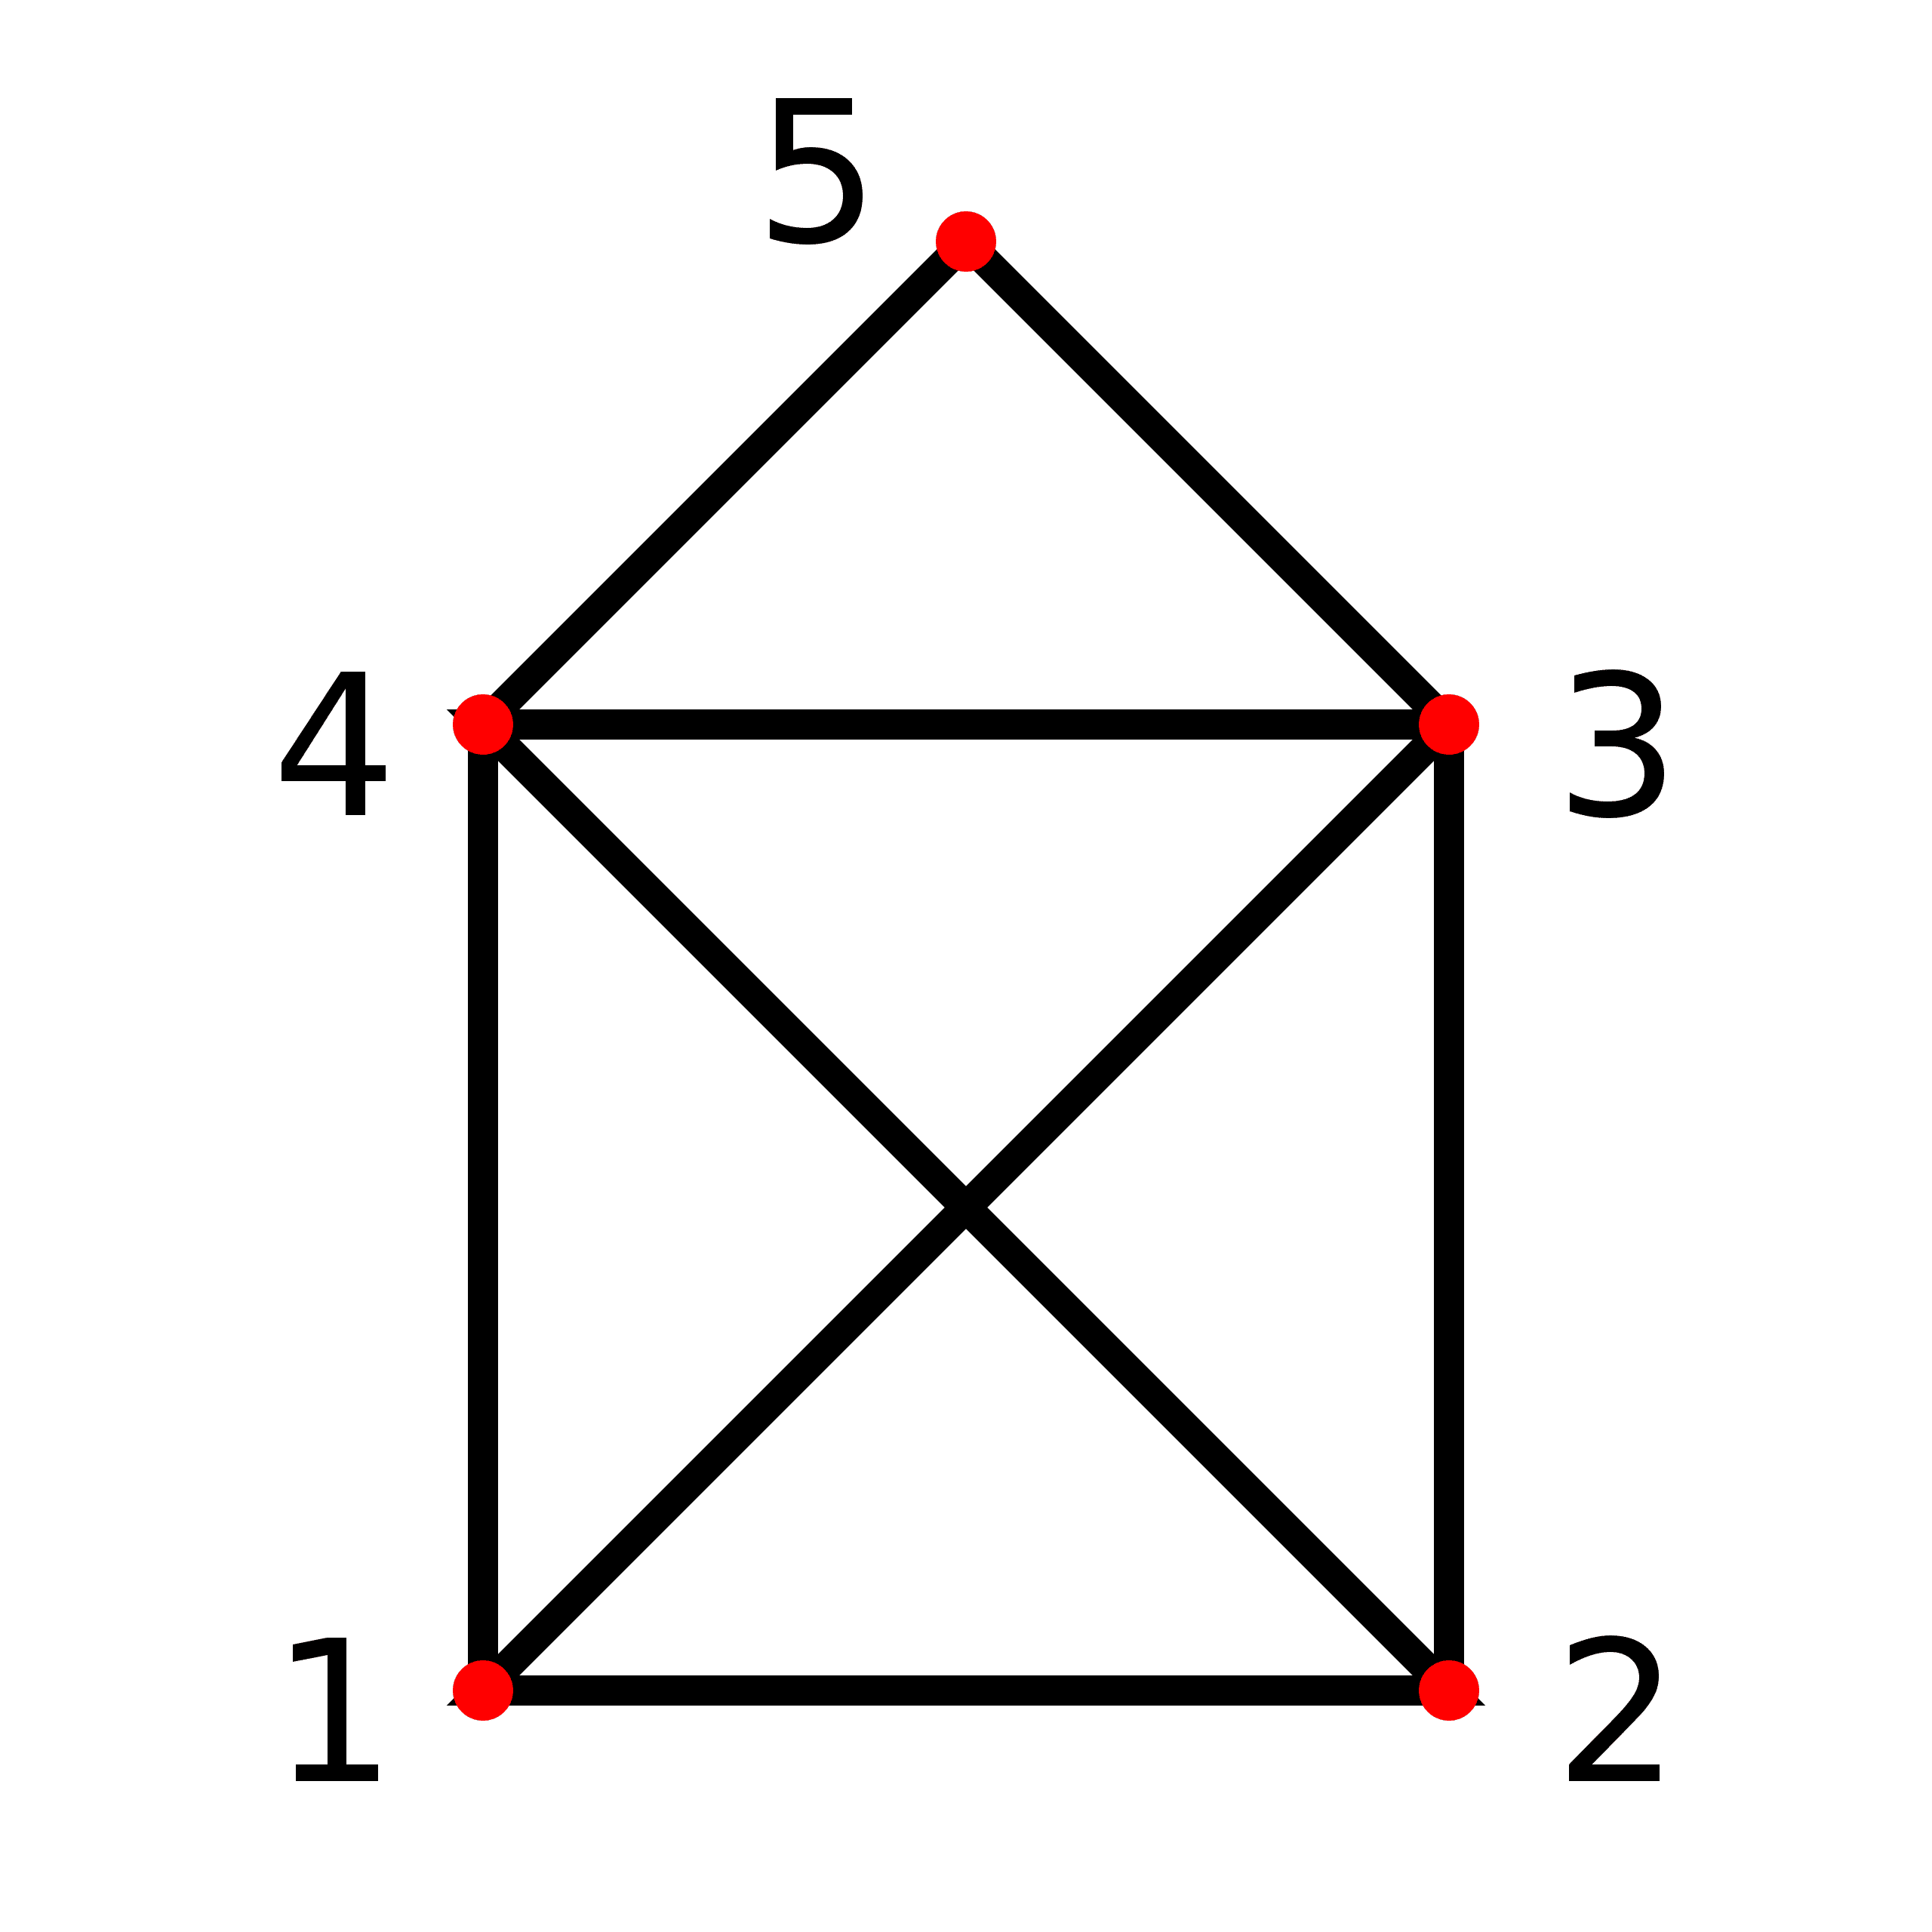
\includegraphics[width=0.25\textwidth,height=\textheight]{fig/nikolaus.png}
\caption{\label{fig:nikolaus} The house of Santa Claus}
\end{figure}

\begin{figure}
\centering

\includegraphics[width=0.2\textwidth,height=\textheight]{fig/pingo666528.png}
\caption{\label{fig:pingo} PINGO}
\end{figure}

Answer the question here:
\url{https://pingo.coactum.de/}
Code: 666528

Please find solution to the exercise \protect\hyperlink{sol:santa}{in the appendix}
\end{exercise}

\hypertarget{what-defines-a-decision}{%
\section{What defines a decision?}\label{what-defines-a-decision}}

The statement of \citet{Eilon1969What} still holds true:

\begin{quote}
``An examination of the literature reveals the somewhat perplexing fact that most books on management and decision theory do not contain a specific definition of what is meant by a decision. One can find detailed descriptions of decision trees, discussions of game theory and analyses of various statistical treatments of payoffs matrices under conditions of uncertainty, but the definition of the decision activity itself is often taken for granted and is associated with making a choice between alternative courses of action.''
\end{quote}

The word \emph{decision} stems from the latin verb \emph{decidere} which can have different meanings\footnote{See \url{http://www.latin-dictionary.net/search/latin/decidere}} including make explicit, put an end to, bring to conclusion, settle/decide/agree (on), die, end up, fail, fall in ruin, fall/drop/hang/flow down/off/over, sink/drop, cut/notch/carve to delineate, detach, cut off/out/down, fell, flog thoroughly.

Wikipedia defines \textbf{decision making} as follows:

\begin{quote}
``In psychology, decision-making {[}\ldots{]} is regarded as the cognitive process resulting in the selection of a belief or a course of action among several alternative possibilities. Decision-making is the process of identifying and choosing alternatives based on the values, preferences and beliefs of the decision-maker. Every decision-making process produces a final choice, which may or may not prompt action. {[}\ldots{]} Decision-making can be regarded as a problem-solving activity yielding a solution deemed to be optimal, or at least satisfactory. It is therefore a process which can be more or less rational or irrational\ldots{}''
\end{quote}

Businessdictionary.com defines a \textbf{decision} as

\begin{quote}
``A choice made between alternative courses of action in a situation of uncertainty.''
\end{quote}

Let's agree on the following working definition that is symbolized in figure \ref{fig:decisionm}:

\begin{quote}
A decision is the point at which a choice is made between alternative---and usually competing---options. As such, it may be seen as a stepping-off point---the moment at which a commitment is made to one course of action to the exclusion of others. (Fitzgerald, 2002, p.~8)
\end{quote}

\begin{figure}
\centering
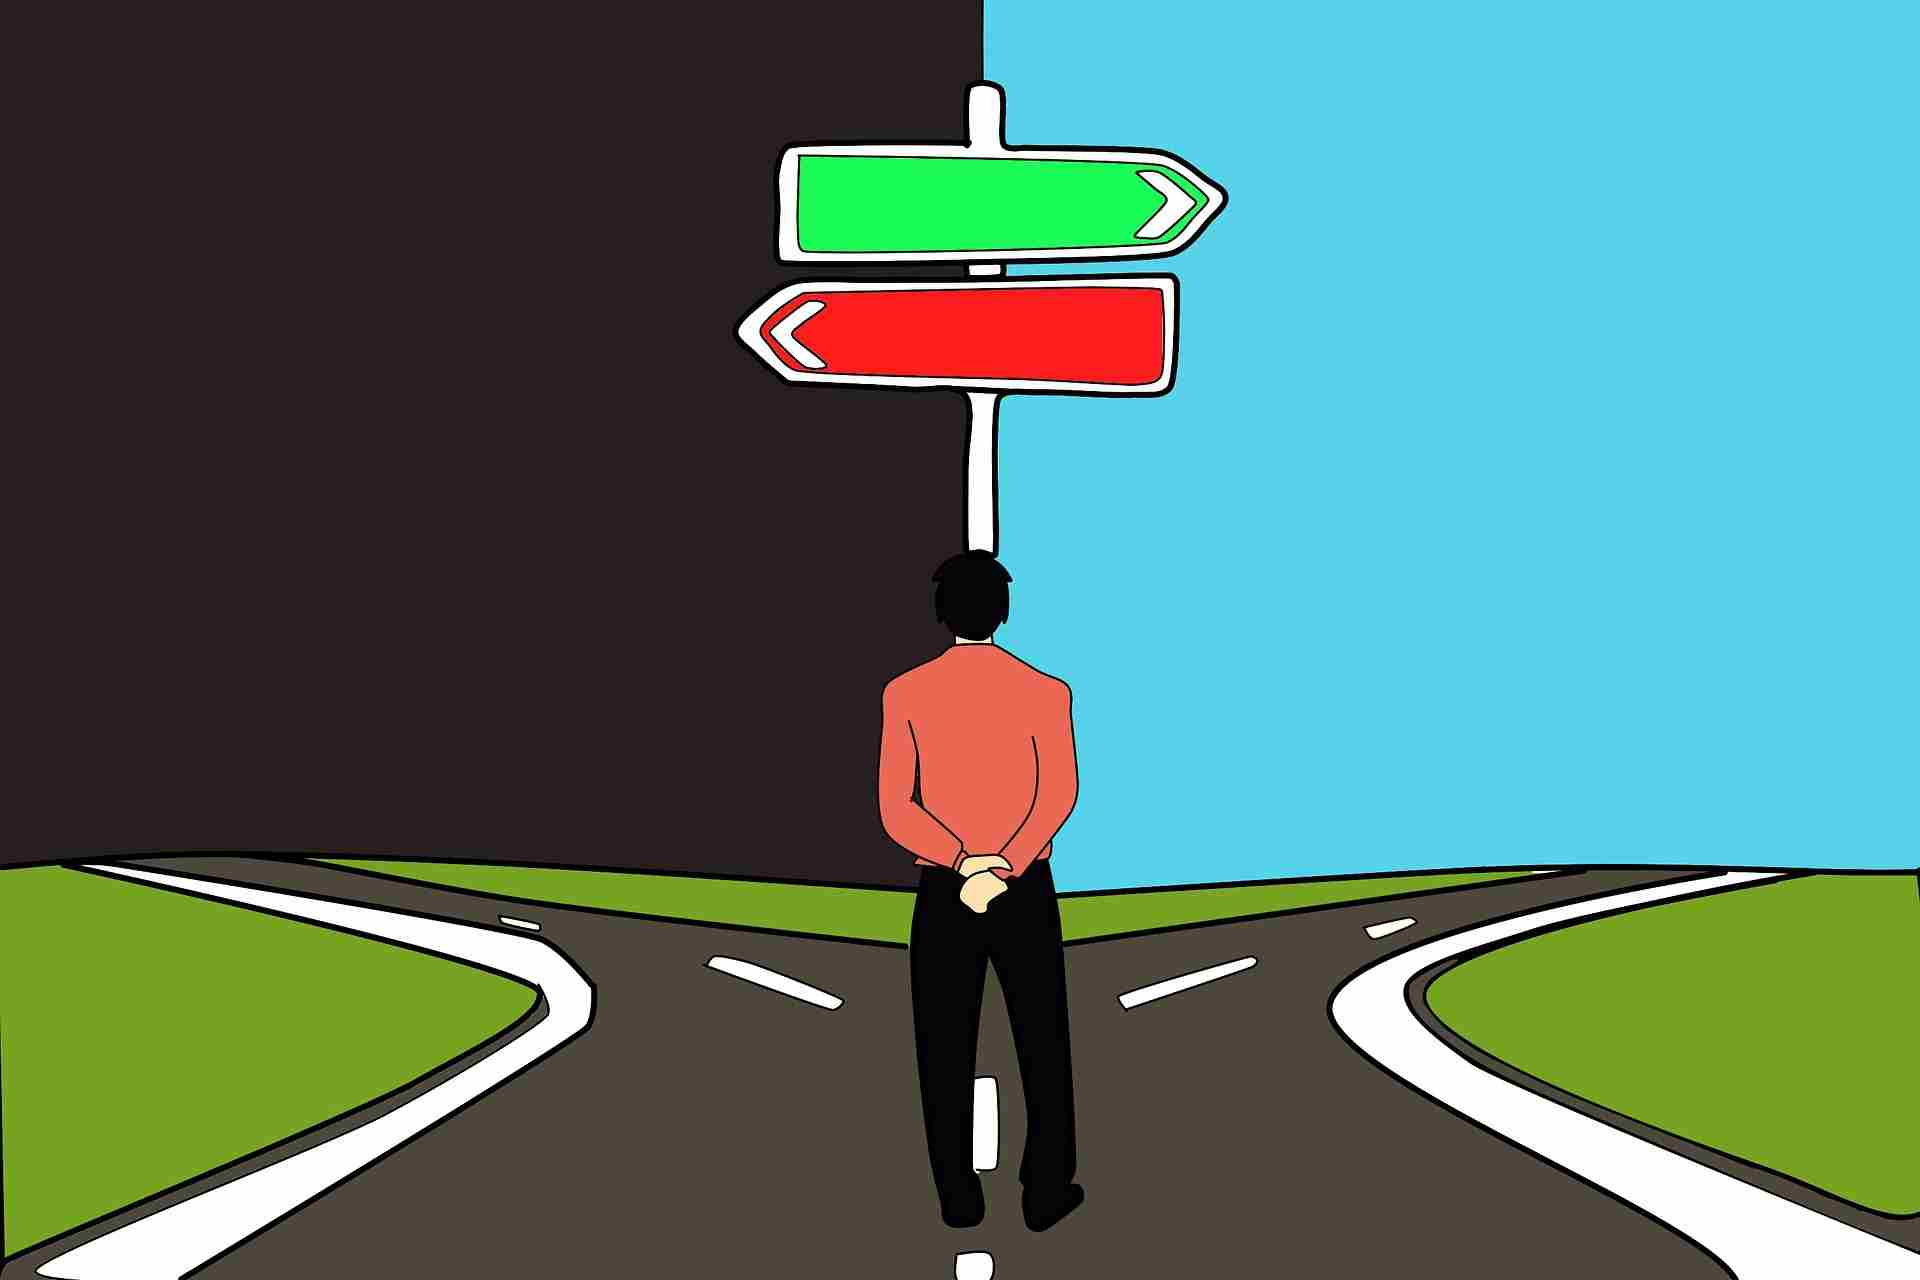
\includegraphics[width=0.5\textwidth,height=\textheight]{fig/decision-making.jpg}
\caption[\label{fig:decisionm} Decision-making]{\label{fig:decisionm} Decision-making\footnotemark{}}
\end{figure}
\footnotetext{Picture is taken from \url{https://pixabay.com/de/illustrations/entscheidung-auswahl-pfad-stra\%C3\%9Fe-1697537/}}

\hypertarget{types-of-decisions}{%
\section{Types of decisions}\label{types-of-decisions}}

Decision making is a process of investing time and effort to make a decision that will lead to (good) results. In the following, we discuss some types of decisions that can help to design an appropriate decision making process.

According to \citet[p.~9f]{Fitzgerald2002Decision} decisions can be roughly divided into two generic types:

\begin{itemize}
\tightlist
\item
  \textbf{routine decisions}: Decisions that must be made at regular intervals.
\item
  \textbf{non-routine}: Unique, random, non-recurring decision situations.
\end{itemize}

Another common method of dividing decisions into two categories is as follows:

\begin{itemize}
\tightlist
\item
  \textbf{Operative decisions}: This type of decision usually involves day-to-day business operations. There is a lot of overlap with the routine category here. Examples of this type of decision include setting production levels, deciding whether to hire or deciding whether to close a particular plant. When it comes to decisions in our daily lives, an example would be where, what, when, and what we eat for lunch.
\item
  \textbf{Strategic decisions}: This type of decision is usually about company policy and direction over a long period of time. Examples of strategic decisions include entering a new market, acquiring a competitor, or withdrawing from an industry. Renting an apartment near the university or commuting to our parents is an example of a strategic decision in our personal lives.
\end{itemize}

People often distinguish between decisions at work and private decisions. Private decisions affect fewer people on average, but usually the people involved are closer to you personally. However, both types of decisions involve the same things such as people (human resources), money (budgeting), buying and selling (marketing), how we do something (operations) or how we want to do it in the future (strategy and planning).

Some decisions are more important than others because the potential impact of a decision varies, i.e., the \textbf{scope of a decision}. For example, decisions can affect one person or millions, one pound/dollar or millions, one product/service or an entire market, one day or ten years, etc.

However, it is not entirely clear how to validate the scope. It depends heavily on the perspective of the decision-maker. For a small company, for example, an investment of 10,000 euros may be a big decision, while for a multinational cooperation it is a drop in the bucket. So the scope for decisions is relative, not absolute. It depends entirely on the context in which the decision is made and on the characteristics of the person(s) making it.

\hypertarget{three-conditions-of-decision-making}{%
\section{Three conditions of decision making}\label{three-conditions-of-decision-making}}

\begin{figure}
\centering
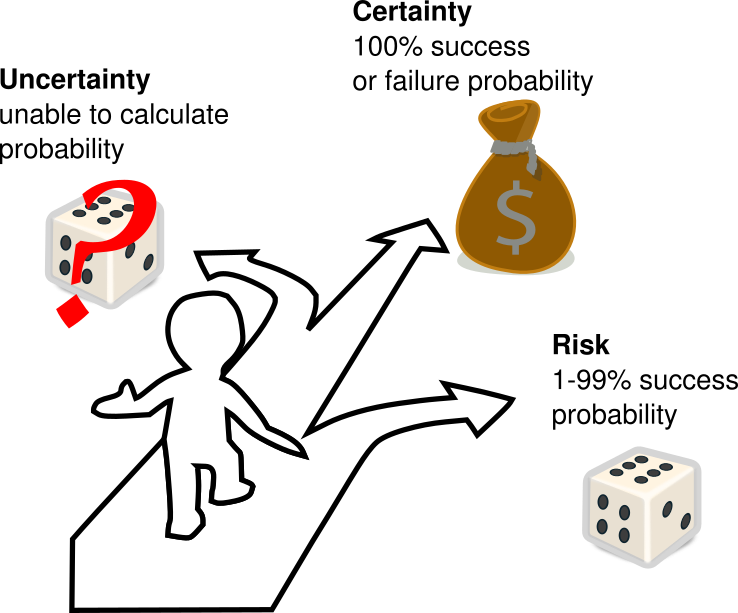
\includegraphics[width=0.5\textwidth,height=\textheight]{fig/risk-certainty-uncertainty.png}
\caption[\label{fig:3conditions} Conditions of decision making]{\label{fig:3conditions} Conditions of decision making\footnotemark{}}
\end{figure}
\footnotetext{Source: \citet{CEOpedia2021Rational}}

There are three general conditions (see \ref{fig:3conditions}) that determine the design of the optimal decision making process: certainty, risk and uncertainty.

\textbf{Certainty:}
A condition under which taking a decision involves reasonable degree of certainty about its result, what are the opportunities and what conditions accompany this decision.

\textbf{Risk:}
A condition under which taking a decision involves reasonable degree of certainty about its result, what are the opportunities and what conditions accompany this decision.

\textbf{Uncertainty:}
A condition in which decision maker does not know all the choices, as well as risks associated with each of them and possible consequences.

\hypertarget{decision-making-strategies}{%
\section{Decision making strategies}\label{decision-making-strategies}}

\begin{exercise}
\protect\hypertarget{exr:decisionstrategy}{}\label{exr:decisionstrategy}

Different schemes of a decision making process

\begin{enumerate}
\def\labelenumi{\alph{enumi})}
\item
  Google for \emph{``decision making strategies''} and look at the images that Google suggests you.
\item
  Read \citet{IET202312} and discuss the twelve decision making strategies. The article can be found \href{https://www.indeed.com/career-advice/career-development/decision-making-strategies?utm_campaign=earnedsocial\%3Acareerguide\%3Asharedirectshare\%3AUS\&utm_content=12\%20Decision-Making\%20Strategies\&utm_medium=social\&utm_source=directshare}{here}.
\item
  Compare these strategies to the scheme shown in figure \ref{fig:decision}.
\end{enumerate}

\begin{figure}
\centering
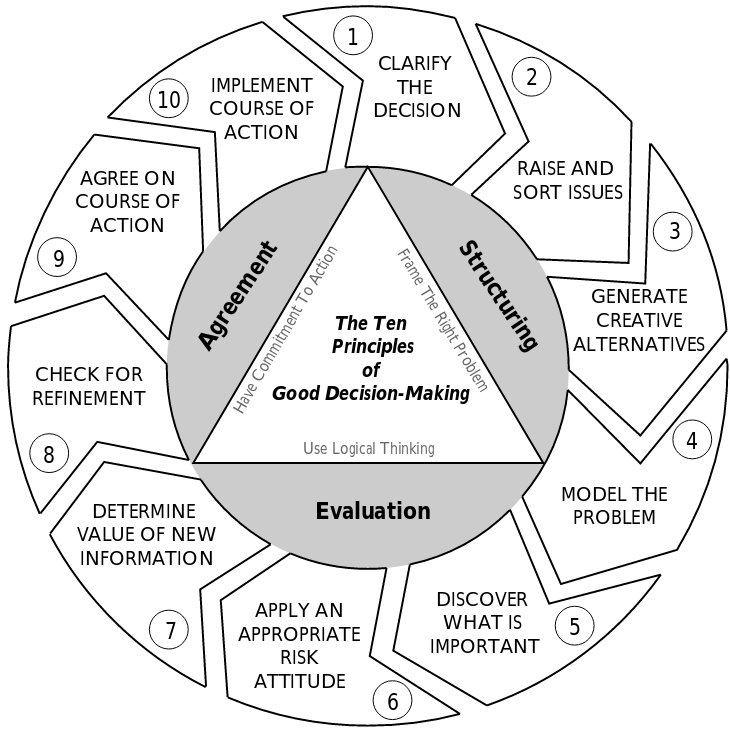
\includegraphics[width=0.5\textwidth,height=\textheight]{fig/tenprincipals_png.png}
\caption[\label{fig:decision} Decision-making]{\label{fig:decision} Decision-making\footnotemark{}}
\end{figure}
\footnotetext{Picture is taken from \url{https://pixabay.com/de/illustrations/entscheidung-auswahl-pfad-stra\%C3\%9Fe-1697537/}}

\begin{enumerate}
\def\labelenumi{\alph{enumi})}
\setcounter{enumi}{3}
\item
  Choose a problem of your choice and try to solve the problem using the two illustrations above by making a good decision.
\item
  Discuss in class whether the diagram or the strategies in \citet{IET202312} are helpful in making a wise decision or solving a problem.
\item
  Watch \url{https://youtu.be/pPIhAm_WGbQ} and answer the following questions: How is the nature of decisions discussed here? Does it contain a rational model of problem solving? Reflect on which ways to solve a problem and come to a decision, respectively, have been addressed.
\end{enumerate}

\end{exercise}

\begin{exercise}
\protect\hypertarget{exr:fisherman}{}\label{exr:fisherman}The businessman and the fisherman

A classic tale that exist in different version\^{}{[}This one stems from \href{https://thestorytellers.com/the-businessman-and-the-fisherman}{thestorytellers.com}. A famous version stems from Paulo Coelho\^{}{[}See \href{https://paulocoelhoblog.com/2015/09/04/the-fisherman-and-the-businessman/}{https://paulocoelhoblog.com} and it goes like this:

\begin{quote}
One day a fisherman was lying on a beautiful beach, with his fishing pole propped up in the sand and his solitary line cast out into the sparkling blue surf. He was enjoying the warmth of the afternoon sun and the prospect of catching a fish.

About that time, a businessman came walking down the beach, trying to relieve some of the stress of his workday. He noticed the fisherman sitting on the beach and decided to find out why this fisherman was fishing instead of working harder to make a living for himself and his family. ``You aren't going to catch many fish that way'', said the businessman to the fisherman.

``You should be working rather than lying on the beach!'' The fisherman looked up at the businessman, smiled and replied, ``And what will my reward be?'' ``Well, you can get bigger nets and catch more fish!'' was the businessman's answer. ``And then what will my reward be?'' asked the fisherman, still smiling. The businessman replied, ``You will make money and you'll be able to buy a boat, which will then result in larger catches of fish!'' ``And then what will my reward be?'''' asked the fisherman again.

The businessman was beginning to get a little irritated with the fisherman's questions. ``You can buy a bigger boat, and hire some people to work for you!'' he said. ``And then what will my reward be?'' repeated the fisherman. The businessman was getting angry. ``Don't you understand? You can build up a fleet of fishing boats, sail all over the world, and let all your employees catch fish for you!''

Once again the fisherman asked, ``And then what will my reward be?'' The businessman was red with rage and shouted at the fisherman, ``Don't you understand that you can become so rich that you will never have to work for your living again! You can spend all the rest of your days sitting on this beach, looking at the sunset. You won't have a care in the world!''

The fisherman, still smiling, looked up and said, ``And what do you think I'm doing right now?''
\end{quote}

Define the cost and benefits of both persons. Who do you think has a better life overall.
Who is acting rationally here? In other words, who is maximizing utility here? The fishermen or the businessmen? Both? None?
\end{exercise}

\hypertarget{the-rational-model}{%
\section{The rational model}\label{the-rational-model}}

Economists view the choices that people make as \emph{rational}. A rational choice is one that compares costs and benefits and achieves the greatest benefit over cost for the person making the choice. Whatever the benefits and the costs maybe, a decision maker have to consider all and make a decision. Of course, in reality it is often difficult if not impossinle to sum up benefits and costs as the nature of both may be totally different. To get rid of these problems economists use a theoretical concept that measures both in \emph{utility}. That is a general and abstract measure to model worth or value. Its usage has evolved significantly over time. The term was introduced initially as a measure of pleasure or happiness within the theory of utilitarianism. It represents the satisfaction or pleasure that people receive for consuming a bundle of goods and services, for example.

According to \citet{CEOpedia2021Rational} rational decision making is a style of decision making based on objective data and a formal process of analysis. It excludes acting based on subjective feelings and intuitive approach. The model assumes that deducting decisions with full information and all alternatives allows for the creation of cognitive skills that allow the evaluation of all possible options and then the selection of the best one.

It essentially consists of a logical sequence of steps. Here is an example taken from \citet[p.~13]{Fitzgerald2002Decision}:

\begin{enumerate}
\def\labelenumi{\arabic{enumi}.}
\item
  \textbf{Clearly identify the problem}. A \emph{problem} can be defined as a perceived gap between the current reality and the desired reality.
\item
  \textbf{Generate potential solutions}. For routine decisions, various alternatives can be identified relatively easily using predetermined decision rules, but non-routine decisions require a creative process to find new alternatives.
\item
  Using appropriate analytical approaches, select a solution from the available alternatives, preferably the one with the largest expected value. In decision theory, this is called \textbf{maximizing the expected utility of the outcomes}.
\item
  \textbf{Implement the solution}. Managers often undermine implementation by not ensuring that those responsible for implementation understand and accept what they need to do, and that they have the motivation and resources needed for successful implementation.
\item
  \textbf{Evaluate the effectiveness of the implemented decision}
\end{enumerate}

While these rational models may be helpful, they can also be criticized in a number of ways. In particular, it is a belief that managers actually optimize their decision behavior based on rationality because they consciously select and implement the best alternatives. This is a misconception because any rational optimization is based on a number of dubious assumptions. For example, (Fitzgerald, 2002, p.~13):

\begin{itemize}
\tightlist
\item
  it is hardly possible to know in advance all possible alternative solutions and to know in advance the specific outcomes that will result from each of them;
\item
  there is actually an optimal solution, and this solution is among the alternatives identified;
\item
  it is possible to accurately and numerically weight the various alternatives, the probabilities of their outcomes, and the relative desirability of these alternatives and outcomes;
\item
  the decision makers always act rationally and therefore the decision making is free of emotion, bias, and politics; and
\item
  business decisions are driven entirely by the desire to maximize profits.
\end{itemize}

The \textbf{rational model can be considered normative} because it prescribes a strict logical sequence of steps to be followed in any decision-making situation. The rational models are based on the assumption that human behavior is logical and therefore predictable under certain circumstances. This is not necessarily what actually happens in the real world. Consider, for example, the findings in the field of behavioral economics, which clearly show that homo economicus is a (useful) concept that is weak in several aspects.

\hypertarget{bounded-rationality}{%
\section{Bounded rationality}\label{bounded-rationality}}

\begin{figure}
\centering
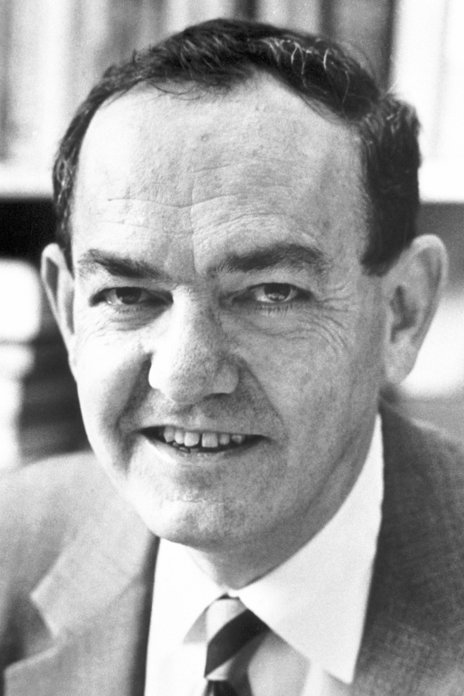
\includegraphics[width=0.2\textwidth,height=\textheight]{fig/herbert-simon.jpg}
\caption[\label{fig:simon} Herbert A. Simon]{\label{fig:simon} Herbert A. Simon\footnotemark{}}
\end{figure}
\footnotetext{Picture is taken from \href{https://www.nobelprize.org/images/simon-13300-portrait-mini-2x.jpg}{Nobel Foundation archive}}

Herbert A. Simon (1916-2001) shown in figure \ref{fig:simon} received the Nobel Memorial Prize in Economic Sciences in 1978 and the Turing Award\footnote{The Turing Award is an annual prize given by the Association for Computing Machinery (ACM) for contributions of lasting and major technical importance to the computer field. It is generally recognized as the highest distinction in computer science and is known as or often referred to as `Nobel Prize of Computing'.} in 1975. According to \citet{NobelPrize.org2021Herbert}, he

\begin{quote}
``combined different scientific disciplines and considered new factors in economic theories. Established economic theories held that enterprises and entrepreneurs all acted in completely rational ways, with the maximization of their own profit as their only goal. In contrast, Simon held that when making choices all people deviate from the strictly rational, and described companies as adaptable systems, with physical, personal, and social components. Through these perspectives, he was able to write about decision-making processes in modern society in an entirely new way''.
\end{quote}

In particular, he proposed \textbf{bounded rationality} as an alternative basis for the mathematical and neoclassical economic modelling of decision-making, as used in economics, political science, and related disciplines.

\begin{figure}
\centering
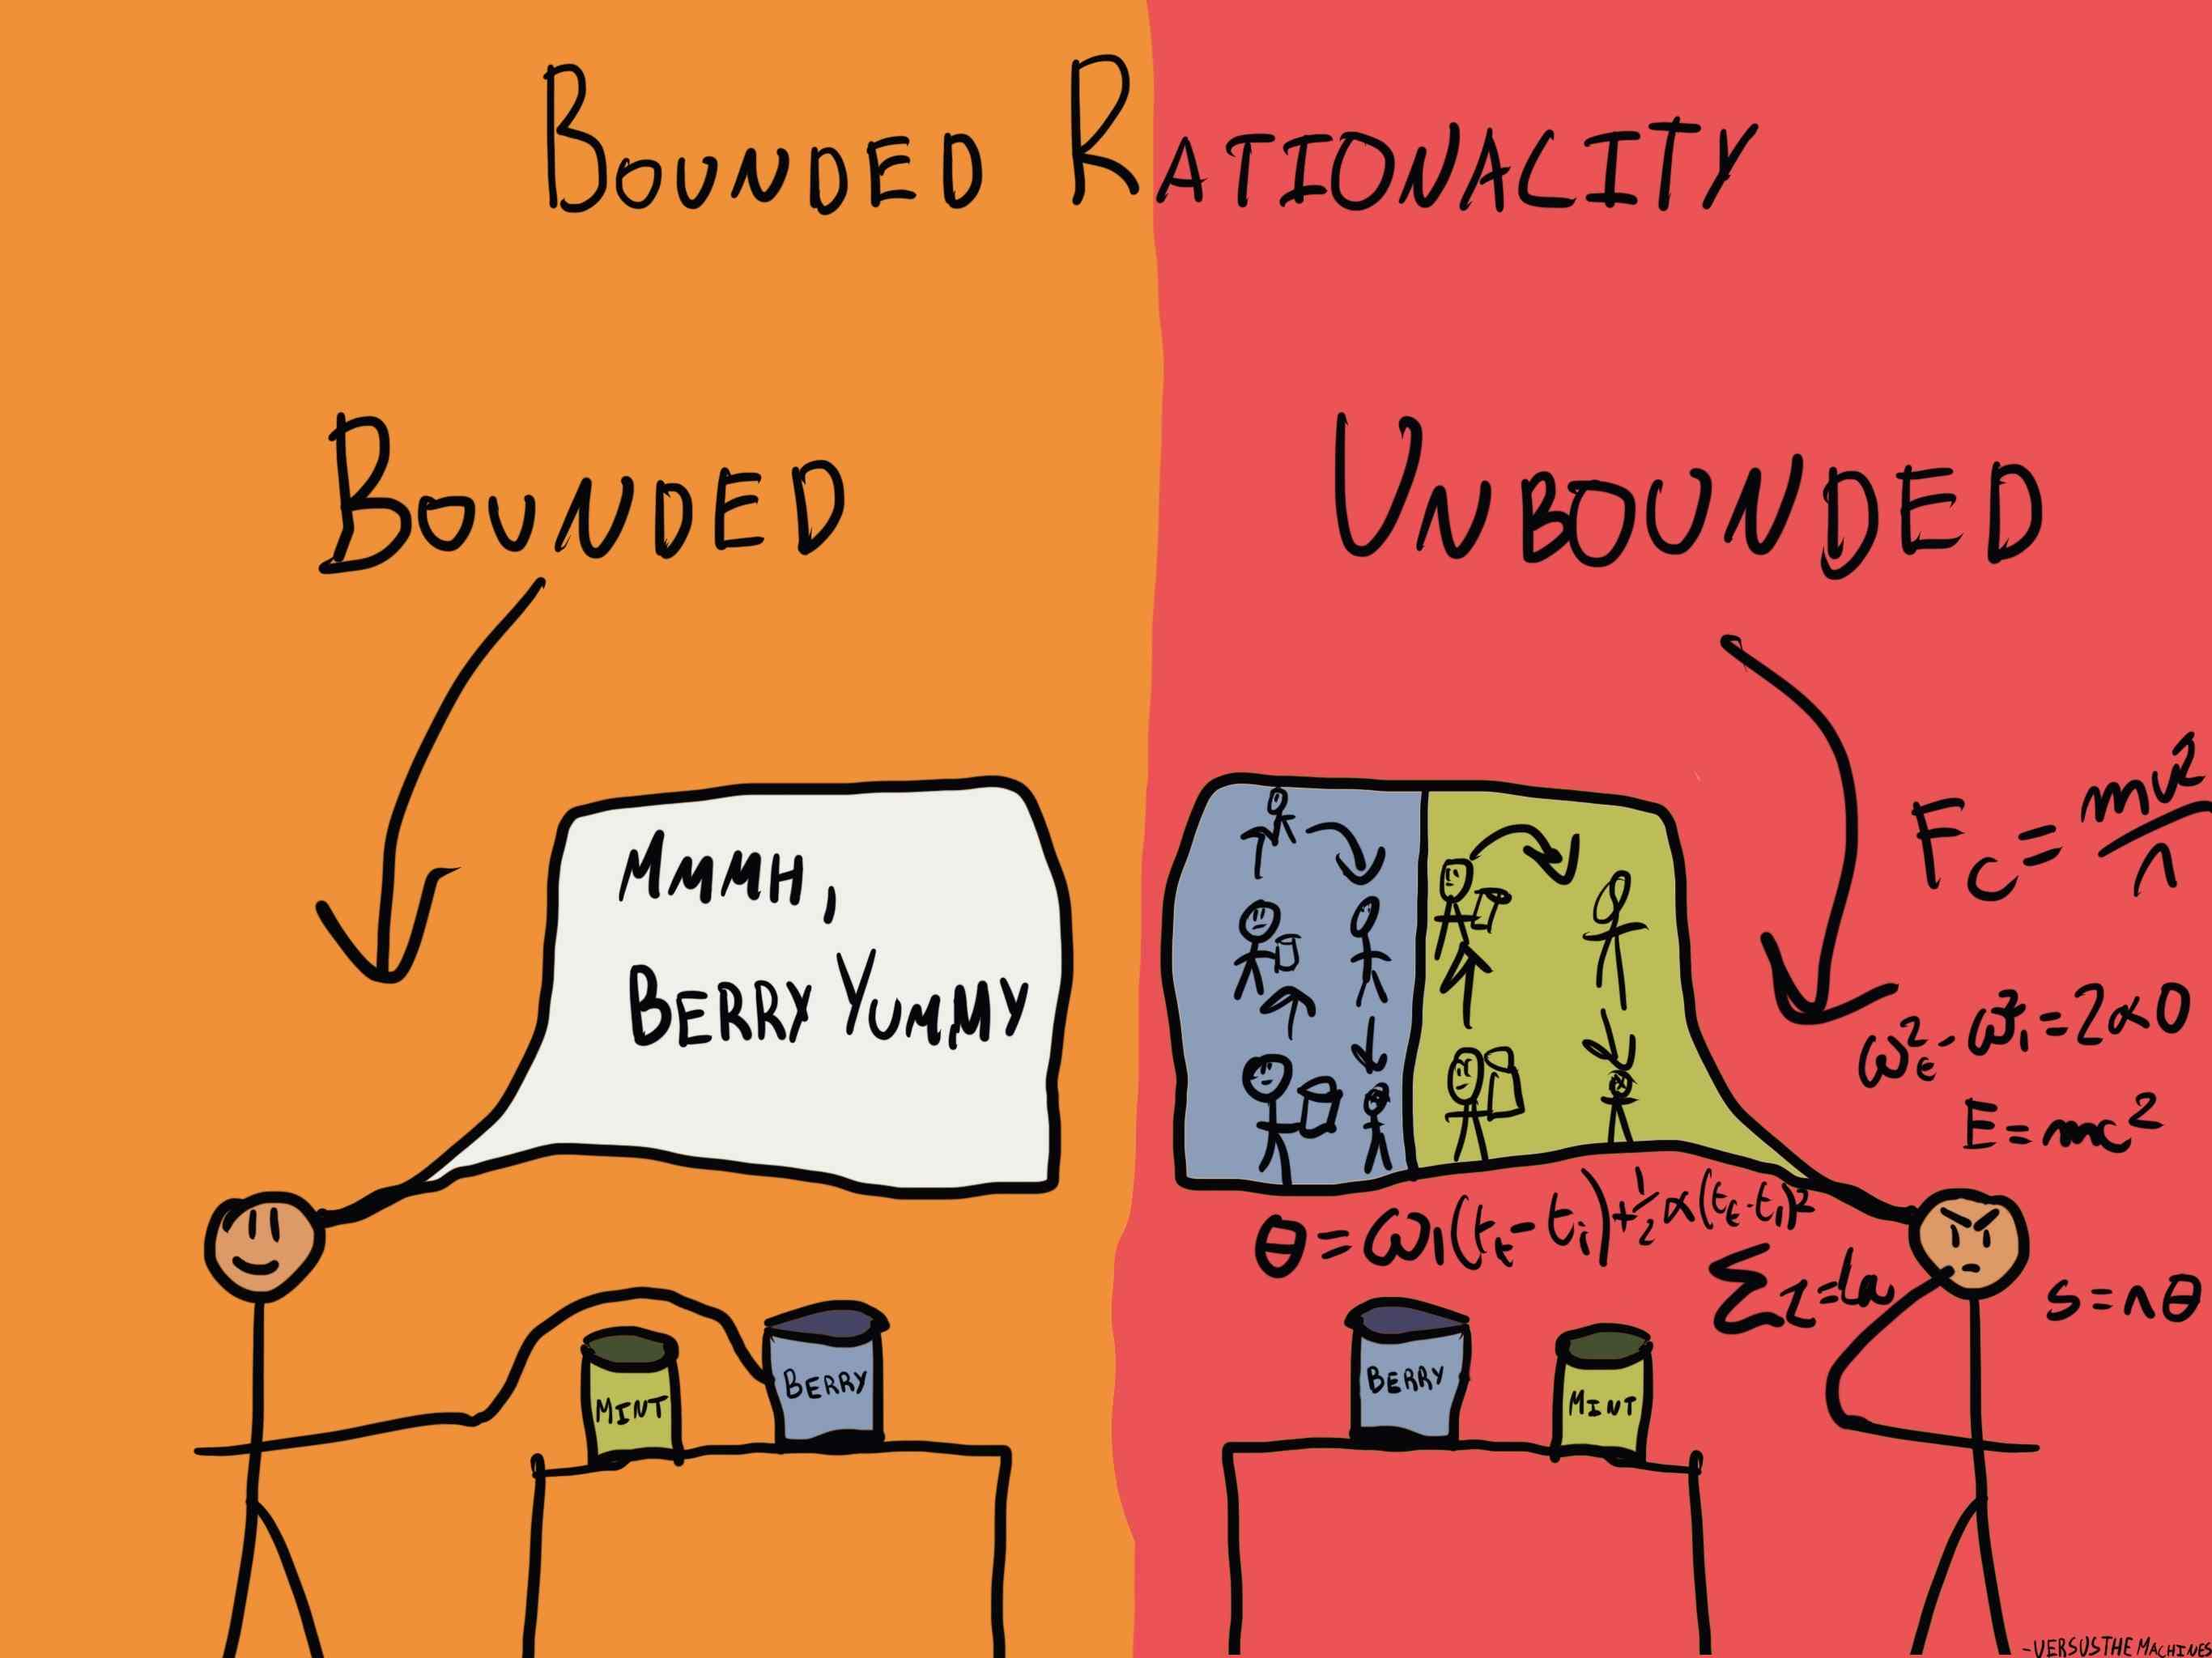
\includegraphics[width=0.5\textwidth,height=\textheight]{fig/bounded-rationality.jpg}
\caption[\label{fig:boundedrationality} Bounded rationality]{\label{fig:boundedrationality} Bounded rationality\footnotemark{}}
\end{figure}
\footnotetext{Picture is taken from \url{https://thedecisionlab.com/wp-content/uploads/2019/08/Bounded-Rationality.jpg}}

Bounded rationality proposes that decision making is constrained by managers' ability to process information, i.e., the rationally is \emph{bounded} (see figure \ref{fig:boundedrationality}). Managers use shortcuts and rules of thumb which are based on their prior experience with similar problems and scenarios. Given the constraints of managers in their position, they do not actually \emph{optimize} their choice given the available information. It is more like finding a \emph{satisfactory} solution, not necessarily the \emph{best} or the \emph{optimal} solution.

\begin{exercise}
\protect\hypertarget{exr:opti-sati}{}\label{exr:opti-sati}Optimal vs.~satisfactory solution

Using the images \ref{fig:picA} to \ref{fig:picD}, explain the idea of bounded rationality in the context of decision making.

\begin{figure}
\centering

\includegraphics[width=0.45\textwidth,height=\textheight]{fig/seeking.jpg}
\caption{\label{fig:picA} Picture A}
\end{figure}

\begin{figure}
\centering

\includegraphics[width=0.45\textwidth,height=\textheight]{fig/thumb.jpg}
\caption{\label{fig:picB} Picture B}
\end{figure}

\begin{figure}
\centering
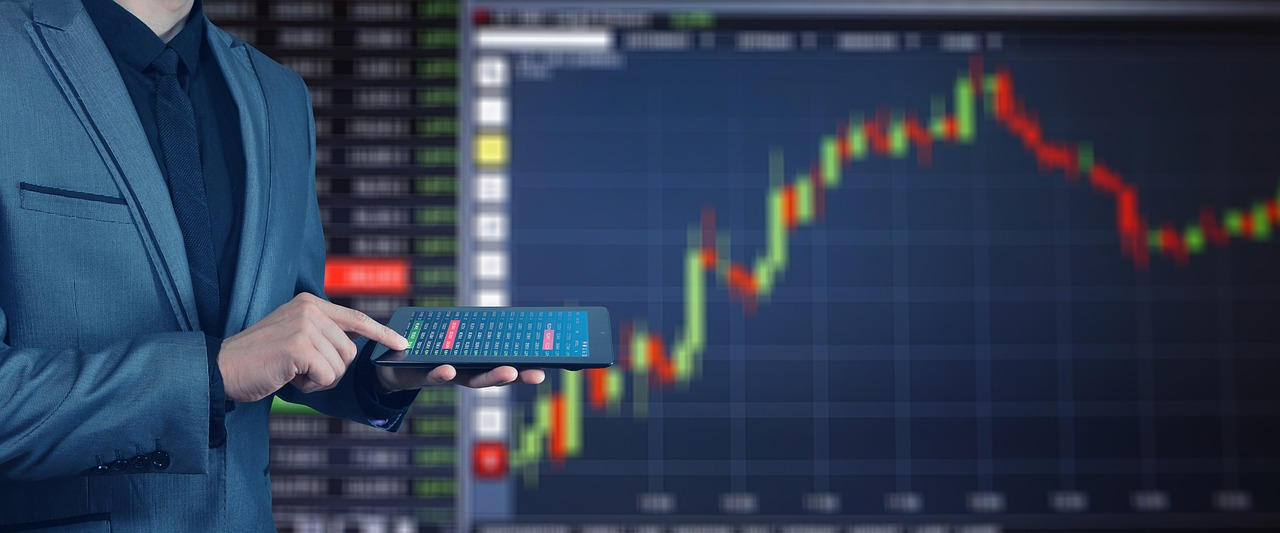
\includegraphics[width=0.45\textwidth,height=\textheight]{fig/stock.jpg}
\caption{\label{fig:picC} Picture C}
\end{figure}

\begin{figure}
\centering
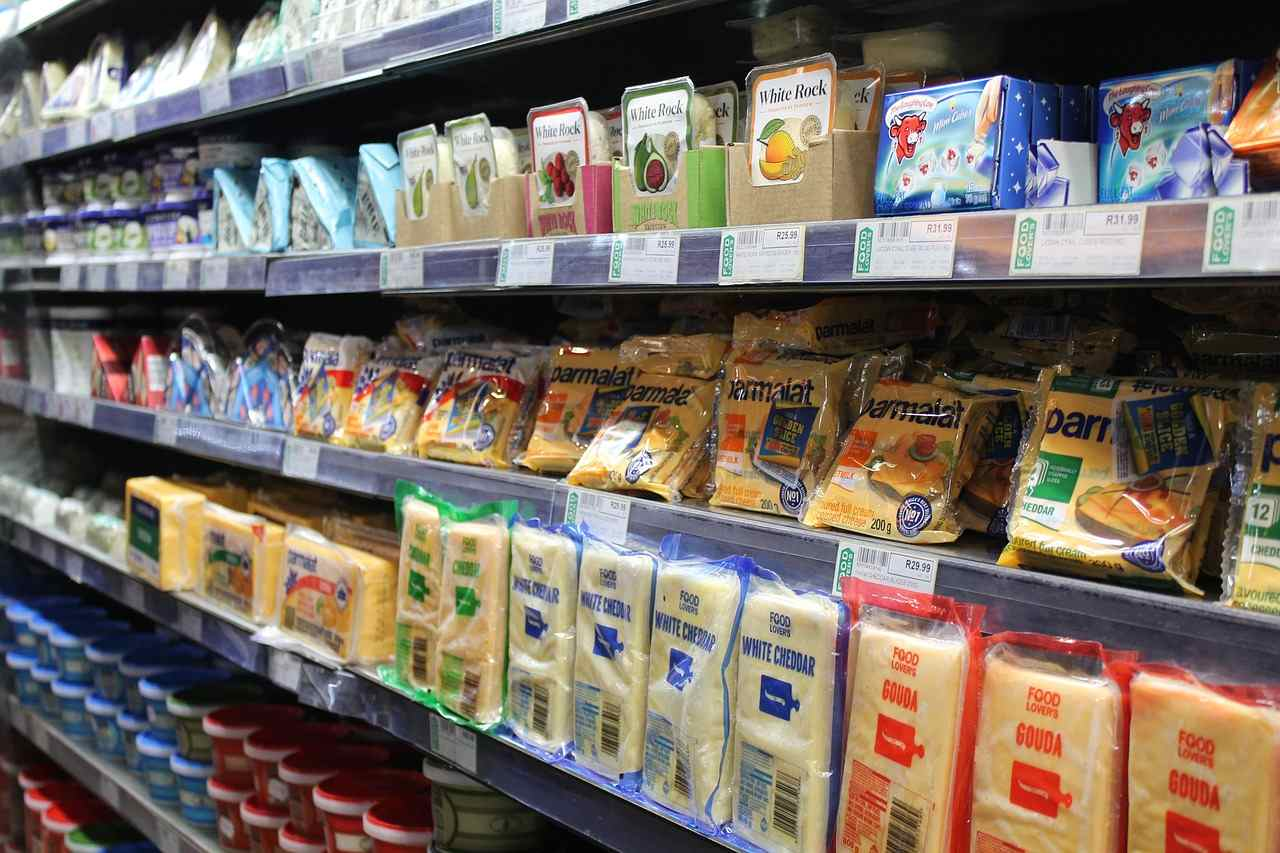
\includegraphics[width=0.45\textwidth,height=\textheight]{fig/supermarket.jpg}
\caption{\label{fig:picD} Picture D}
\end{figure}

Please find solution to the exercise \protect\hyperlink{sol:opti-sati}{in the appendix.}
\end{exercise}

\begin{exercise}
\protect\hypertarget{exr:irrational}{}\label{exr:irrational}

Are we irrational?

Discuss the following statement:

\begin{quote}
Since the rationality of individuals is bounded and it is obvious that individuals do not make optimal decisions, we can say that individuals act irrationally.
\end{quote}

\end{exercise}

\hypertarget{homo-economicus}{%
\section{Homo economicus}\label{homo-economicus}}

The so-called \emph{homo economicus} is often modeled by the assumption of perfect rationality. Actors are assumed to always act in a way that maximizes their utility (as consumers) and profit (as producers), and to this end they are capable of arbitrarily complex reasoning. That is, it is assumed that they are always capable of thinking through all possible outcomes and choosing the course of action that leads to the best possible outcome.

Of course, the assumption of \emph{homo economicus} is heroic, and I doubt that any serious economist has ever assumed that this assumption can be found one-to-one in reality. However, it is an assumption that helps to make predictions and explain the behavior of people and societies to some extent. I mean, what would happen if microeconomics went to the other extreme assuming irrationally acting individuals. The result would be, more or less, that we would not be able to make predictions and the future would be a random walk.

Nevertheless, economists and anyone who wants to make, apply, or think about economic theories should be aware of all the pitfalls that arise in our decision making and know that our ability to act rationally is limited. In real life, we often use heuristics to solve problems and make decisions.

A \textbf{heuristic} is any approach to solving a problem that uses a practical method that is not guaranteed to be optimal, perfect, or rational. However, a heuristic should--at best--be sufficient to achieve an immediate, short-term goal or approximation. Overall, people use heuristics because they either cannot act completely rationally or want to act rationally but do not have the time it would take to compute the perfect solution. Moreover, the effort is probably not worth it or simply not possible given the time constraints under which the problem must be solved.
A heuristic is a mental shortcut or rule of thumb to make decisions and solve problems quickly and efficiently. It helps individuals to arrive at a solution without extensive analysis or evaluation of all available information. Heuristics are usefull when time, resources, or information are limited.

While heuristics can be helpful in many situations, they can also lead to errors and biases, particularly when they are overused or misapplied. We will discuss some of these biases later on in greater detail.

\hypertarget{decision-trees}{%
\section{Decision trees}\label{decision-trees}}

When we decide under certain conditions, decision trees can be a helpful tool, as explained in \citep{Finne1998three}. If you want to know more about the use of decision trees I recommend reading \citet[ch.~4]{Bonanno2017Decision}.

\hypertarget{payoff-table}{%
\section{Payoff table}\label{payoff-table}}

A payoff table, also known as a decision matrix, can be a helpful tool for decision making, as shown in the table below. It presents the available alternatives denoted by \(A_i\), along with the possible future states of nature or goals denoted by \(N_j\).

The payoff or outcome depends on both the chosen alternative and the future state of nature that occurs. For instance, if alternative \(A_i\) is chosen and state of nature \(N_j\) occurs, the resulting payoff is \(O_{ij}\). Our goal is to choose the alternative \(A_i\) that yields the most favorable outcome \(O_{ij}\).

\begin{longtable}[]{@{}
  >{\raggedright\arraybackslash}p{(\columnwidth - 12\tabcolsep) * \real{0.3143}}
  >{\raggedright\arraybackslash}p{(\columnwidth - 12\tabcolsep) * \real{0.1571}}
  >{\raggedright\arraybackslash}p{(\columnwidth - 12\tabcolsep) * \real{0.1000}}
  >{\raggedright\arraybackslash}p{(\columnwidth - 12\tabcolsep) * \real{0.1143}}
  >{\raggedright\arraybackslash}p{(\columnwidth - 12\tabcolsep) * \real{0.1143}}
  >{\raggedright\arraybackslash}p{(\columnwidth - 12\tabcolsep) * \real{0.1143}}
  >{\raggedright\arraybackslash}p{(\columnwidth - 12\tabcolsep) * \real{0.0857}}@{}}
\caption{Payoff matrix}\tabularnewline
\toprule()
\endhead
State of nature (N) & \(N_1\) & \(N_2\) & \(\cdots\) & \(N_j\) & \(\cdots\) & \(N_n\) \\
Probability (p) & \(p_1\) & \(p_2\) & \(\cdots\) & \(p_j\) & \(\cdots\) & \(p_n\) \\
Alternative (A) & & & & & & \\
\(A_1\) & \(O_{11}\) & \(O_{12}\) & \(\cdots\) & \(O_{1j}\) & \(\cdots\) & \(O_{1n}\) \\
\(A_2\) & \(O_{21}\) & \(O_{22}\) & \(\cdots\) & \(O_{2j}\) & \(\cdots\) & \(O_{2n}\) \\
\(\cdots\) & \(\cdots\) & \(\cdots\) & \(\cdots\) & \(\cdots\) & \(\cdots\) & \(\cdots\) \\
\(A_i\) & \(O_{i1}\) & \(O_{i2}\) & \(\cdots\) & \(O_{ij}\) & \(\cdots\) & \(O_{in}\) \\
\(\cdots\) & \(\cdots\) & \(\cdots\) & \(\cdots\) & \(\cdots\) & \(\cdots\) & \(\cdots\) \\
\(A_m\) & \(O_{m1}\) & \(O_{m2}\) & \(\cdots\) & \(O_{mj}\) & \(\cdots\) & \(O_{mn}\) \\
\bottomrule()
\end{longtable}

If we assume that all objectives are independent from each other and that we are certain about the state of nature, the decision is rather trivial: just go for the alternative with the best outcome for each state of nature. However, most real-world scenarios are not that simple because most states of nature are more complex and needs further to be considered.

\hypertarget{review}{%
\section{Review}\label{review}}

\begin{itemize}
\tightlist
\item
  Decision analysis is about using information in order to come to a decision.
\item
  A structured and rational process can help improve the chances of receiving good decision outcomes.
\item
  As decision problems are often (too) complex to fully capture or solve rationally. Thus, a good decision analysis should try to use the available information and the existing understanding of the problem as transparent, consistent, and logical as possible.
\item
  A complex decision problem should be simplified and hence decomposed into its basic and most important components.
\item
  There are hundred of different \emph{schemes} or \emph{strategies} how to make decisions in certain circumstances. Many heuristics exist how to think, behave, and calculate to come to a wise decision.
\item
  Mostly decisions are based on subjective expectations. These expectations are difficult to validate.
\item
  Articulating exact expectation and preferences is a difficult task and the information that stems from these articulation is full of biases. Decision analytic tools need to take that into consideration.
\end{itemize}

\begin{exercise}
\protect\hypertarget{exr:lisapregnant}{}\label{exr:lisapregnant}Lisa is pregnant

The following question stems from a study carried out by \citet{Kahneman1972Subjective}: Lisa is thirty-three and is pregnant for the first time. She is worried about birth defects such as Down syndrome. Her doctor tells her that she need not worry too much because there is only a 1 in 1,000 chance that a woman of her age will have a baby with Down syndrome. Nevertheless, Lisa remains anxious about this possibility and decides to obtain a test, known as the Triple Screen, that can detect Down syndrome. The test is moderately accurate: When a baby has Down syndrome, the test delivers a positive result 86 percent of the time. There is, however, a small `false positive' rate: 5 percent of babies produce a positive result despite not having Down syndrome. Lisa takes the Triple Screen and obtains a positive result for Down syndrome.

Given this test result, what are the chances that her baby has Down syndrome?

\begin{enumerate}
\def\labelenumi{\alph{enumi})}
\tightlist
\item
  0-20 percent chance
\item
  21-40 percent chance
\item
  41-60 percent chance
\item
  61-80 percent chance
\item
  81-100 percent chance
\end{enumerate}

Think about the question and put your answer here:

\url{https://pingo.coactum.de/} Code: 666528

Please find solution to the exercise \protect\hyperlink{sol:lisapregnant}{in the appendix.}
\end{exercise}

\hypertarget{decision-making-theory}{%
\chapter{Decision making theory}\label{decision-making-theory}}

\hypertarget{decision-making-under-certainty}{%
\section{Decision making under certainty}\label{decision-making-under-certainty}}

\begin{center}\rule{0.5\linewidth}{0.5pt}\end{center}

After successful completion of the module, students are able to:

\begin{itemize}
\tightlist
\item
  Distinguish different theories of decision making.
\item
  Calculate the optimal decision under certainty, uncertainty, and under risk.
\item
  Describe and use various criteria of decision making.
\item
  Simplify complex decision making situations and use formal approaches of decision making to guide the decision making behavior of managers.
\end{itemize}

\begin{center}\rule{0.5\linewidth}{0.5pt}\end{center}

Decision making under certainty means that we assume that we are certain about the future state of nature, i.e., we have complete information about the alternative actions and their consequences. Making decisions under certainty may seem like a trivial exercise. However, many problems are so complex that sophisticated mathematical techniques are sometimes needed to find the best solution.

\hypertarget{decision-making-with-complex-state-of-natures}{%
\subsection{Decision making with complex state of natures}\label{decision-making-with-complex-state-of-natures}}

Suppose you have to decide between four different restaurants where you want to go out to eat (\(a_1\), \(a_2\), \(a_3\), \(a_4\)). The restaurants have different characteristics such as the quality of the food k1, the quality of the music played \(k_2\), the price \(k_3\), the quality of the service \(k_4\), and the environment \(k_5\). The corresponding payoff table is given below. High numbers represent good quality. In other words, \(a_i\) refer to competing alternatives where to eat for dinner, and \(k_i\) are certain characteristics of the respective restaurant, and the numbers given in the table indicate the output.

\begin{longtable}[]{@{}cccccc@{}}
\caption{Weighting scheme}\tabularnewline
\toprule()
& \(k_1\) & \(k_2\) & \(k_3\) & \(k_4\) & \(k_5\) \\
\midrule()
\endfirsthead
\toprule()
& \(k_1\) & \(k_2\) & \(k_3\) & \(k_4\) & \(k_5\) \\
\midrule()
\endhead
\(a_1\) & 3 & 0 & 7 & 1 & 4 \\
\(a_2\) & 4 & 1 & 4 & 2 & 1 \\
\(a_3\) & 4 & 0 & 3 & 2 & 1 \\
\(a_4\) & 5 & 1 & 2 & 3 & 1 \\
\bottomrule()
\end{longtable}

\hypertarget{domination}{%
\subsection*{Domination}\label{domination}}

Some alternative can be excluded because they are \textbf{dominated} by other alternatives. In the scheme above you can see that alternative 2 is always superior to alternative 3, i.e., alternative 3 is dominated by alternative 2. Thus, it does not make sense to think about alternative 3:

\begin{longtable}[]{@{}cccccc@{}}
\caption{Alternative 3 is dominated by alternative 2}\tabularnewline
\toprule()
& \(k_1\) & \(k_2\) & \(k_3\) & \(k_4\) & \(k_5\) \\
\midrule()
\endfirsthead
\toprule()
& \(k_1\) & \(k_2\) & \(k_3\) & \(k_4\) & \(k_5\) \\
\midrule()
\endhead
\(a_1\) & 3 & 0 & 7 & 1 & 4 \\
\(a_2\) & 4 & 1 & 4 & 2 & 1 \\
\(a_3\) & \sout{4} & \sout{0} & \sout{3} & \sout{2} & \sout{1} \\
\(a_4\) & 5 & 1 & 2 & 3 & 1 \\
\bottomrule()
\end{longtable}

\hypertarget{weighting}{%
\subsection*{Weighting}\label{weighting}}

As the objectives \(k_j\) of the scheme above do not represent different states of nature but represent characteristics and its corresponding utility (whatever that number may mean in particular) of one particular characteristics if we choose a respective alternative. For example, think of that you can choose one out of four restaurants, \(a_1,\dots,a_4\), in order to eat a five-course menu, \(k_1,\dots,k_5\), and the outcome represents your utility of each course, \(j\), for each restaurant, \(i\). We already know from the domination principle that restaurant \(a_3\) is a bad choice.

Suppose you have a preference for the first three courses. Specifically, suppose that your preference scheme is as follows:

\[
g_1 : g_2 : g_3 : g_4 : g_5 = 3 : 4 : 3 : 1 : 1
\]

This means, for example, that you value the second food course four times more than the last course.

\[
w_1=3/12; w_2=4/12; w_3=3/12; w_4 = w_5 =1/12.
\]

In order to find a decision criteria you can calculate the aggregated expected utility as follows:

\[
\Phi(a_i)=\sum_{p=1}^{r}w_p\cdot u_{ip} \rightarrow max
\]

The results are as follows:

\begin{longtable}[]{@{}ccccccc@{}}
\toprule()
& \(k_1\) & \(k_2\) & \(k_3\) & \(k_4\) & \(k_5\) & \(\Phi(a_i)\) \\
\midrule()
\endhead
\(a_1\) & 3 & 0 & 7 & 1 & 4 & 35//12 \\
\(a_2\) & 4 & 1 & 4 & 2 & 1 & 31//12 \\
\(a_3\) & 4 & 0 & 3 & 2 & 1 & 24//12 \\
\(a_4\) & 5 & 1 & 2 & 3 & 1 & 29//12 \\
\bottomrule()
\end{longtable}

Thus, \(a_1\succ a_2 \succ a_4 \succ a_3\), i.e., you prefer alternative \(a_1\).

\hypertarget{preferences-and-decision-criteria}{%
\subsection*{Preferences and decision criteria}\label{preferences-and-decision-criteria}}

Maybe not all courses play the same role for you so you can take your decision based on your preference scheme. For example, assume some courses are more important to you than others such as \(k_1 \succ k_3 \succ k_2 \succ k_4 \succ k_5\). Now, if you decide based on your most important course you should choose restaurant 4 because this gives you the highest utility in that dish. If you further assume that you are not that hungry and you only like to have two dishes, then you should probably better go for restaurant 1 because the aggregated utility in the two preferred courses is 10 utility units and restaurants 2, 3 and 4 can only offer 8, 7 and 7 utility units in your two preferred courses.

\hypertarget{kuxf6rths-maximin-rule}{%
\subsection*{Körth's Maximin-Rule}\label{kuxf6rths-maximin-rule}}

According to this rule, we compare alternatives by the worst possible outcome under each alternative, and we should choose the one which maximizes the utility of the worst outcome. More concrete, the procedure consists of 4 steps:

\begin{enumerate}
\def\labelenumi{\arabic{enumi}.}
\tightlist
\item
  Calculate the utility maximum for each column of the payoff matrix: \[\overline{O}j=\max{i=1,\dots,m}{O_{ij}}\qquad \forall j.\]
\item
  Calculate for each cell the relative utility, \[\frac{O_{ij}}{\overline{O}_j}.\]
\item
  Calculate for each row the minimum: \[\Phi(a_i)=\min_{j=1,\dots,p}\left(\frac{O_{ij}}{\overline{O}_j}\right).\]
\item
  Set preferences by maximizing \(\Phi(a_i)\).
\end{enumerate}

\hypertarget{linear-programming}{%
\subsection{Linear programming}\label{linear-programming}}

Linear Programming is a common technique for decision making under certainty. It allows to express a desired benefit (such as profit) as a mathematical function of several variables. The solution is the set of values for the independent variables (decision variables) that serves to maximize the benefit or to minimize the negative outcome under consideration of certain limits, a.k.a. constraints. The method usually follows a four step procedure:

\begin{enumerate}
\def\labelenumi{\arabic{enumi}.}
\tightlist
\item
  state the problem;
\item
  state the decision variables;
\item
  set up an objective function;
\item
  clarify the constraints.
\end{enumerate}

\textbf{Example:}
Consider a factory producing two products, product X and product Y. The problem is this: If
you can realize \$10.00 profit per unit of product X and \$14.00 per unit of product Y, what is the production level of x units of product X and y units of product Y that maximizes the profit P each day? Your production, and therefore your profit, is subject to resource limitations, or constraints. Assume in this example that you employ five workers---three machinists and two assemblers---and that each works only 40 hours a week.\footnote{The example is taken from \citet[p.~134f]{Morse2014Managing}.}

\begin{itemize}
\tightlist
\item
  Product X requires three hours of machining and one hour of assembly per unit.
\item
  Product Y requires two hours of machining and two hours of assembly per unit.
\end{itemize}

\begin{enumerate}
\def\labelenumi{\arabic{enumi}.}
\tightlist
\item
  \emph{State the problem:} How many of product X and product Y to produce to maximize profit?
\item
  \emph{Decision variables:} Suppose x denotes the number of product X to produce per day and y denotes number of product Y to produce per day
\item
  \emph{Objective function:} Maximize \[P = 10x + 14y\]
\item
  \emph{Constraints:}
\end{enumerate}

\begin{itemize}
\tightlist
\item
  machine time=120h
\item
  assembling time=80h
\item
  hours needed for production of one good:
\end{itemize}

\emph{machine time:} \(x\rightarrow 3h\) and \(y \rightarrow 2h\)

\emph{assembling time:} \(x\rightarrow 1h\) and \(y \rightarrow 2h\)

Thus, we get:
\[3x + 2y \leq 120 \quad \Leftrightarrow y\leq 60-\frac{3}{2}x \quad \text{(hours of machining time)}\]
\[x + 2y \leq 80 \quad \Leftrightarrow y \leq 40-\frac{1}{2}x \quad \text{(hours of assembly time)}\]
Since there are only two products, these limitations can be shown on a two-dimensional graph (\ref{fig:lpe2}). Since all relationships are linear, the solution to our problem will fall at one of the corners.

\begin{figure}
\centering
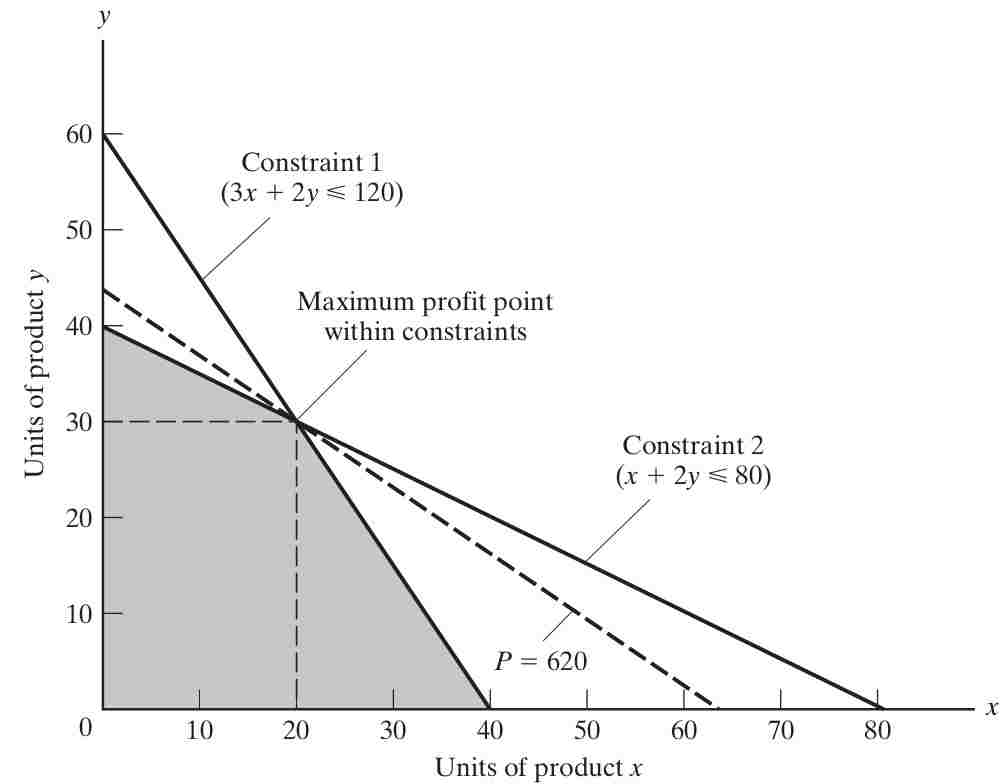
\includegraphics[width=0.75\textwidth,height=\textheight]{fig/lpe2.jpg}
\caption{\label{fig:lpe2} Linear program example: constraints and solution}
\end{figure}

To draw the isoprofit function in a plot with the good \(y\) on the y-axis and good \(x\) on the x-axis, we can re-arrange the objective function to get \[y=\frac{1}{14}P-\frac{10}{14}x\]
To illustrate the function let us consider some arbitrarily chosen levels of profit in \autoref{fig:lpe}:

\begin{itemize}
\tightlist
\item
  \$350 by selling 35 units of X or 25 units of Y
\item
  \$700 by selling 70 units of X or 50 units of Y
\item
  \$620 by selling 62 units of X or 44.3 units of Y.
\end{itemize}

\begin{figure}
\centering
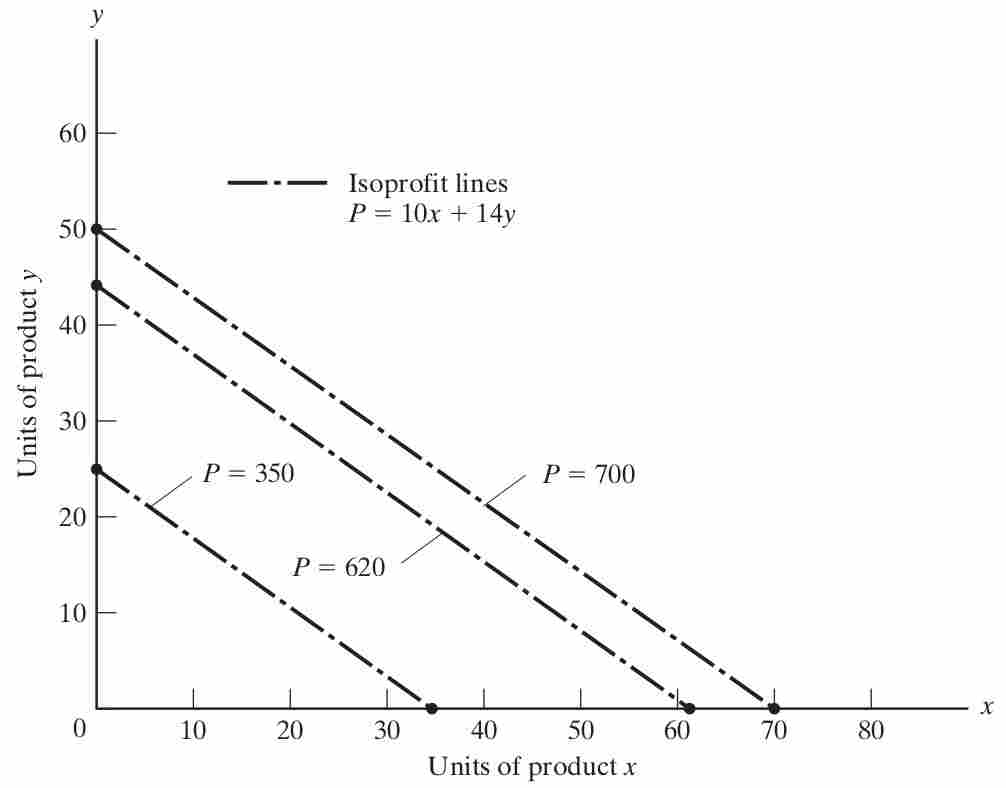
\includegraphics[width=0.75\textwidth,height=\textheight]{fig/lpe.jpg}
\caption{\label{fig:lpe} Linear program example: isoprofit lines}
\end{figure}

To find the solution, begin at some feasible solution (satisfying the given constraints) such as \((x,y) = (0,0)\), and proceed in the direction of \emph{steepest ascent} of the profit function (in this case, by increasing production of Y at \$14.00 profit per unit) until some constraint is reached. Since assembly hours are limited to 80, no more than 80/2, or 40, units of Y can be made, earning \(40 \cdot \$14.00\), or \$560 profit. Then proceed along the steepest allowable ascent from there (along the assembly constraint line) until another constraint (machining hours) is reached. At that point, (x,y) = (20,30) and profit P = (20 * +10.00) + (30 * +14.00), or \$620. Since there is no remaining edge along which profit increases, this is the optimum solution.

\begin{exercise}
\protect\hypertarget{exr:koerth-example}{}\label{exr:koerth-example}Körth: example

For the following payoff-matrix, calculate the order of preferences based on the Körth-rule.

\begin{longtable}[]{@{}llllll@{}}
\toprule()
\(O_{ij}\) & \(k_1\) & \(k_2\) & \(k_3\) & \(k_4\) & \(k_5\) \\
\midrule()
\endhead
\(a_1\) & 3 & 0 & 7 & 1 & 4 \\
\(a_2\) & 4 & 0 & 4 & 2 & 1 \\
\(a_3\) & 4 & -1 & 3 & 2 & 1 \\
\(a_4\) & 5 & 1 & 3 & 3 & 1 \\
\bottomrule()
\end{longtable}

Please find solution to the exercise \protect\hyperlink{sol:koerth-example}{in the appendix.}
\end{exercise}

\hypertarget{lagrange-multiplier-method}{%
\subsection{Lagrange Multiplier Method}\label{lagrange-multiplier-method}}

\begin{figure}
\centering
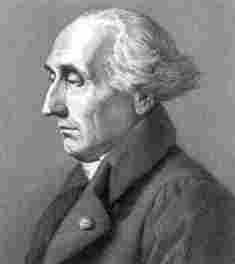
\includegraphics[width=0.25\textwidth,height=\textheight]{fig/Lagrange.jpg}
\caption{\label{fig:Lagrange} Joseph-Louis
Lagrange (1736-1813)}
\end{figure}

The Lagrange Multiplier Method is a mathematical technique that goes back to Joseph-Louis Lagrange (see figure \ref{fig:Lagrange}. It is often used in optimization problems involving constraints. In decision making, this method can be used to determine the optimal values of decision variables subject to certain constraints.

\begin{figure}
\centering
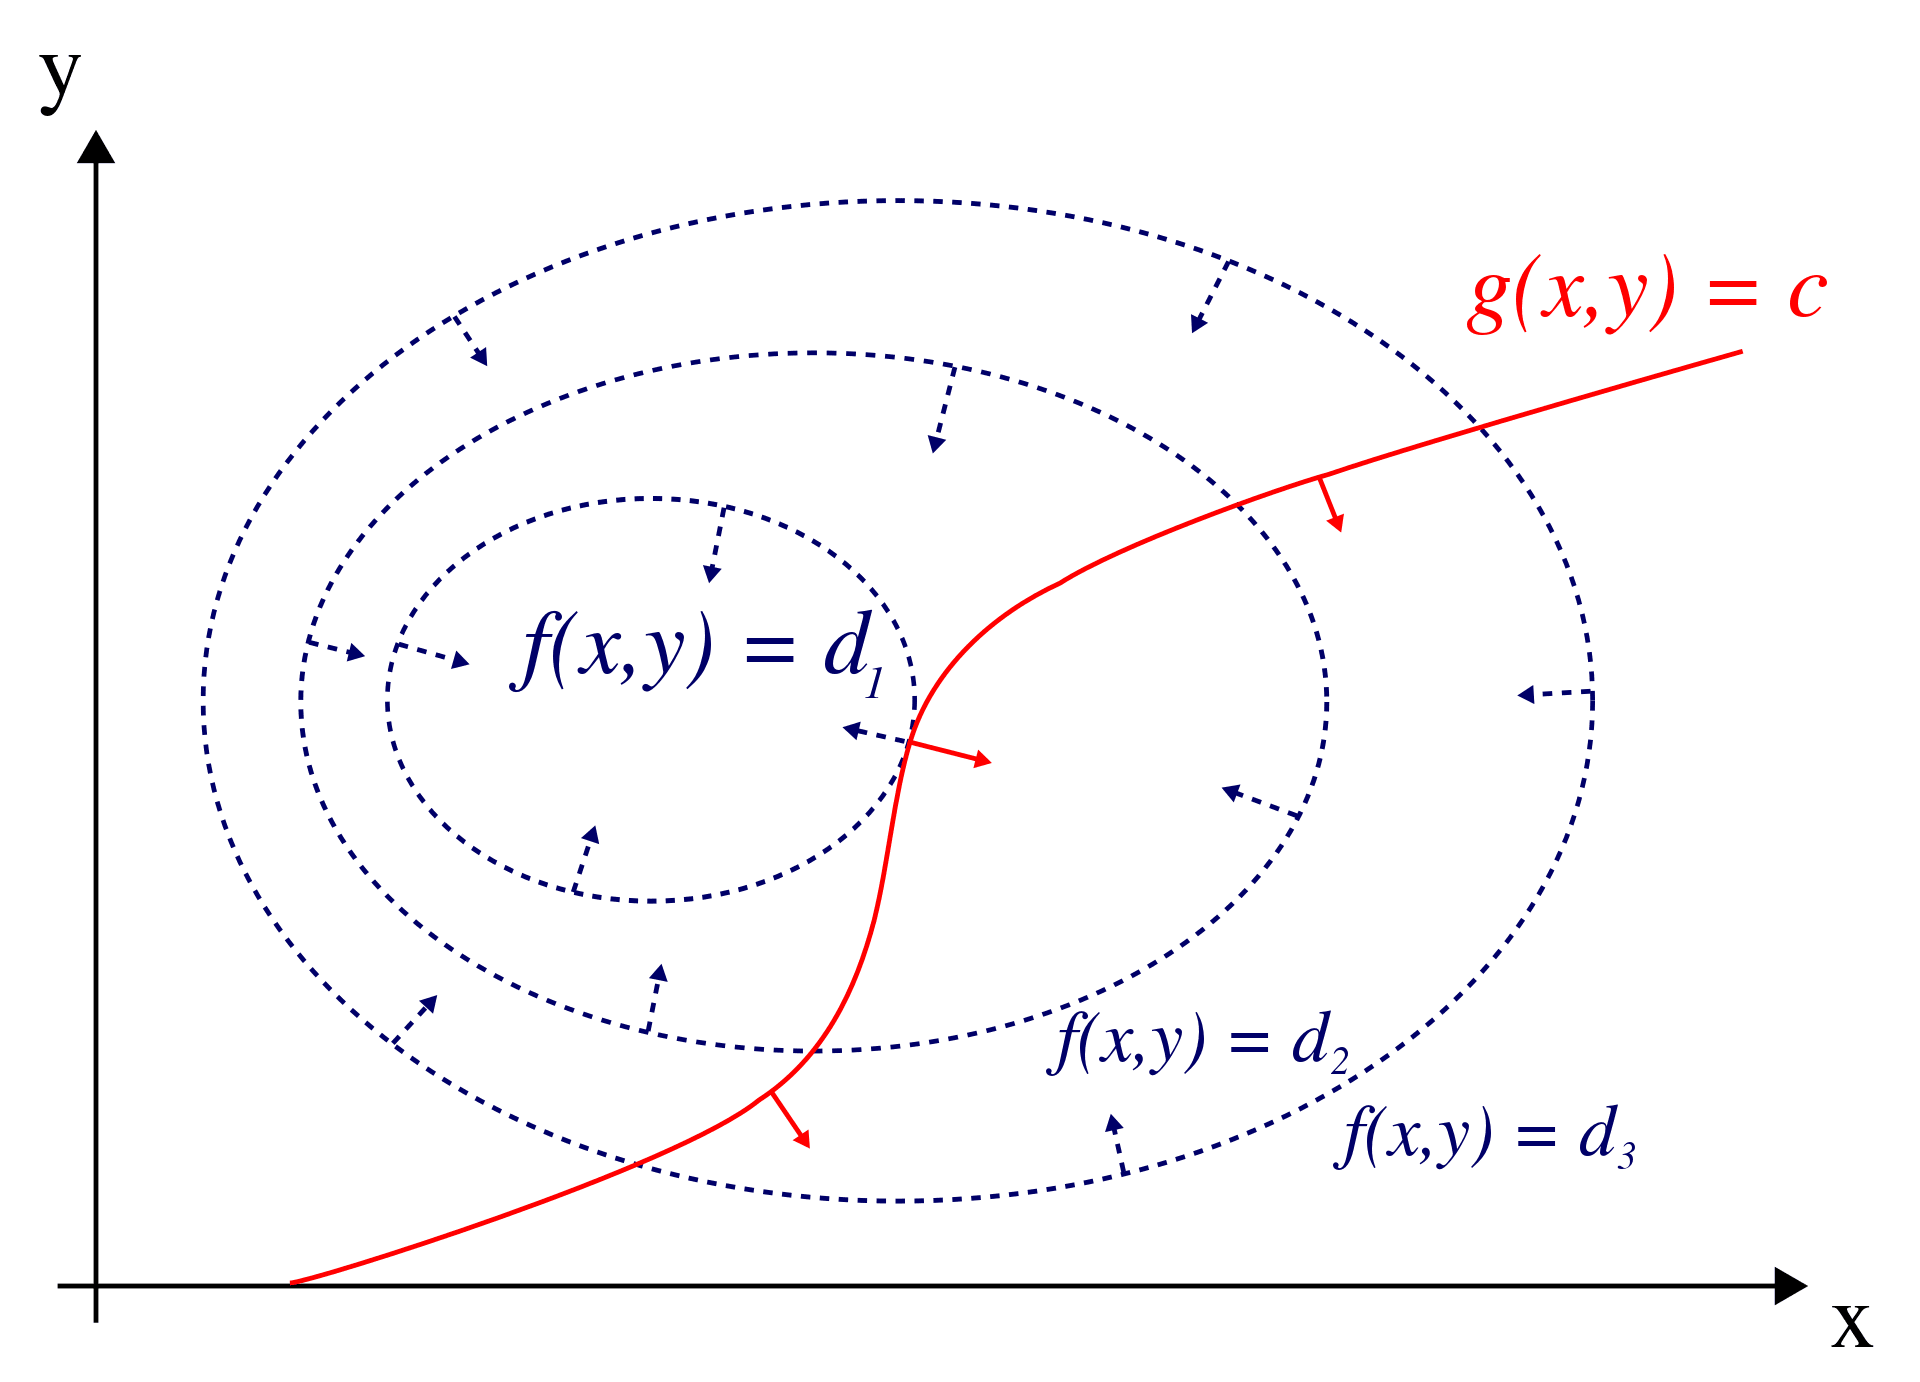
\includegraphics[width=0.5\textwidth,height=\textheight]{fig/lagr2.png}
\caption{\label{fig:lagr2} The Lagrange method}
\end{figure}

The basic idea behind the Lagrange Multiplier Method is to introduce additional variables, called Lagrange multipliers, to the problem. These multipliers allow us to convert the constraints into equations that can be used to find the optimal values of the decision variables. The method is a strategy for finding the local maxima and minima of a function subject to constraints like stylized in figure \ref{fig:lagr2}. The red curve shows the constraint \(g(x, y) = c\). The blue curves are contours of \(f(x, y)\). The point where the red constraint tangentially touches a blue contour is the maximum of \(f(x, y)\) along the constraint, since \(d1 > d2\).\footnote{For a detailed mathematical explanation, feel free to watch Aviv Censor's video \url{https://youtu.be/AxEVJoxv-Z8}.}
An intuitive explanation of the method can is provided in the video of Trefor Bazett: \url{https://youtu.be/8mjcnxGMwFo}

The method can be describe in four steps:

\textbf{Step 1: The problem to be solved}

The problem that we want to solve can be written in the following way,
\[\begin{array}{ll}
\max _{x, y} & F(x, y) \\
\text { s.t. } & g(x, y)=0
\end{array}\] where \(F(x, y)\) is the function to be maximized and
\(g(x, y)=0\) is the constraint to be respected. Notice that
\(\max _{x, y}\) means that we must solve (maximize) with respect to \(x\) and \(y\).

\textbf{Step 2: Define the Lagrangian Multiplier}

Define a new function, the \emph{Lagrangian} \(\mathcal{L}\), by combining the two functions of the problem and adding the new variable \(\lambda\). The \(\lambda\) is called the \emph{Lagrange Multiplier}.
\[\mathcal{L}(x, y, \lambda)=F(x, y)+\lambda g(x, y)\]

\textbf{Step 3: Find the first order conditions}

Differentiate \(\mathcal{L}\) w.r.t. \(x, y,\) and \(\lambda\) and equate the partial derivatives to 0: \[\begin{aligned}
\frac{\partial \mathcal{L}(x, y, \lambda)}{\partial x}=0 & \Leftrightarrow \frac{\partial F(x, y)}{\partial x}+\lambda \frac{\partial g(x, y)}{\partial x}=0 \\
\frac{\partial \mathcal{L}(x, y, \lambda)}{\partial y}=0 & \Leftrightarrow \frac{\partial F(x, y)}{\partial y}+\lambda \frac{\partial g(x, y)}{\partial y}=0 \\
\frac{\partial \mathcal{L}(x, y, \lambda)}{\partial \lambda}=0 & \Leftrightarrow g(x, y)=0\end{aligned}\]

\textbf{Step 4: Solve the system of equations}

The solution to the system of three equations above gives the required optimal quantities.

\begin{exercise}
\protect\hypertarget{exr:burger}{}\label{exr:burger}Burgers and drinks

Suppose you are in a fast food restaurant and you want to buy burgers and some drinks. You have €12 to spend, a burger costs €3 and a drink costs €2.

\begin{enumerate}
\def\labelenumi{\alph{enumi})}
\item
  Assume that you want to spend all your money and that you can only buy complete units of each products. What are the possible choices of consumption?
\item
  Given your utility function \(U(x,y)=B^{0.6}D^{0.4}\) calculate for each possible consumption point your overall utility. How will you decide?
\item
  Assume that you want to spend all your money and that both products can be bought on a metric scale where one burger weights 200 grams and a drink is 200 ml. How much of both goods would you consume now?
\end{enumerate}

\emph{Hint: Use the Lagrangian multiplier method.}*\footnote{Also see: \url{http://www.sfu.ca/~wainwrig/5701/notes-lagrange.pdf}}

Please find solution to the exercise \protect\hyperlink{sol:burger}{in the appendix.}
\end{exercise}

\begin{exercise}
\protect\hypertarget{exr:consumptionlagr}{}\label{exr:consumptionlagr}Consumption choice

Consumption Choice Suppose you want to spend your complete budget of €30, \[I=30,\] on the consumption of two goods, \(A\) and \(B\). Further assume good \(A\) costs €6, \[p_A=6,\] and good \(B\) costs €4, \[p_B=4\] and that you want to maximize your utility that stems from consuming the two goods. Calculate how much of both goods to buy and consume, respectively, when your utility function is given as \[U(A,B)=A^{0.8}B^{0.2}\]
\end{exercise}

\begin{exercise}
\protect\hypertarget{exr:costlagr}{}\label{exr:costlagr}Cost-minimizing combination of factors

Using two input factors \(r_1\) and \(r_2\), a firm wants to produces a fixed quantity of a product, that is \(x=20\). Given the production function \[x=\frac{5}{4} r_1^{\frac{1}{2}} r_2^{\frac{1}{2}}\] and the factor prices \[p_{r_1}=1 \quad \text{ and } p_{r_2}=4.\] calculate the cost-minimizing combination of factors (\(r_1, r_2\)).
\end{exercise}

\begin{exercise}
\protect\hypertarget{exr:derilagr}{}\label{exr:derilagr}Derivation of demand function

A representative consumer has on average the following utility function: \(U=x y,\) and faces a budget constraint of \(B=P_{x} x+P_{y} y,\) where \(B, P_{x}\) and \(P_{y}\) are the budget and prices, which are given. Solve the following choice problem:

Maximize \(U=x y\) s.t. \(B=P_{x} x+P_{y} y\).
\end{exercise}

\begin{exercise}
\protect\hypertarget{exr:cddlagr}{}\label{exr:cddlagr}Cobb-Douglas and demand

A consumer who has a Cobb-Douglas utility function \(u(x, y)=A x^{\alpha} y^{\beta}\) faces the budget constraint \(p x+q y=I\), where \(A, \alpha, \beta, p,\) and \(q\) are positive constants. Solve the consumer`s problem: \[\begin{array}{lll} \max A x^{\alpha} y^{\beta} & \text { subject to } & p x+q y=I \end{array}\]
\end{exercise}

\begin{exercise}
\protect\hypertarget{exr:lagrcons}{}\label{exr:lagrcons}Lagrange with n-constraints

Write down the Lagrangian multiplier for the following minimization problem:

Minimize \(f(\mathbf{x})\) subject to:
\[\begin{aligned}
    g_1(\mathbf{x})&=0 \\
    g_2(\mathbf{x})&=0\\
    &\vdots\\
    g_n(\mathbf{x})&=0,\end{aligned}\]
where \(n\) denotes the number of constraints.
\end{exercise}

\hypertarget{decision-making-under-uncertainty}{%
\section{Decision making under uncertainty}\label{decision-making-under-uncertainty}}

When it comes to decision-making under uncertainty you need to have a criterion that helps you to come to a \emph{rational} decision. The choice of criteria is a matter of taste and should at best fit with overall (business) strategy.

\hypertarget{laplace-criterion}{%
\subsection*{Laplace criterion}\label{laplace-criterion}}

In case of different possible states of nature and no information on their probability of occurrences, the Laplace criterion simply assigns equal probabilities to the possible pay offs for each action and then selecting that alternative which corresponds to the maximum \emph{expected} pay off. An example is given in \citet{Finne1998three}.

\hypertarget{maximax-criterion-go-for-cup}{%
\subsection*{Maximax criterion (go for cup)}\label{maximax-criterion-go-for-cup}}

If you like to \emph{go for cup}, i.e., like to have the best out of the best possible outcome without taking into consideration the fact that this may potentially also result in the worst possible scenario, then, you can choose the alternative that gives the maximum possible output.

\hypertarget{minimax-criterion-best-of-the-worst}{%
\subsection*{Minimax criterion (best of the worst)}\label{minimax-criterion-best-of-the-worst}}

The Minimax (or maximin) criterion is a conservative criterion because it is based on making the best out of the worst possible conditions. Again, examples on how to calculate it are given in \citet{Finne1998three}..

\hypertarget{savage-minimax-criterion}{%
\subsection*{Savage Minimax criterion}\label{savage-minimax-criterion}}

This criterion aims to minimize the worst-case regret to perform as closely as possible to the optimal course. Since the minimax criterion applied here is to the regret (difference or ratio of the payoffs) rather than to the payoff itself, it is not as pessimistic as the ordinary minimax approach. For more details, please read \citet{Finne1998three}.

\hypertarget{hurwicz-criterion}{%
\subsection*{Hurwicz criterion}\label{hurwicz-criterion}}

The Hurwicz criterion allows the decision maker to calculates a weighted average between the best and worst possible payoff for each decision alternative. Then, the alternative with the maximum weighted average is chosen.

For each decision alternative, the weight \(\alpha\) is used to compute Hurwicz the value:
\[H_i=\alpha \cdot \overline{O}_i + (1-\alpha)\cdot \underline{O}_i\]
where \(\overline{O}_i=\max_{j=1,\dots,p}{O_{ij}}\qquad \forall i\) and \(\underline{O}_i=\min_{j=1,\dots,p}{O_{ij}}\qquad \forall i\), i.e., the respective maximum and minimum Output for each alternative, \(i\).
The example that is shown in Figure 7 of \citet[p.401]{Finne1998three} contains some errors. Here is the \emph{correct table} including the Hurwicz-values (we assume a \(\alpha=.5\)):

\begin{longtable}[]{@{}lccc@{}}
\toprule()
\(O_{ij}\) & \(min(\theta_1)\) & \(max(\theta_2)\) & \(H_i\) \\
\midrule()
\endhead
\(a_1\) & 36 & 110 & 73 \\
\(a_2\) & 40 & 100 & 70 \\
\(a_3\) & 58 & 74 & 66 \\
\(a_4\) & 61 & 66 & 63.5 \\
\bottomrule()
\end{longtable}

Thus, the order of preference is \(a_4\succ a_3 \succ a_1 \succ a_2\).

\begin{exercise}
\protect\hypertarget{exr:finne}{}\label{exr:finne}

Three categories

Read \citet{Finne1998three} and answer the following questions:

\begin{enumerate}
\def\labelenumi{\alph{enumi})}
\tightlist
\item
  Explain the three categories of decision making.
\item
  Give examples of the three categories of decision making.
\item
  Explain the four criteria for decision making under uncertainty.
\end{enumerate}

\end{exercise}

\hypertarget{decision-making-under-risk}{%
\section{Decision making under risk}\label{decision-making-under-risk}}

When some information is given about the probability of occurrence of states of nature, we speak of \emph{decision-making under risk}. The most straight forward technique to make a decision here is to maximize the expected outcome for each alternative given the probability of occurrence, \(p_j\).

However, the expected utility hypothesis states that the subjective value associated with an individual's gamble is the statistical expectation of that individual's valuations of the outcomes of that gamble, where these valuations may differ from the Euro value of those outcomes. Thus, you should better look on the utility of a respective outcome rather than on the outcome itself because the utility and outcome do not have to be linked in a linear way. The St.~Petersburg Paradox by Daniel Bernoulli in 1738 is considered the beginnings of the hypothesis.

\hypertarget{st.-petersburg-paradox}{%
\section*{St.~Petersburg Paradox}\label{st.-petersburg-paradox}}

Suppose a casino offers a game of chance for a single player in which a fair coin is tossed at each stage. The initial stake begins at 1 Euro and is doubled every time heads appears. The first time tails appears, the game ends and the player wins whatever is in the pot. Thus, the player wins 2 Euros if tails appears on the first toss, 4 Euro if heads appears on the first toss and tails on the second, 8 Euro if heads appears on the first two tosses and tails on the third, and so on.

Mathematically, the player wins \(2k\) Euros, where \(k\) equals number of tosses. What would be a fair price to pay the casino for entering the game?

To answer this, one needs to consider what would be the average payout: with probability 1/2, the player wins 2 Euro; with probability 1/4 the player wins 4 Euro; with probability 1/8 the player wins 8 Euro, and so on. Thus, the expected value is \[E = 1/2 \cdot 2 + 1/4 \cdot 4 + 1/8 \cdot 8+ 1/16 \cdot 16 + \dots = 1 + 1 + 1 + 1 + \dots = + \infty \]

Assuming the game can continue as long as the coin toss results in heads and in particular that the casino has unlimited resources, this sum grows without bound and so the expected win for repeated play is an infinite amount of money. Considering nothing but the expected value of the net change in one's monetary wealth, one should therefore play the game at any price if offered the opportunity. Yet, in published descriptions of the game, many people expressed disbelief in the result. The paradox is the discrepancy between what people actually seem willing to pay to enter the game and the infinite expected value.

Rationality of actors against the background of well-specified preferences is a central assumption in all areas of economics. In the St.-Petersburg-Paradox it becomes clear that the orientation towards expected values is not adequate for games and for guiding decision making well. However, expected utility must be the relevant concept if one wants to reconcile actual behavior with the concept of rationality.

In the following, we will write down the St.~Peterburg game explained on page in the \emph{extensive-form}.
Moreover, we will state the payoff function of the St.~Petersburg game and also state the expected payoff if the game is played I-times.
From experiments we know that the willingness to pay for participating does not increase with the number of rounds the game is played. How could we fix this paradox?

\textbf{St.~Petersburg game in extensive form:}

\begin{figure}
\centering
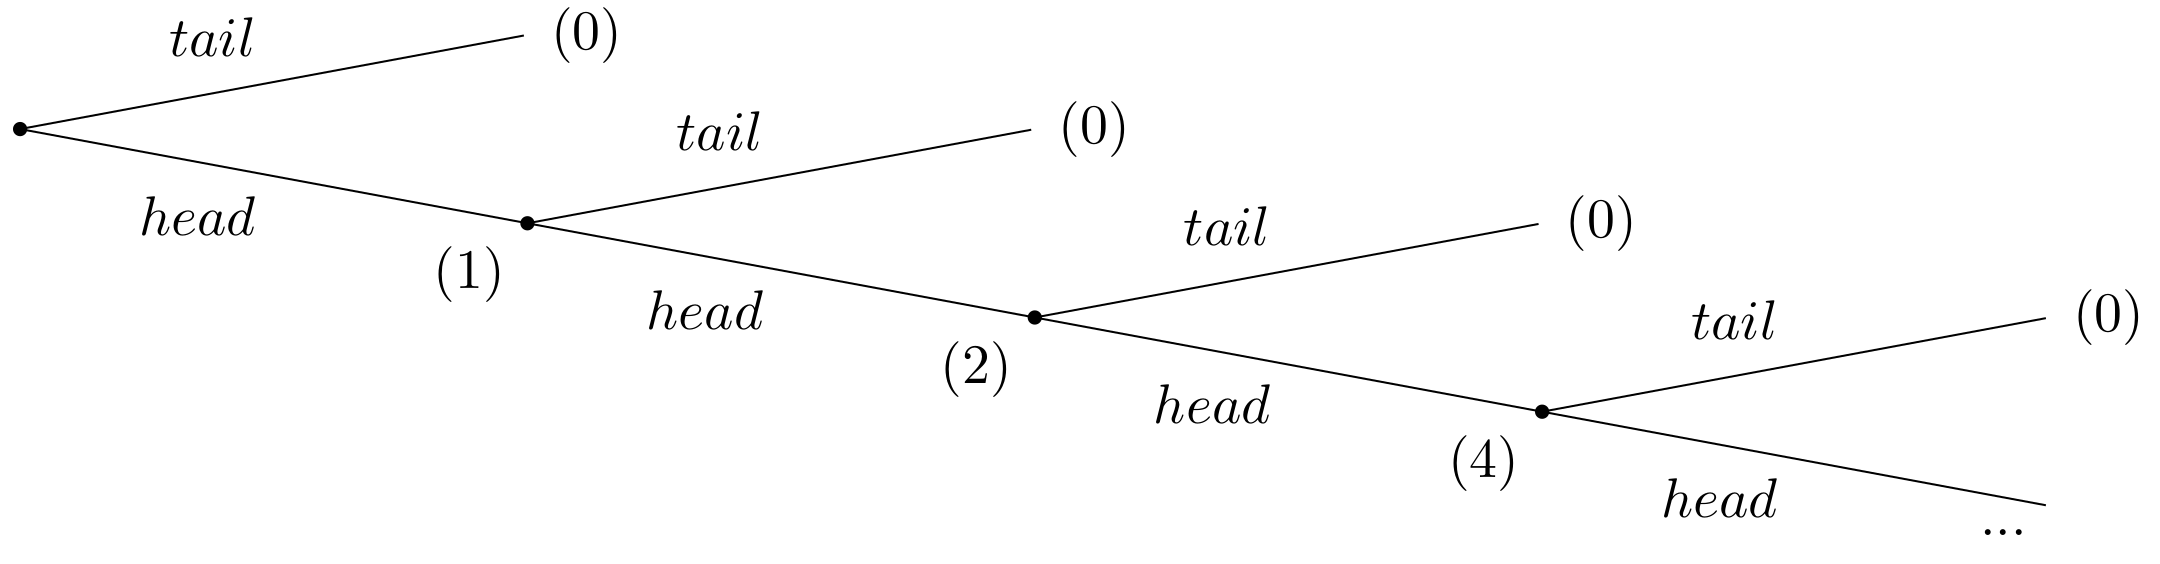
\includegraphics[width=0.8\textwidth,height=\textheight]{fig/spextensiveform.png}
\caption{\label{fig:spextensiveform} Extensive form of the St.~Petersburg paradox}
\end{figure}

The extensive form is given in figure \ref{fig:spextensiveform}.
First, the expected value of the game must now be calculated. For this the probability \(p(i)\) of throwing any number \(i\) of consecutive heads is crucial. This probability is given by
\[
p(i)=\underbrace{\frac{1}{2} \cdot \frac{1}{2} \cdot \cdots \frac{1}{2}}_{i \text { Faktoren }}=\frac{1}{2^{i}}
\]
The payoff \(W(i)\) is, if head appears \(i\)-times in a row by
\[
W(i)=2^{i-1}
\]
The expected payoff \(E(W(I))\) if the coin is flipped \(I\) times is then given by
\[
E(W(I))=\sum_{i=1}^{I} p(i) \cdot W(i)=\sum_{i=1}^{I} \frac{1}{2^{i}} \cdot 2^{i-1}=\sum_{i=1}^{I} \frac{1}{2}=\frac{I}{2}
\]

Thus, the expected payoff grows proportionally with the maximum number of rolls. This is because at any point in the game, the option to keep playing has a positive value no matter how many times head has appeared before.
Thus, the expected value of the game is infinitely high for an unlimited number of rolls. Even with a very limited maximum number of rolls of, for example, \(I = 100\), only a few players would be willing to pay
50 Euro for participation. The relatively high probability to leave the game with no or very low winnings leads in general to a subjective rather low evaluation that is below the expected value.

The basic idea of \emph{Daniel Bernoulli}, which enables a solution of this paradox lies in the conceptual separation of the expected payoff and its utility. He describes the basis of the paradox as follows:

\begin{quote}
``Until now scientists have usually rested their hypothesis on the assumption that all gains must be evaluated exclusively in terms of themselves, i.e., on the basis of their intrinsic qualities, and that these gains will always produce a utility directly proportionate to the gain.'\,' \citep[p.~27]{Bernoulli1954Exposition}
\end{quote}

Thus, we should evaluate the game in categories of expected utility:
\[
E(u(W(I)))=\sum_{i=1}^{I} p(i) \cdot u(W(i))=\sum_{i=1}^{I} \frac{1}{2^{i}} \cdot u\left(2^{i-1}\right)
\]
Daniel Bernoulli himself proposed the following logarithmic utility function:
\[
u(W)=a \cdot \ln (W),
\]
where \(a\) is a positive constant. Using this function in the expected utility, we get
\[
E(u(W(I)))=\sum_{i=1}^{I} \frac{1}{2^{i}} \cdot a \cdot \ln \left(2^{i-1}\right)=a \cdot \sum_{i=1}^{I} \frac{i-1}{2^{i}} \ln 2=a \cdot \ln 2 \cdot \sum_{i=1}^{I} \frac{i-1}{2^{i}}.
\]
The infinite series, \(\sum_{i=1}^{I} \frac{i-1}{2^{i}}\), converges to 1 (\(\lim _{I \rightarrow \infty} \sum_{i=1}^{I} \frac{i-1}{2^{i}}=1\)). Thus, given an ex ante unbounded number of throws, the expected utility of the game is given by
\[
E(u(W(\infty)))=a \cdot \ln 2 .
\]

In experiments in which people were offered this game, their willingness to pay was roughly between 2 and 3 Euro. Thus, the suggests logarithmic utility function seems to be a pretty realistic specification.
The main reason is mathematically that the increasing expected payoff has decreasing marginal utility and hence the utility function reflects the risk aversion of many people.

\begin{exercise}
\protect\hypertarget{exr:ratrisk}{}\label{exr:ratrisk}

Rationality and risk

There are 90 balls in an box. It is known that 30 of them are red, the remaining 60 are blue or green. An individual can choose between the following lotteries:

\begin{longtable}[]{@{}
  >{\centering\arraybackslash}p{(\columnwidth - 4\tabcolsep) * \real{0.3333}}
  >{\centering\arraybackslash}p{(\columnwidth - 4\tabcolsep) * \real{0.3333}}
  >{\centering\arraybackslash}p{(\columnwidth - 4\tabcolsep) * \real{0.3333}}@{}}
\toprule()
\begin{minipage}[b]{\linewidth}\centering
\end{minipage} & \begin{minipage}[b]{\linewidth}\centering
Payoff
\end{minipage} & \begin{minipage}[b]{\linewidth}\centering
probability
\end{minipage} \\
\midrule()
\endhead
Lottery 1 & 100 Euro if a red ball is drawn 0 Euro else & \(p=\frac{1}{3}\) \\
Lottery 2 & 100 Euro if a blue ball is drawn 0 Euro else & \(0 \leq p \leq \frac{2}{3}\) \\
\bottomrule()
\end{longtable}

In a second variant it has the choice between the following lotteries:

\begin{longtable}[]{@{}
  >{\raggedright\arraybackslash}p{(\columnwidth - 4\tabcolsep) * \real{0.3333}}
  >{\raggedright\arraybackslash}p{(\columnwidth - 4\tabcolsep) * \real{0.3333}}
  >{\raggedright\arraybackslash}p{(\columnwidth - 4\tabcolsep) * \real{0.3333}}@{}}
\toprule()
\begin{minipage}[b]{\linewidth}\raggedright
\end{minipage} & \begin{minipage}[b]{\linewidth}\raggedright
Payoff
\end{minipage} & \begin{minipage}[b]{\linewidth}\raggedright
probability
\end{minipage} \\
\midrule()
\endhead
Lottery 3 & 100 Euro if a red or green ball is drawn or 0 Euro else & \(\frac{1}{3} \leq p \leq 1\) \\
Lottery 4 & 100 Euro if a blue or green ball is drawn or 0 Euro else & \(p=\frac{2}{3}\) \\
\bottomrule()
\end{longtable}

\begin{enumerate}
\def\labelenumi{\alph{enumi})}
\tightlist
\item
  Which of the lotteries does the individual choose on the basis of expected values (risk neutral)?
\item
  Which of the lotteries does the individual choose on the basis of expected utility if the utility of a payoff of \(x\) is given by \(u(x) = x^2\)?
\item
  Empirical studies, e.g.~\cite{Camerer1992Recent}, show, however, that most individuals will usually choose lotteries 1 and 4. will. Discuss: Is this consistent with rational behavior?
\end{enumerate}

\end{exercise}

\hypertarget{decision-making-with-conditional-probabilities-bayes-theorem}{%
\section{Decision making with conditional probabilities (Bayes' theorem)}\label{decision-making-with-conditional-probabilities-bayes-theorem}}

\begin{center}\rule{0.5\linewidth}{0.5pt}\end{center}

After successful completion of the module, students are able to:

\begin{itemize}
\tightlist
\item
  Understand and use the terminology of probability.
\item
  Determine whether two events are mutually exclusive and whether two events are independent.
\item
  Calculate probabilities using the addition rules and multiplication rules.
\item
  Calculate with conditional probabilities using Bayes Theorem.
\item
  Construct and interpret venn and tree diagrams.
\item
  Apply their knowledge of probability theory to decision making in business.
\end{itemize}

\begin{center}\rule{0.5\linewidth}{0.5pt}\end{center}

\begin{figure}
\centering
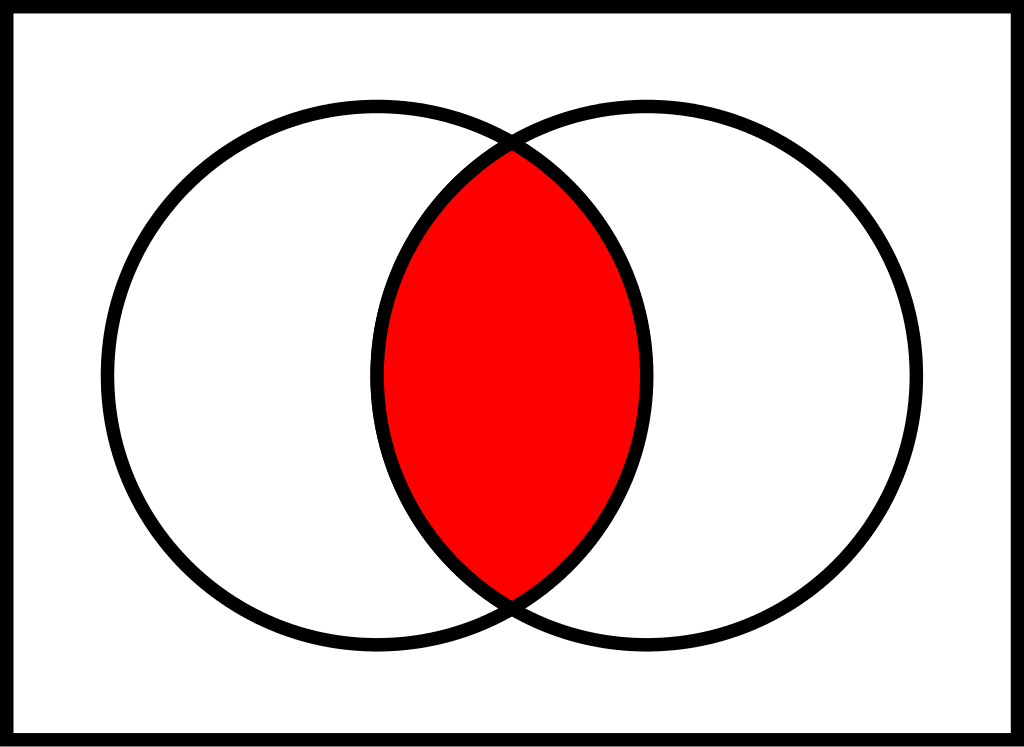
\includegraphics[width=0.3\textwidth,height=\textheight]{fig/intersection.png}
\caption{\label{fig:afig} Intersection: \(A \cap B\)}
\end{figure}

\begin{figure}
\centering
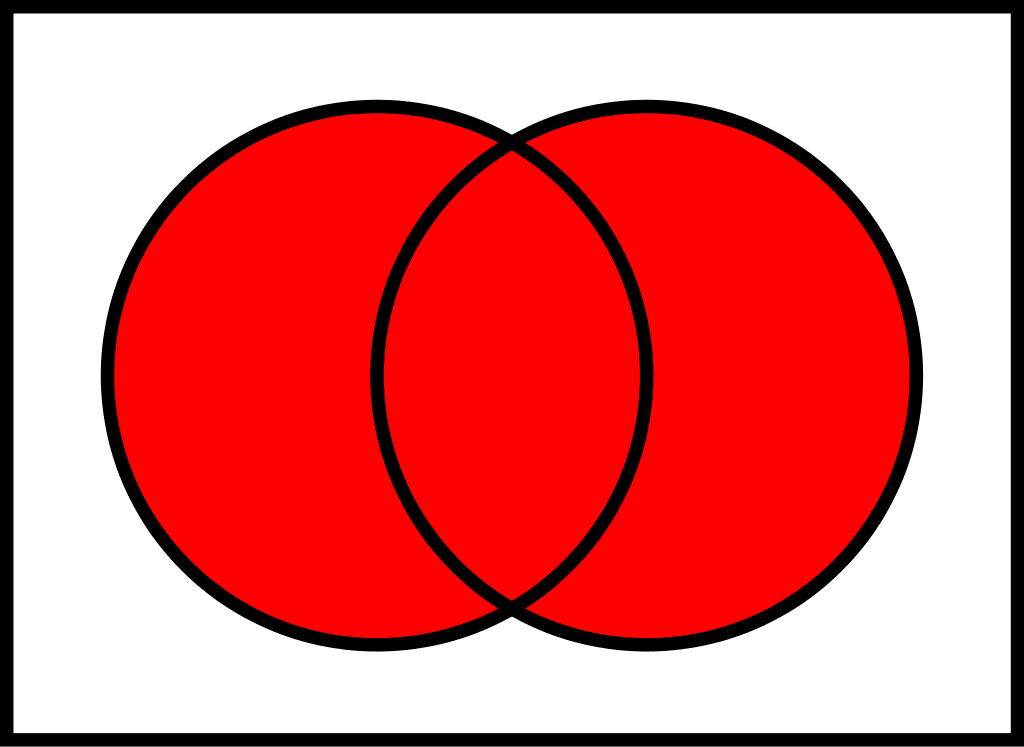
\includegraphics[width=0.3\textwidth,height=\textheight]{fig/union.png}
\caption{\label{fig:bfig} Union: \(A \cup B\)}
\end{figure}

\begin{figure}
\centering
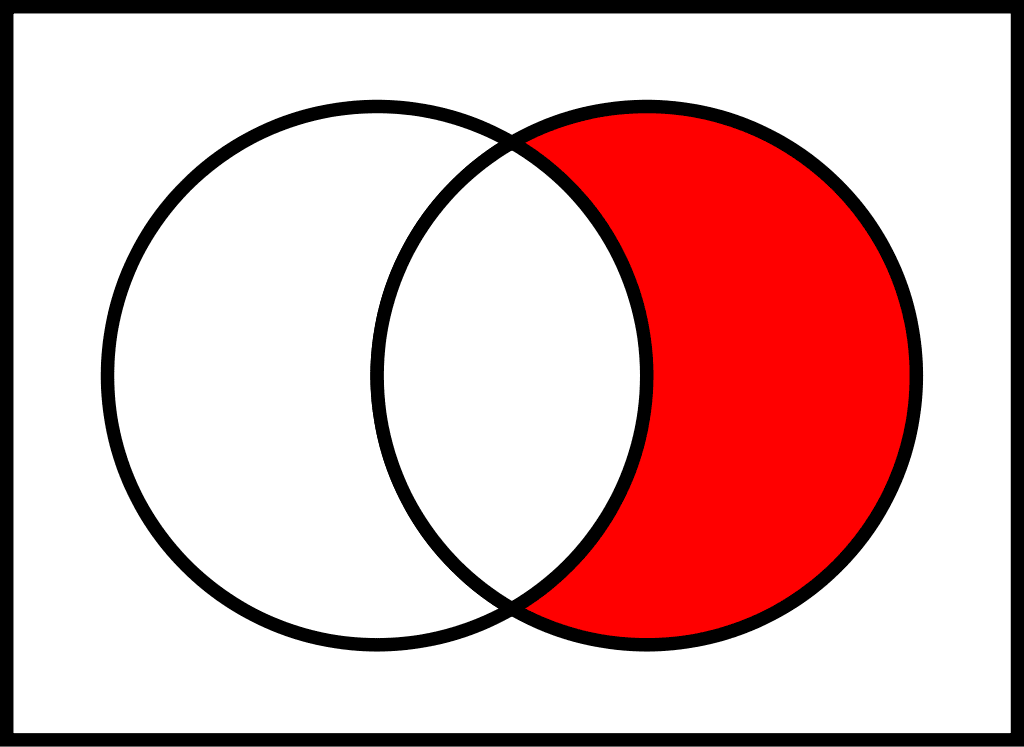
\includegraphics[width=0.3\textwidth,height=\textheight]{fig/notA.png}
\caption{\label{fig:cfig} Relative complement: \(\neg A \cup B\)}
\end{figure}

\hypertarget{school-stuff}{%
\subsubsection*{School Stuff}\label{school-stuff}}

The next chapter will deal with stochastics. In Germany, stochastics is taught in the Gymnasium. If you are not from Germany, it was probably also part of your school experience. When I moved to Cologne in 2020, I found the following page shown in figure \ref{fig:inschool} that I had received from my high school math teacher. It was September 1993 and I was a desperate fifth grader in my fourth week. Perhaps you'd like to share your experiences with stochastics?

\begin{figure}
\centering
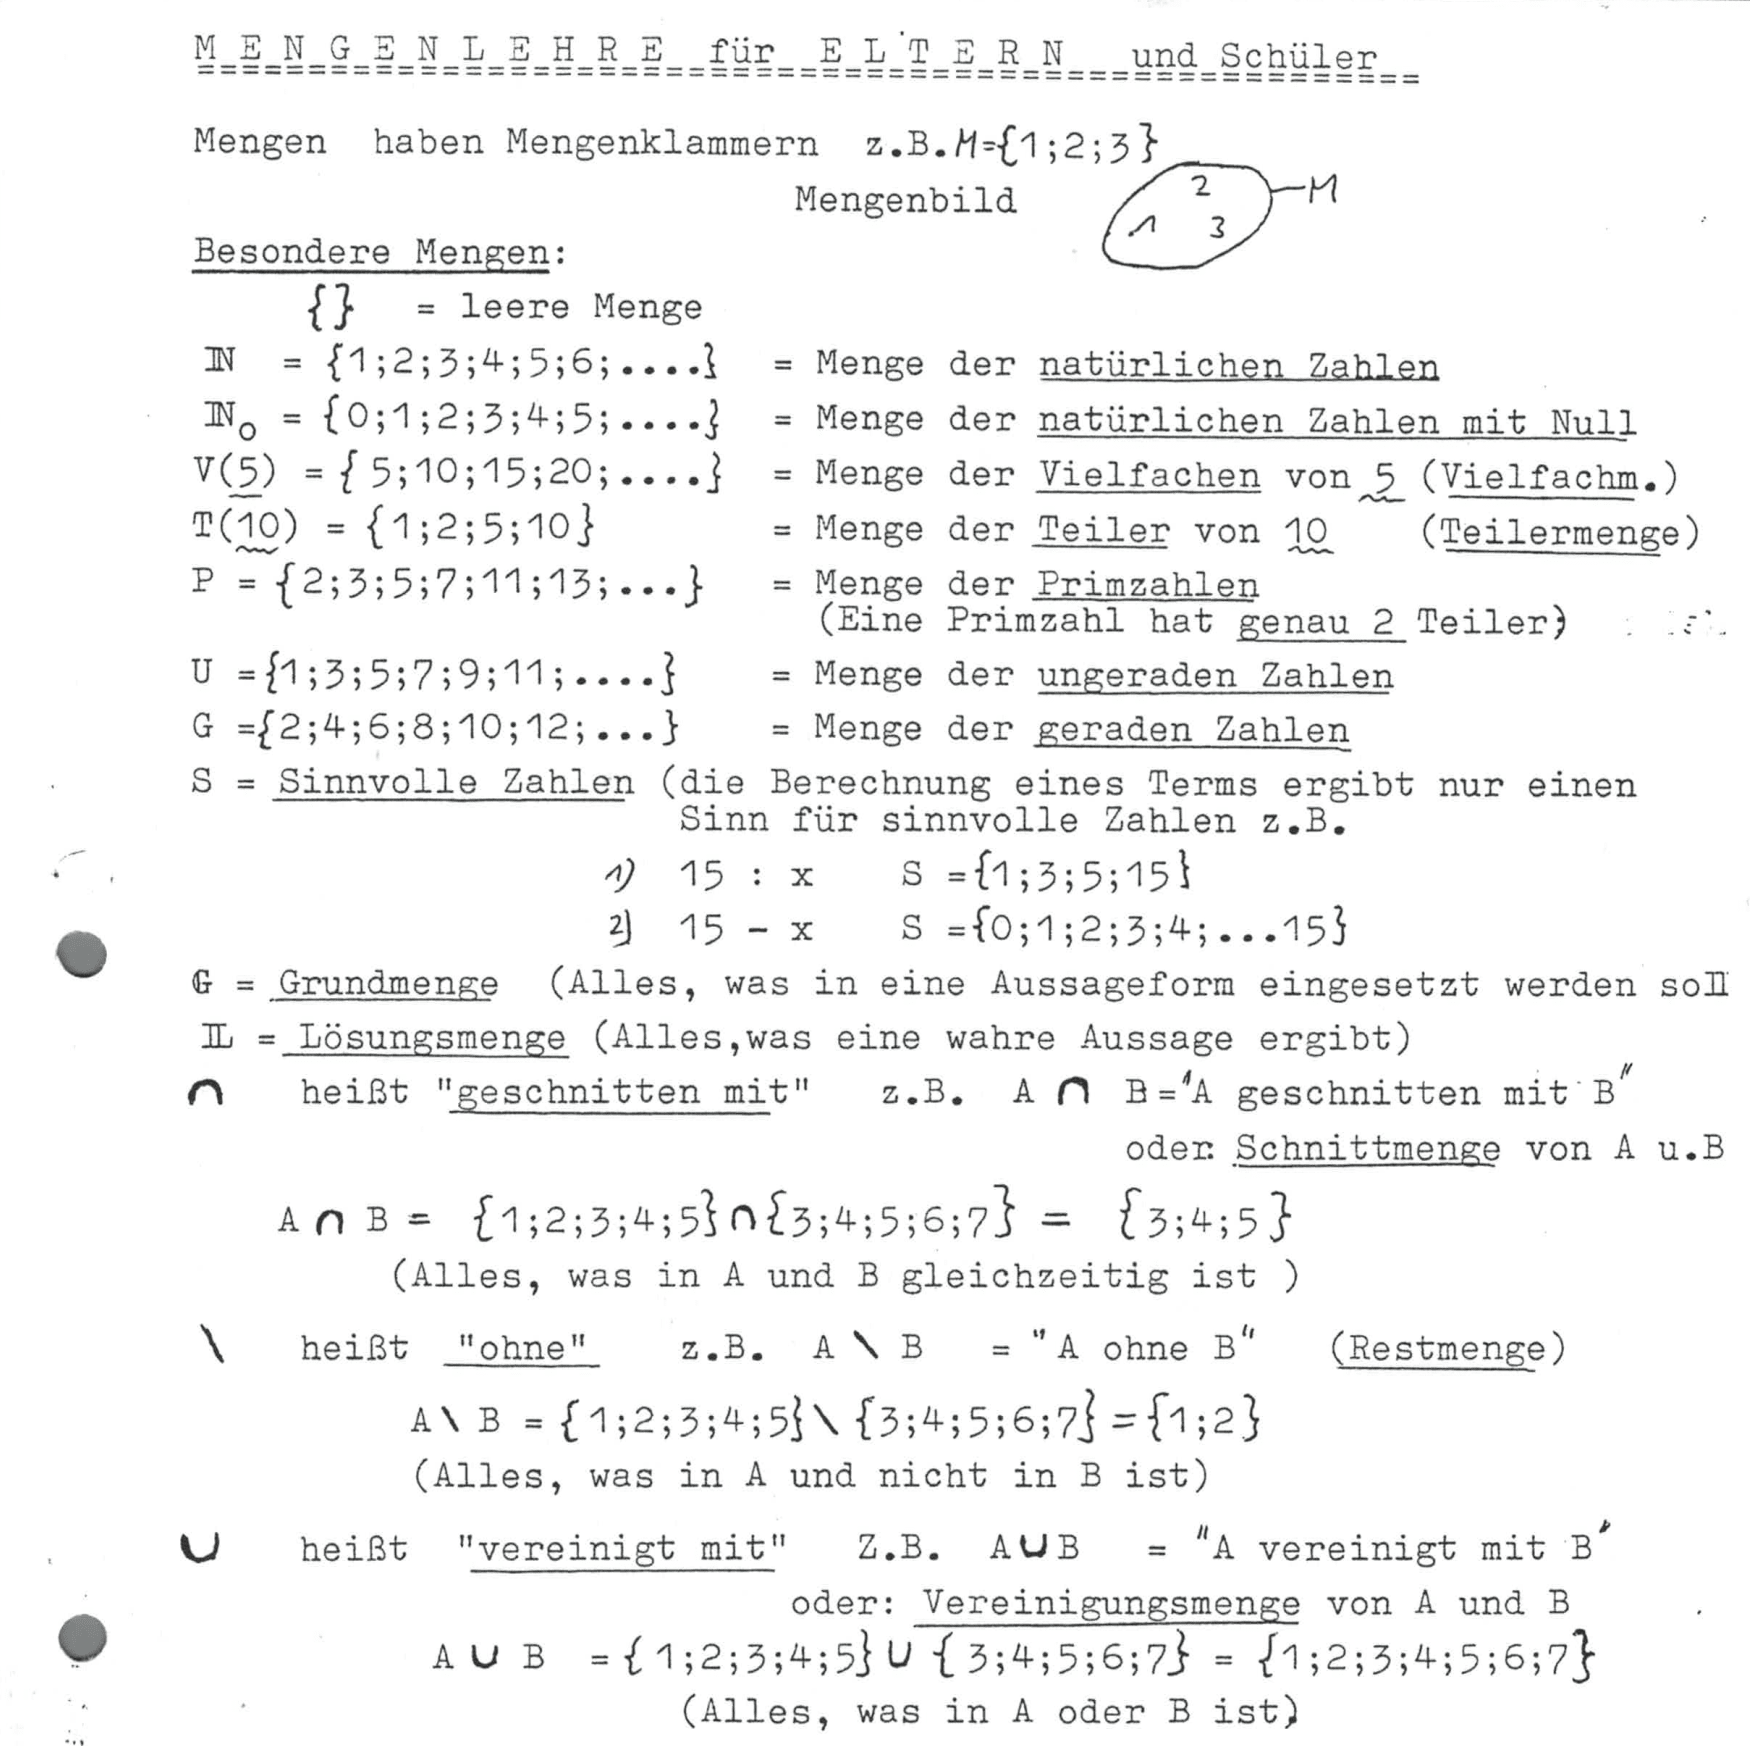
\includegraphics[width=0.9\textwidth,height=\textheight]{fig/mengenlehre-5.png}
\caption{\label{fig:inschool} Relative complement: \(\neg A \cup B\)}
\end{figure}

\hypertarget{terminology-pa-pab-omega-cap-neg}{%
\subsection{\texorpdfstring{Terminology: \(P(A)\), \(P(A|B)\), \(\Omega\), \(\cap\), \(\neg\), \ldots{}}{Terminology: P(A), P(A\textbar B), \textbackslash Omega, \textbackslash cap, \textbackslash neg, \ldots{}}}\label{terminology-pa-pab-omega-cap-neg}}

\hypertarget{sample-space}{%
\subsubsection{Sample space}\label{sample-space}}

A result of an \emph{experiment} is called an \emph{outcome}. An experiment is a planned operation carried out under controlled conditions. Flipping a fair coin twice is an example of an experiment.
The \emph{sample space} of an experiment is the set of all possible outcomes.
The Greek letter \(\Omega\) is often used to denote the sample space. For example, if you flip a fair coin, \(\Omega = \{H, T\}\) where the outcomes heads and tails are denoted with \(H\) and \(T\), respectively.

\textbf{Example: Sample space}
Find the sample space for the following experiments:

\begin{enumerate}
\def\labelenumi{\alph{enumi})}
\tightlist
\item
  One coin is tossed.
\item
  Two coins are tossed once.
\item
  Two dices are tossed once.
\item
  Picking two marbles, one at a time, from a bag that contains many blue, \(B\), and red marbles, \(R\).
\end{enumerate}

\textbf{Solutions:}

\begin{enumerate}
\def\labelenumi{\alph{enumi})}
\tightlist
\item
  \(\Omega = \{head, tail\}\)
\item
  \(\Omega = \{(head, head), (tail, tail),(head, tail),(tail, head)\}\)
\item
  Overall, 36 different outcomes:
  \(\{  (1,1),(1,2),(1,3),(1,4),(1,5),(1,6),(2,1),(2,2),\dots,(6,6)  \}\)
\item
  \(\Omega = \{(B,B), (B,R), (R,B), (R,R)\}\).
\end{enumerate}

Overall, there are three ways to represent a sample space:

\begin{enumerate}
\def\labelenumi{\arabic{enumi}.}
\tightlist
\item
  to list the possible outcomes (see example above),
\item
  to create a tree diagram (see \ref{fig:decisiontree}), or
\item
  to create a Venn diagram (see \ref{fig:venndiagramm}).
\end{enumerate}

\begin{figure}
\centering
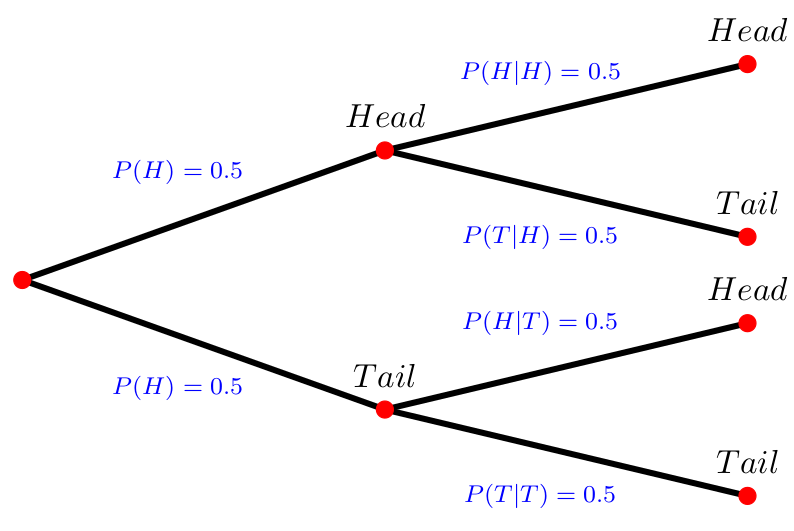
\includegraphics[width=0.5\textwidth,height=\textheight]{fig/treedia.png}
\caption{\label{fig:decisiontree} Tree diagramm}
\end{figure}

\begin{figure}
\centering
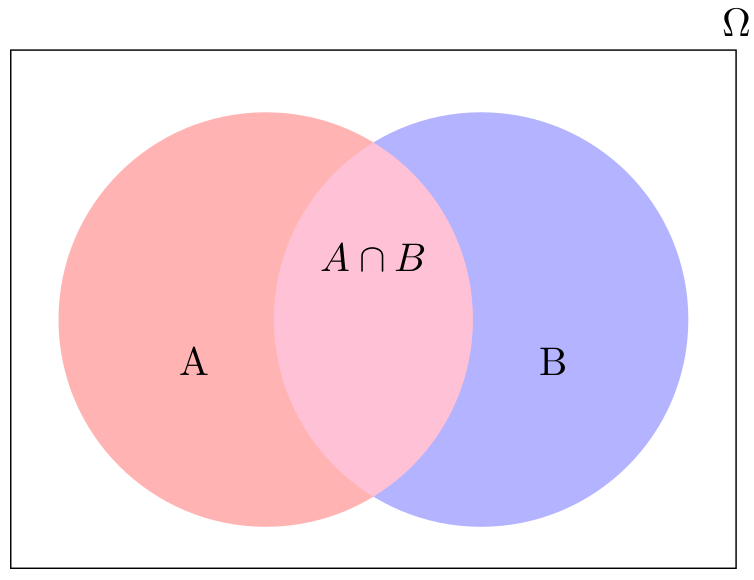
\includegraphics[width=0.25\textwidth,height=\textheight]{fig/venndia.png}
\caption{\label{fig:venndiagramm} Venn diagramm}
\end{figure}

\hypertarget{probability}{%
\subsubsection{Probability}\label{probability}}

Probability is a measure that is associated with how certain we are of outcomes of a particular experiment or activity. The probability of an event \(A\), written \(P(A)\), is defined as
\[
P(A)=\frac{\
text{Number of outcomes favorable to the occurrence of } A}{\text{Total number of equally likely outcomes}}=\frac{n(A)}{n(\Omega)}
\]
For example, A dice has 6 sides with 6 different numbers on it. In particular, the set of \emph{elements} of a dice is \(M=\{1,2,3,4,5,6\}\). Thus, the probability to receive a 6 is 1/6 because we look for one wanted outcome in six possible outcomes.

\textbf{Example: Probability}

When a fair dice is thrown, what is the probability of getting

\begin{enumerate}
\def\labelenumi{\alph{enumi})}
\tightlist
\item
  the number 5,
\item
  a number that is a multiple of 3,
\item
  a number that is greater than 6,
\item
  a positive number that is less than 7.
\end{enumerate}

\textbf{Solutions:} A fair dice is an unbiased dice where each of the six numbers is equally likely to turn up. The sample space is \(\Omega = \{1, 2, 3, 4, 5, 6\}\).

\begin{enumerate}
\def\labelenumi{\alph{enumi})}
\tightlist
\item
  Let A be the event of getting the number 5, \(A=\{5\}\). Then, \(P(A)=\frac{1}{6}\).
\item
  Let \(B\) be the event of getting a multiple of 3, \(B=\{3, 6\}\). Then, \(P(B)=\frac{1}{3}\).
\item
  Let \(C\) be the event of getting a number greater than 6, \(C=7,8,\dots\). Then, \(P(C)=0\) as there is no number greater than 6 in the sample space \(\Omega=\{1,2,3,4,5,6\}\). A probability of 0 means the event will never occur.
\item
  Let D be the event of getting a number less than 7, \(D=\{1,2,3,4,5,6\}\). Then, \(P=1\) as the event will always occur.
\end{enumerate}

\hypertarget{the-complement-of-an-event-neg-event}{%
\subsubsection{\texorpdfstring{The complement of an event (\(\neg-Event\))}{The complement of an event (\textbackslash neg-Event)}}\label{the-complement-of-an-event-neg-event}}

The complement of event \(A\) is denoted with a \(\neg A\) or sometimes with a superscript `c' like \(A^c\).
It consists of all outcomes that are \emph{not} in \(A\). Thus, it should be clear that \(P(A) + P(\neg A) =! 1\).
For example, let the sample space be \(\Omega = \{1, 2, 3, 4, 5, 6\}\) and let \(A = \{1, 2, 3, 4\}\).
Then, \(\neg A = \{5, 6\}\); \(P(A) = \frac{4}{6}\); \(P(\neg A) = \frac{2}{6}\); and \(P(A) + P(\neg A) = \frac{4}{6}+\frac{2}{6} = 1\).

\hypertarget{independent-events-and-events}{%
\subsubsection{Independent events (AND-events)}\label{independent-events-and-events}}

Two events are independent when the outcome of the first event does not influence the outcome of the second event.
For example, if you throw a dice and a coin, the number on the dice does not affect whether the result you get on the coin.
More formally, two events are independent if the following are true:
\begin{align*}
    P(A|B) &= P(A)\\
    P(B|A) &= P(B)\\
    P(A \cap B) &= P(A)P(B)
\end{align*}

To calculate the probability of two independent events (\(X\) and \(Y\)) happen, the probability of the first event, \(P(X)\), has to be multiplied with the probability of the second event, \(P(Y)\):
\[ P(X \text{ and } Y)=P(X \cap Y)=P(X)\cdot P(Y),\]
where \(\cap\) stands for `and'.
For example, let \(A\) and \(B\) be \(\{1, 2, 3, 4, 5\}\) and \(\{4, 5, 6, 7, 8\}\), respectively. Then \(A \cap B = \{4, 5\}\).

\textbf{Example: Three dices}

Suppose you have three dice. Calculate the probability of getting three 4\$.\}

\textbf{Solutions:}
The probability of getting a \(4\) on one dice is 1/6. The probability of getting three \(4\) is:
\[
P(4 \cap 4 \cap 4) = \frac{1}{6}\cdot \frac{1}{6}\cdot \frac{1}{6}= \frac{1}{216}
\]

\hypertarget{dependent-events--events}{%
\subsubsection{\texorpdfstring{Dependent events (\(|\)-Events)}{Dependent events (\textbar-Events)}}\label{dependent-events--events}}

Events are dependent when one event affects the outcome of the other. If \(A\) and \(B\) are dependent events then the probability of both occurring is the product of the probability of \(A\) and the probability of \(A\) \emph{after} \(B\) has occurred:
\begin{align*}
    P(A \cap B)&=P(A)\cdot P(B|A),\\
    \Leftrightarrow P(B|A)&=\frac{P(A \cap B)}{P(A)}\cdot 
\end{align*}
where \texttt{\$\textbar{}A\$\textquotesingle{}\ stands\ for}after A has occurred', or `given A has occurred'. In other words, \(P(B|A)\) is the probability of \(B\) given \(A\). This equation is also known as the \textbf{Multiplication Rule}.

The conditional probability of A given B is written \(P(A|B)\). \(P(A|B)\) is the probability that event A will occur given that the event B has already occurred. A conditional reduces the sample space. We calculate the probability of A from the reduced sample space B. The formula to calculate \(P(A|B)\) is \[ P(A|B) = \frac{P\left(A\cap B\right)}{P\left(B\right)}\] where \(P(B)\) is greater than zero.
This formula is also known as \textbf{Bayes' Theorem}, which is a simple mathematical formula used for calculating conditional probabilities, states that
\[
P(A)P(B|A)=P(B)P(A|B)
\]
This is true since \(P(A \cap B)=P(B \cap A)\) and due to the fact that \(P(A\cap B)=P(B\mid A)P(A)\), we can write Bayes' Theorem as
\[P(A\mid B)={\frac {P(B\mid A)P(A)}{P(B)}}.\]
The box below summarizes the important facts w.r.t. Bayes' Theorem.

For example, suppose we toss a fair, six-sided die. The sample space \(\Omega = \{1, 2, 3, 4, 5, 6\}\). Let \(A\) be face is 2 or 3 and let \(B\) be face is even (2, 4, 6). To calculate \(P(A|B)\), we count the number of outcomes 2 or 3 in the sample space \(B = \{2, 4, 6\}\). Then we divide that by the number of outcomes \(B\) (rather than \(\Omega\)).

We get the same result by using the formula. Remember that \(\Omega\) has six outcomes.
\[P(A\mid B)=\frac{P(B\cap A)}{P(B)} = \frac{\frac{\text{number of outcomes that are 2 or 3 and even}}{6}}{\frac{\text{number of outcomes that are even}}{6}}=\frac{\frac{1}{6}}{\frac{3}{6}}=\frac{1}{3} \]

\hypertarget{bayes-theorem}{%
\subsection{Bayes' Theorem}\label{bayes-theorem}}

The theorem states that
\[P(A\mid B)={\frac {P(B\mid A)P(A)}{P(B)}} \]
if \(P(B)\neq 0\) and \(A\) and \(B\) are events. It simply uses the following logical facts:
\[P(B\cap A)=P(A\cap B),\]
\[P(A\mid B)=\frac {P(A\cap B)}{P(B)},  \text{ and}\]
\[P(B\mid A)=\frac {P(A\cap B)}{P(A)},\]
or, to put it in one line:
\[  P(A\cap B)= P(B\cap A)=P(A\mid B)P(B)=P(B\mid A)P(A).   \]
Sometimes, it is helpful to re-write the Theorem as follows:
\[P(A)=P(A|B)P(B)+P(A|\neg B)P(\neg B),  \text{ and}\]
\[P(B)=P(B|A)P(A)+P(B|\neg A)P(\neg A),\]

\textbf{Example: Purse}

A purse contains four € 5 bills, five € 10 bills and three € 20 bills. Two bills are selected randomly without the first selection being replaced. Find the probability that two € 5 bills are selected.

\textbf{Solutions:} There are four € 5 bills. There are a total of twelve bills.
The probability to select at first a € 5 bill then is \(P(€ 5) = \frac{4}{12}\).
As the the result of the first draw affects the probability of the second draw, we have to consider that there are only three € 5 bills left and there are a total of eleven bills left. Thus,
\[
P(€ 5 | € 5)=\frac{3}{11}
\]
and
\[
P(€ 5 \cap € 5) = P(€ 5) \cdot P(€ 5 | € 5) = \frac{4}{12} \cdot \frac{3}{11}=\frac{1}{11}.
\]
The probability of drawing a € 5 bill and then another € 5 bill is \(\frac{1}{11}\).

Watch the videos\\
\href{https://youtu.be/HZGCoVF3YvM}{Bayes theorem} and
\href{https://youtu.be/U_85TaXbeIo}{The quick proof of Bayes' theorem}

Moreover, consider this interactive tool: \url{https://www.skobelevs.ie/BayesTheorem/}

\begin{exercise}
\protect\hypertarget{exr:tobevacornot}{}\label{exr:tobevacornot}

To be vaccinated or not to be

\begin{figure}
\centering
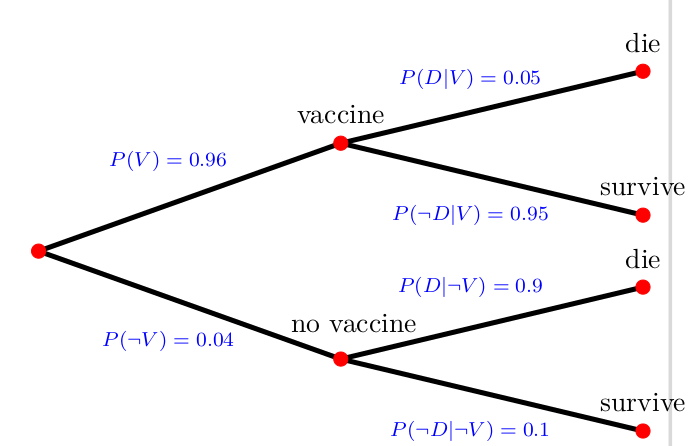
\includegraphics[width=0.5\textwidth,height=\textheight]{fig/diesurvive.png}
\caption{\label{fig:diesurvive} Tree diagramm vaccinated or not}
\end{figure}

The \emph{Tree Diagram} in figure \ref{fig:diesurvive} shows probabililties of people to have a vaccine for some disease. Moreover, it shows the conditional probabilities of people to die given the fact they were vaccinated or not.
\(D\) denotes the event of \emph{die} and \(\neg D\) denotes \emph{not die}, i.e., survive; \(V\) denotes the event of \emph{vaccinated} and \(\neg V\) \emph{not vaccinated}.

\begin{enumerate}
\def\labelenumi{\alph{enumi})}
\tightlist
\item
  Calculate the overall probability to die, \(P(D)\)
\item
  Calculate the probability that a person that has died was vaccinated, \(P(V|D)\).
\end{enumerate}

Please find solution to the exercise \protect\hyperlink{sol:tobevacornot}{in the appendix.}

\begin{quote}
Disclaimer: The case presented here is fictitious. The data given here are purely fictitious and serve only to practice the method.
\end{quote}

\end{exercise}

\begin{exercise}
\protect\hypertarget{exr:todieornot}{}\label{exr:todieornot}To die or not to die

You read on Facebook that in the year 2021 about over 80\% of people that died were vaccinated. You are shocked by this high probability that a dead person was vaccinated, \(P(V|D)\). You decide to check this fact. Reading the study to which the Facebook post is referring, you find out that the study only refers to people above the age of 90. Moreover, you find the following \emph{Tree Diargram}. It allows checking the fact as it describes the vaccination rates and the conditional probabilities of people to die given the fact they were vaccinated or not.
In particular, \(D\) denotes the event of \emph{die} and \(\neg D\) denotes \emph{not die}, i.e., survive; \(V\) denotes the event of \emph{vaccinated} and \(\neg V\) \emph{not vaccinated}.
\end{exercise}

\begin{figure}
\centering
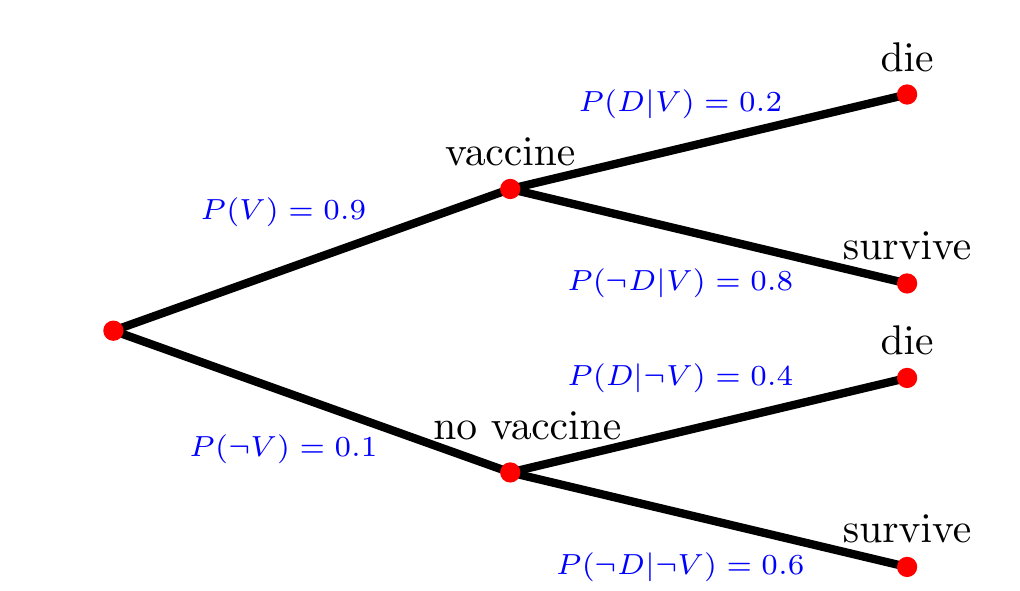
\includegraphics{_main_files/figure-latex/tikz-ex2-1.png}
\caption{\label{fig:tikz-ex2}Tree: To die or not to die}
\end{figure}

\begin{enumerate}
\def\labelenumi{\alph{enumi})}
\tightlist
\item
  Calculate the overall probability to die, \(P(D)\)
\item
  Calculate the probability that a person that has died was vaccinated, \(P(V|D)\).
\item
  Your calculations shows that the fact used in the statement on Facebook is indeed true. Discuss whether this number should have an impact to get vaccinated or not.
\end{enumerate}

\begin{quote}
Disclaimer: The case presented here is fictitious. The data given here are purely fictitious and serve only to practice the method.
\end{quote}

Please find solution to the exercise \protect\hyperlink{sol:todieornot}{in the appendix.}
```

\begin{exercise}
\protect\hypertarget{exr:falspos}{}\label{exr:falspos}Corona false positive

Suppose that Corona infects one out of every 1000 people in a population and that the test for it comes back positive in 99\% of all cases if a person has Corona. Moreover, the test also produces some false positive, that is about 2\% of uninfected patients also tested positive.

Now, assume you are tested positive and you want to know the chances of having the disease.
Then, we have two events to work with:

\textbf{A}: you have Corona

\textbf{B}: your test indicates that you have Corona

and we know that
\begin{align*}
    P(A)&=.001  \qquad \rightarrow \text{one out of 1000 has Corona}\\
    P(B|A)&=.99 \qquad \rightarrow \text{probability of a positive test, given infection}\\
    P(B|\neg A)&=.02 \qquad \rightarrow \text{probability of a false positive, given no infection}
\end{align*}

As you don`t like to go into quarantine, you are interested in the probability of having the disease given a positive test, that is \(P(A|B)\)?

\begin{quote}
Disclaimer: The case presented here is fictitious. The data given here are purely fictitious and serve only to practice the method.
\end{quote}

Please find solution to the exercise \protect\hyperlink{sol:falspos}{in the appendix.}
\end{exercise}

\hypertarget{appendix}{%
\chapter{Appendix}\label{appendix}}

\hypertarget{solutions-to-exercises}{%
\section{Solutions to exercises}\label{solutions-to-exercises}}

\hypertarget{sol:santa}{%
\subsection*{Solution to exercise \ref{exr:santa}: What is the house of Santa Claus?}\label{sol:santa}}

\begin{figure}
\centering
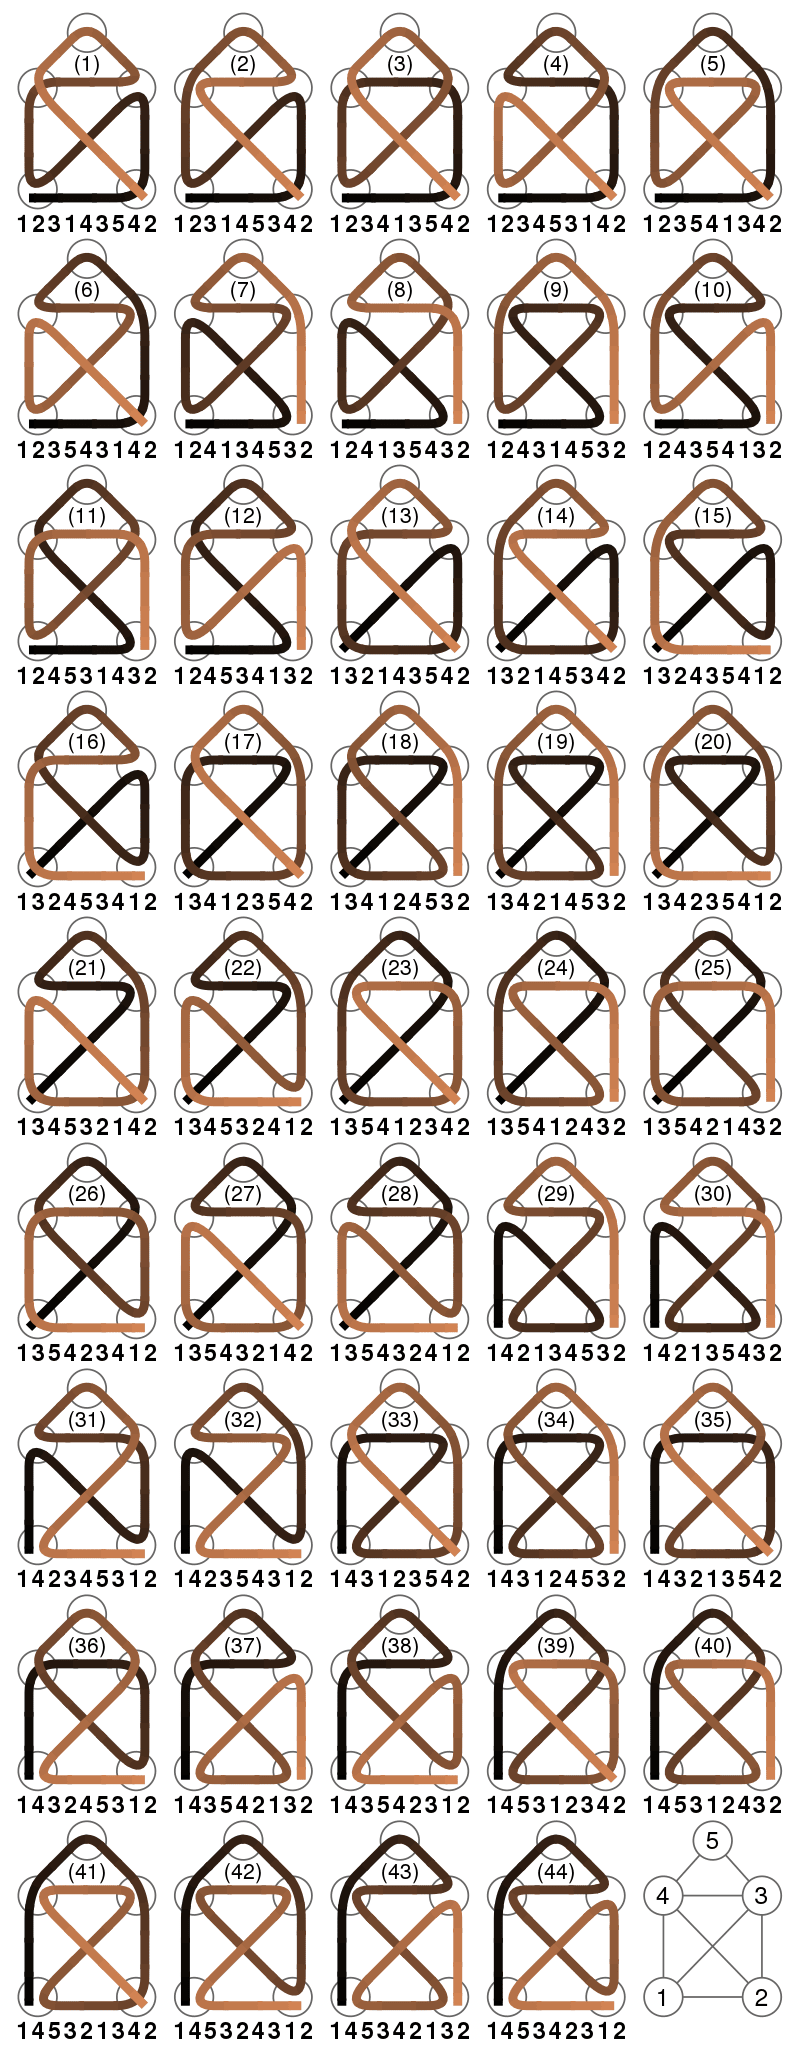
\includegraphics[width=0.5\textwidth,height=\textheight]{fig/nikolaus2.png}
\caption[\label{fig:nikolaus2} Forty-four ways to solve the puzzle]{\label{fig:nikolaus2} Forty-four ways to solve the puzzle\footnotemark{}}
\end{figure}
\footnotetext{Taken from \url{https://de.wikipedia.org/wiki/Haus_vom_Nikolaus}}

\begin{figure}
\centering
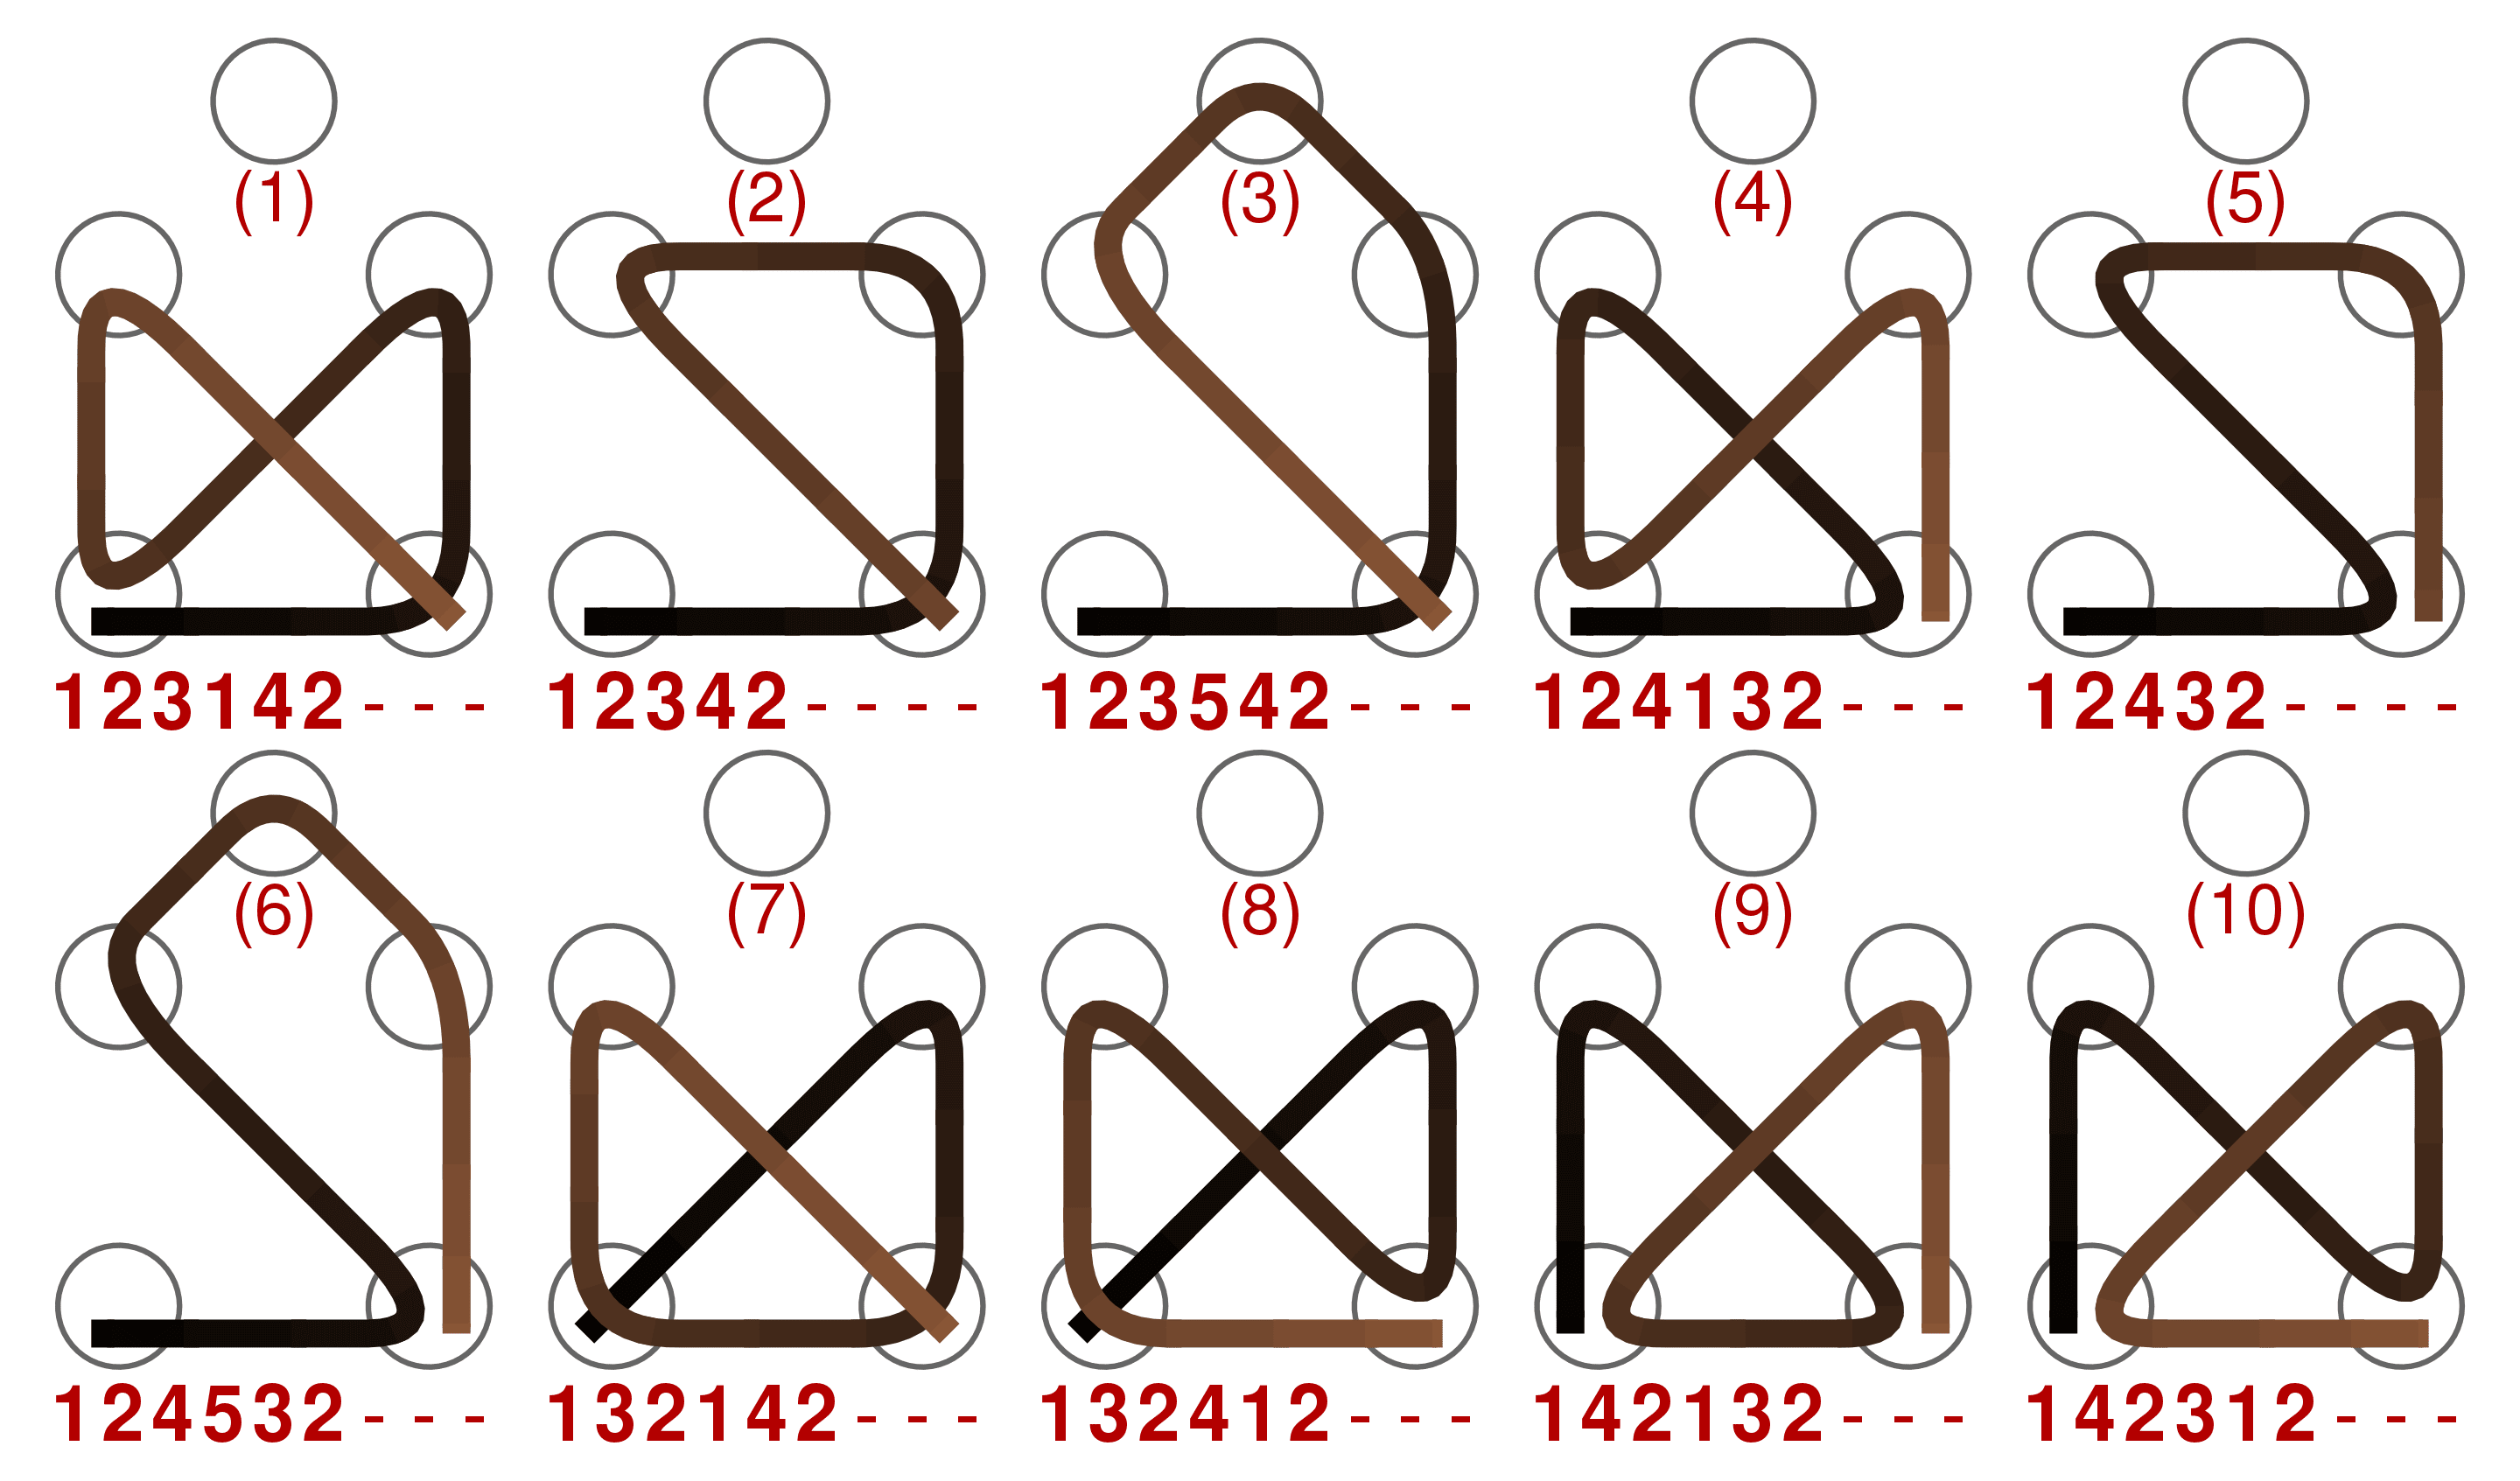
\includegraphics[width=0.5\textwidth,height=\textheight]{fig/nikolaus3.png}
\caption[\label{fig:nikolaus3} Ten ways to fail in the puzzle]{\label{fig:nikolaus3} Ten ways to fail in the puzzle\footnotemark{}}
\end{figure}
\footnotetext{Taken from \url{https://de.wikipedia.org/wiki/Haus_vom_Nikolaus}}

There are 44 solutions and only 10 different ways to fail. Thus, the probability to fail is about 18.5\% and hence the probability to succeed is about 81.5\%. In the course 10 persons participated in the poll. Here are the answers:

\begin{figure}
\centering
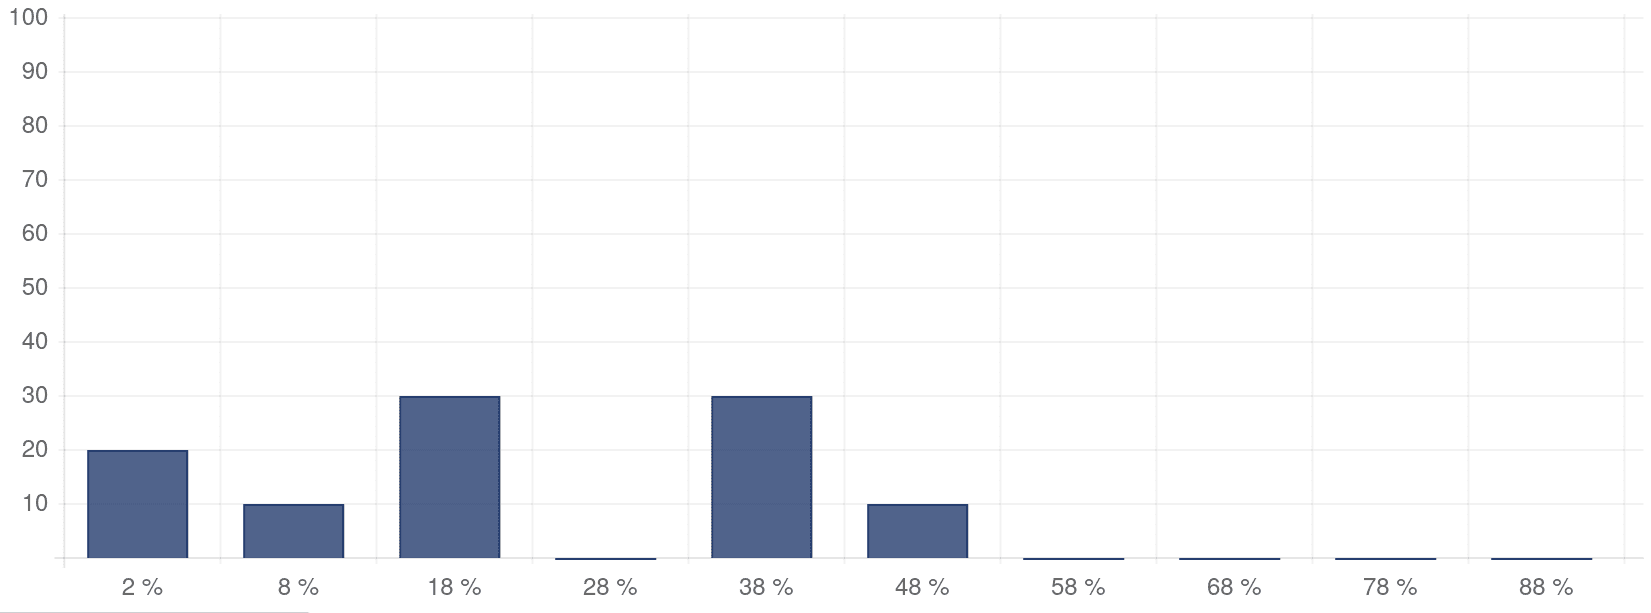
\includegraphics[width=0.75\textwidth,height=\textheight]{fig/nikolaus-poll.png}
\caption{\label{fig:nikolaus-poll} PINGO}
\end{figure}

Nobody came close to the correct probability.

\hypertarget{sol:opti-sati}{%
\subsection*{Solution to exercise \ref{exr:opti-sati}: Optimal vs.~satisfactory solution}\label{sol:opti-sati}}

\begin{enumerate}
\def\labelenumi{\Alph{enumi})}
\tightlist
\item
  Collecting and analyzing the available information about a product is costly. It is also difficult to analyze the importance of product features for the intended purpose.
\item
  Individuals often use rules of thumb to make a satisfactory decision.
\item
  It is difficult to understand complex situations such as the market for financial products. For some people, it is simply not possible to find the best product in these complex markets.
\item
  Consumers are often confronted with many variants of a product. The differences are negligible and therefore it is not worthwhile for consumers to analyze the situation in detail. Thus, they make a decision that may not be optimal, but they are satisfied with it.
\end{enumerate}

\hypertarget{sol:lisapregnant}{%
\subsection*{Solution to exercise \ref{exr:lisapregnant}: Lisa is pregnant}\label{sol:lisapregnant}}

At the beginning of the \emph{Inferential Statistics} course at summer 2020, I also asked student this question. Here are the results of the 16 students who participated:

\begin{longtable}[]{@{}lll@{}}
\toprule()
Option & Frequency of answers & Percentage \\
\midrule()
\endhead
a) & 3 & 19\% \\
b) & 2 & 13\% \\
c) & 2 & 13\% \\
d) & 3 & 19\% \\
e) & 6 & 38\% \\
\bottomrule()
\end{longtable}

How did they reach their answers? Like most people, they decided that Lisa has a substantial chance of having a baby with Down syndrome. The test gets it right 86 percent of the time, right? That sounds rather reliable, doesn't it? Well it does, but we should not rely on our feelings here and better do the math because the correct result would be that there is \textbf{just a 1.7 percent chance of the baby having a Down syndrome}.

Now, let us proof the result that there is just a 1.7 percent chance of the baby having a Down syndrome using \emph{Bayesian Arithmetic} which is explained in the following videos:

Also, consider this interactive tool here: \url{https://www.skobelevs.ie/BayesTheorem/}

Let \(A\) be the event of the Baby has a Down syndrom and \(B\) the test is positive. Then,
\begin{align*}
    P(A)&=0.001\\
    P(B\mid A)&=0.86\\
    P(B\mid \neg A)&=0.05\\
    P(B)&=\frac{999\cdot 0.05}{1000}+\frac{1\cdot 0.86}{1000}=\frac{50.81}{1000}=0.05081\\
    P(A\mid B)&={\frac {P(B\mid A)P(A)}{P(B)}}=\frac{0.86 \cdot 0.001}{0.05081}=0.016925802
\end{align*}

\hypertarget{sol:koerth-example}{%
\subsection*{Solution to exercise \ref{exr:koerth-example}: Körth: example}\label{sol:koerth-example}}

\(\overline{O}_1=5; \overline{O}_2=1; \overline{O}_3=7; \overline{O}_4=3; \overline{O}_5=4\)

\begin{longtable}[]{@{}lllllll@{}}
\toprule()
\(O_{ij}\) & \(k_1\) & \(k_2\) & \(k_3\) & \(k_4\) & \(k_5\) & \(\Phi(a_i)\) \\
\midrule()
\endhead
\(a_1\) & 3/5 & 0 & 1 & 1/3 & 1 & 0 \\
\(a_2\) & 4/5 & 0 & 4/7 & 2/3 & 1/4 & 0 \\
\(a_3\) & 4/5 & -1 & 3/7 & 2/3 & 1/4 & -1 \\
\(a_4\) & 1 & 1 & 3/7 & 1 & 1/4 & 1/4 \\
\bottomrule()
\end{longtable}

\(a_4\succ a_1 \sim a_2 \succ a_3\)

\hypertarget{sol:burger}{%
\subsection*{Solution to exercise \ref{exr:burger}: Burgers and drinks}\label{sol:burger}}

In the plot, I marked all 19 possible bundles of burger and drinks of consumption. The budget constraint is shown by the solid line.

\begin{figure}
\centering
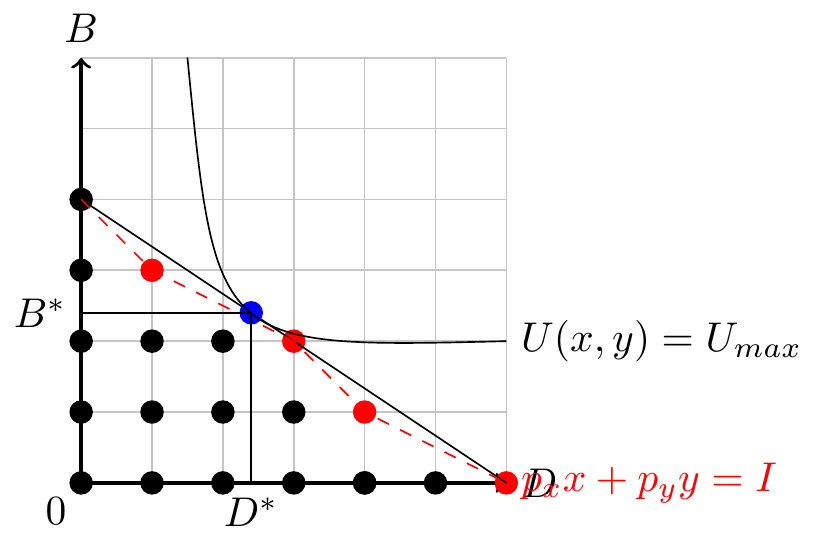
\includegraphics{_main_files/figure-latex/tikz-ex-1.png}
\caption{\label{fig:tikz-ex}Possible bundles of consumption}
\end{figure}

We now should calculate the utility of all 19 points but only the red dots denote choices that may yield an optimal utility. The best utility is at when we buy 2 burger and 3 drinks: \[U=2^{.6}3^{.4}=2.35\]

Solve:
\[
        \mathcal{L}=B^{0.6}D^{0.4}+\lambda(3B+2D-12)
        \]
FOC:
\begin{align*}
            3B+2D-12&=0\\
            .6B^{-0.4}D^{0.4}+3\lambda&=0\\
            .4B^{0.6}D^{-0.6}+2\lambda&=0
        \end{align*}
Solving the second and third FOC for \(\lambda\), substituting \(\lambda\) gives:
\[B=D\]
which we can plug in the first FOC to get
\[B^*=2.4 \quad \text{and} \quad D^*=2.4\]

\hypertarget{sol:consumptionlagr}{%
\subsection*{Solution to exercise \ref{exr:consumptionlagr}: Consumption choice}\label{sol:consumptionlagr}}

\begin{align*}
        \mathcal{L}&=A^{0.8}B^{0.2}+\lambda(6A+4B-30)\\
        FOC: \frac{\partial \mathcal{L}}{\partial \lambda}&=6A+4B-30=0 \qquad (*)\\
        \frac{\partial \mathcal{L}}{\partial A}&=0.8A^{-0.2}B^{0.2}+6\lambda=0 \qquad (**)\\
        \frac{\partial \mathcal{L}}{\partial B}&=0.2A^{0.8}B^{-0.8}+4\lambda=0 \qquad (***)
    \end{align*}
System of 3 equation with 3 unknowns can be solved in various ways. The easiest way is to solve (\textbf{) and (}*) for \(\lambda\) and substitute it out:

\begin{enumerate}
\def\labelenumi{\arabic{enumi}.}
\tightlist
\item
  solve for \(\lambda\)
  \begin{align*}
  -\frac{2}{15} A^{-0.2}B^{0.2}&=\lambda \qquad (**')\\
  -\frac{1}{20} A^{0.8}B^{-0.8}&=\lambda \qquad (***')\\
  \end{align*}
\item
  set both equations equal by substituting \(\lambda\) and solve for \(B\)
  \begin{align*}
  \frac{2}{15} A^{-0.2}B^{0.2}&=  \frac{1}{20} A^{0.8}B^{-0.8}\\
  B&=0.375A \qquad (****) %\\
  \end{align*}
\item
  Now, plug in \((****)\) into \((*)\) to get a number for \(A\)
  \begin{align*}
  30&=6A+4\cdot 0.375 A\\
  \Leftrightarrow 30&=7.5A\\
  \Leftrightarrow A&=4
  \end{align*}
\item
  Use \(A=4\) in \((*)\) to get a number for \(B\)
  \begin{align*}
  30&=6\cdot 4+4 B\\
  \Leftrightarrow 6&=4B\\
  B&=\frac{6}{4}=1.5
  \end{align*}
\end{enumerate}

Thus, we'd consume 4 units of good A and 1.5 of good B.

\hypertarget{sol:costlagr}{%
\subsection*{Solution to exercise \ref{exr:costlagr}: Cost-minimizing combination of factors}\label{sol:costlagr}}

\[\mathcal{L}=r_1+4r_2+\lambda\left(\frac{5}{4}r_1^{\frac{1}{2}}r_2^{\frac{1}{2}}-20\right)\]

Taking the FOC we get \[r_1=4r_2\] using that in the constraint, we get \(r_1=32\) and \(r_2=8\).

Also see \url{https://t1p.de/huber-lagr1} which uses this tool:

\url{https://www.emathhelp.net/calculators/calculus-3/lagrange-multipliers-calculator}

\hypertarget{sol:derilagr}{%
\subsection*{Solution to exercise \ref{exr:derilagr}: Derivation of demand function}\label{sol:derilagr}}

The Lagrangian for this problem is
\[
Z=x y+\lambda\left(P_{x} x+P_{y} y-B\right)
\]

The first order conditions are
\[\begin{array}{l}
        Z_{x}=y+\lambda P_{x}=0 \\
        Z_{y}=x+\lambda P_{y}=0 \\
        Z_{\lambda}=-B+P_{x} x+P_{y} y=0
    \end{array}
\]
Solving the first order conditions yield the following solutions
\[
    x^{M}=\frac{B}{2 P_{x}} \quad y^{M}=\frac{B}{2 P_{y}} \quad \lambda=\frac{B}{2 P_{x} P_{y}}
\]
where \(x^{M}\) and \(y^{M}\) are the consumer's demand functions.

\hypertarget{sol:cddlagr}{%
\subsection*{Solution to exercise \ref{exr:cddlagr}: Derivation of demand function}\label{sol:cddlagr}}

The Lagrangian is
\[
\mathcal{L}(x, y)=A x^{\alpha} y^{\beta}+\lambda(p x+q y-I)
\]
Therefore, the first-order conditions are
\[
\begin{aligned}
    \mathcal{L}_{x}^{\prime}(x, y)=A \alpha x^{\alpha-1} y^{\beta}-\lambda p &=0 \qquad (*)\\
    \mathcal{L}_{y}^{\prime}(x, y)=A x^{\alpha} \beta y^{\beta-1}-\lambda q &=0  \qquad (**)\\
    p x+q y-I &=0  \qquad (***)
\end{aligned}
\]
Solving \((*)\) and \((**)\) for \(\lambda\) yields
\[
\lambda=\frac{A \alpha x^{\alpha-1} y^{\beta-1} y}{p}=\frac{A x^{\alpha-1} x \beta y^{\beta-1}}{q}
\]
Canceling the common factor \(A x^{\alpha-1} y^{\beta-1}\) from the last two fractions gives
\[
\frac{\alpha y}{p}=\frac{x \beta}{q}
\]
and therefore
\[
q y=p x \frac{\beta}{\alpha}
\]
Inserting this result in \((***)\) yields
\[
p x+p x \frac{\beta}{\alpha}=I
\]
Rearranging gives
\[
p x\left(\frac{\alpha+\beta}{\alpha}\right)=I
\]
Solving for \(x\) yields the following \textit{demand function}
\[
x=\frac{\alpha}{\alpha+\beta} \frac{I}{p}
\]
Inserting
\[
p x=q y \frac{\alpha}{\beta}
\]
in \((***)\) gives
\[
q y \frac{\partial}{\beta}+q y=I
\]
and therefore the \textit{demand function}
\[
y=\frac{\beta}{\alpha+\beta}  \frac{I}{q}
\]

\hypertarget{sol:lagrcons}{%
\subsection*{Solution to exercise \ref{exr:lagrcons}: Lagrange with n-constraints}\label{sol:lagrcons}}

\[
\mathcal{L}(x_1, \dots, x_m, \lambda_i, \dots, \lambda_n)=f(\mathbf{x})+\lambda_1 g_1(\mathbf{x})+\lambda_2 g_2(\mathbf{x})+\ldots+\lambda_n g_n(\mathbf{x})
\]
The points of local minimum would be the solution of the following equations:
\begin{align*}
    \frac{\partial \mathcal{L}}{\partial x_{j}} &=0 \quad \forall j=1 \dots m \\
    g_i(\mathbf{x}) &=0 \quad \forall i=1\dots n
\end{align*}

\hypertarget{sol:tobevacornot}{%
\subsection*{Solution to exercise \ref{exr:tobevacornot}: To be vaccinated or not to be}\label{sol:tobevacornot}}

\begin{enumerate}
\def\labelenumi{\alph{enumi})}
\tightlist
\item
  \begin{align*}
            P(D)&=P(V)\cdot P(D|V)+(P(\neg V)\cdot P(D|\neg V))\\
            &= .96\cdot .05 + .04 \cdot .09\\
            &= 0.048 + 0.036 \\&= 0.084
  \end{align*}
\item
  \begin{align*}
  P(V \mid D)={\frac {P(D\mid V)P(V)}{P(D)}}= \frac{.05\cdot .96}{.084}\approx .5714285
  \end{align*}
\end{enumerate}

\hypertarget{sol:todieornot}{%
\subsection*{Solution to exercise \ref{exr:todieornot}: To die or not to die}\label{sol:todieornot}}

\begin{enumerate}
\def\labelenumi{\alph{enumi})}
\tightlist
\item
  \[P(D) = 0.9\cdot0.2+0.1\cdot0.4=0.22\]
\item
  \[P(V\mid D)=\frac P(D\mid V)P(V)P(D)=\frac0.2\cdot 0.90.22=\frac0.0360.22\approx0.8181\]
  \% \[P(\neg V\mid D)=\frac P(D\mid \neg V)P(\neg V)P(D)=\frac0.4\cdot 0.40.028=\frac0.020.028\approx0.71428\]
\item
  \ldots{}
\end{enumerate}

\hypertarget{sol:falspos}{%
\subsection*{Solution to exercise \ref{exr:falspos}: Corona false positive}\label{sol:falspos}}

In order to come to an answer, lets draw a table of the probabilities that may be of interest:

\begin{longtable}[]{@{}
  >{\raggedright\arraybackslash}p{(\columnwidth - 6\tabcolsep) * \real{0.2105}}
  >{\centering\arraybackslash}p{(\columnwidth - 6\tabcolsep) * \real{0.2632}}
  >{\centering\arraybackslash}p{(\columnwidth - 6\tabcolsep) * \real{0.2632}}
  >{\centering\arraybackslash}p{(\columnwidth - 6\tabcolsep) * \real{0.2632}}@{}}
\toprule()
\begin{minipage}[b]{\linewidth}\raggedright
\end{minipage} & \begin{minipage}[b]{\linewidth}\centering
A
\end{minipage} & \begin{minipage}[b]{\linewidth}\centering
\(\neg A\)
\end{minipage} & \begin{minipage}[b]{\linewidth}\centering
\(\sum\)
\end{minipage} \\
\midrule()
\endhead
B & \(P(A\cap B)\) & \(P(\neg A \cap B)\) & \(P(B)\) \\
\(\neg B\) & \(P(A \cap \neg B)\) & \(P(\neg A \cap \neg B)\) & \(P(\neg B)\) \\
:--- & :---: & :---: & :---: \\
& \(P(A)\) & \(P(\neg A)\) & 1 \\
\bottomrule()
\end{longtable}

Please note, the symbol \texttt{\$\textbackslash{}neg\$\textquotesingle{}\textquotesingle{}\ simply\ abbreviates}\textit{NOT}'\,' and the symbol \texttt{\$\textbackslash{}cap\$\textquotesingle{}\textquotesingle{}\ stands\ for}\textit{AND}'\,'.
The probability of you having both the disease and a positive test, \(P(A \cap B)\), is easy to calculate:
\[\underbrace{P(A \cap B)= P(B|A)P(A)}_{\text{a.k.a. multiplication rule}}=.99\cdot .001=.00099\]
Also, it is straight forward to calculate the probability of having both, no infection and a positive test:
\[
P(\neg A \cap B)= P(B|\neg A)P(\neg A)=.02\cdot .999 = .01998
\]
Knowing that, it is clear that the overall probability of being diagnosed with Corona is \[P(B)=.00099+.0199=.02097\]
That means, out of 1000 people about 21 are on average diagnosed with Corona while only one person actually is infected with Corona. Thus, your probability of having Corona once your test came out to be positive, \(P(A|B)\), is approximately \[P(A|B) \approx \frac{1}{21}=0,047619048\]

and more precisely
\[
P(A|B)=\frac{P(A\cap B)}{P(B)}=\frac{.00099}{.02097}=0,0472103.
\]

In other words, with a probability of more than 95\%, you may go into quarantine without infection:
\[
P(\neg A|B)=\frac{P(\neg A\cap B)}{P(B)}=\frac{.01998}{.02097}=0,9527897\quad (=1-P(A|B))
\]
Given the accuracy of the test, this number appears to be rather high to many people. The high test accuracy of 99\% and the rather low number of 2\% false positives, however, is misleading. This is sometimes called the \textbf{false positive paradox}. The source of the fact that many people think \(P(A|B)\) is much lower is that they don't consider the impact of the low probability of having the disease, \(P(A)\), on \(P(A|B)\), \(P(B|A)\), and \(P(B|\neg A)\) respectively (also, see the \textit{Linda case}). Moreover, many people don't understand the false positive rate correctly.

To summarize, we know

\begin{longtable}[]{@{}lccc@{}}
\toprule()
& A & ¬A & \(\sum\) \\
\midrule()
\endhead
B & .00099 & .01998 & .02097 \\
¬B & P(A ¬B) & P(¬A ¬B) & P(¬B) \\
--- & .001 & P(¬A) & 1 \\
\bottomrule()
\end{longtable}

The four remaining unknowns can be calculated by subtracting in the columns and adding across the crows, so that the final table is:

\begin{longtable}[]{@{}lccc@{}}
\toprule()
& A & ¬A & \(\sum\) \\
\midrule()
\endhead
B & .00099 & .01998 & .02097 \\
¬B & .00001 & .97902 & .97903 \\
--- & .001 & .999 & 1 \\
\bottomrule()
\end{longtable}

  \bibliography{book.bib}

\end{document}
